\documentclass[11pt,letterpaper]{book}
\usepackage[T1]{fontenc}
\usepackage[margin=1in,top=0.6in,bottom=0.6in]{geometry}
\usepackage[bookmarks,colorlinks=true,linkcolor=blue,urlcolor=blue]{hyperref}
\usepackage{url}
\usepackage{tabularx}
\usepackage{graphicx}
\usepackage{placeins}
\usepackage{paralist}
\usepackage{makecell}
\usepackage{colortbl}
\usepackage{zi4}
\usepackage{float}
\usepackage{textcomp}
\usepackage{tocloft}
\usepackage{gensymb}
\usepackage{verbatim}
\usepackage[libertine,cmbraces]{newtxmath}
\usepackage{booktabs}

\setlength{\parskip}{2mm}

% configuration of source code examples
\usepackage{listings}
\lstset{language=c++}
\lstset{numbers=left}
\lstset{xleftmargin=2em}
\lstset{framexleftmargin=2em}
\lstset{belowskip=0em}
\lstset{belowcaptionskip=0em}
\lstset{tabsize=4}
\lstset{frame=single}
\lstset{breaklines=true}
\lstset{showspaces=false}
\lstset{showstringspaces=false}
\lstset{showtabs=false}
\lstset{breakatwhitespace=false}
\lstset{basicstyle=\small\ttfamily}
\lstset{columns=fullflexible}
\lstset{prebreak=\textbackslash}
\lstset{breakindent=0em}


% standard colors for protocol decodes
\usepackage{xcolor}
\definecolor{control}{HTML}{c000a0}
\definecolor{data}{HTML}{336699}
\definecolor{address}{HTML}{ffff00}
\definecolor{preamble}{HTML}{808080}
\definecolor{checksumok}{HTML}{00ff00}
\definecolor{checksumbad}{HTML}{ff0000}
\definecolor{error}{HTML}{ff0000}
\definecolor{idle}{HTML}{404040}

\definecolor{protocmd}{HTML}{600050}
\definecolor{protoctl}{HTML}{808000}
\definecolor{protoread}{HTML}{336699}
\definecolor{protowrite}{HTML}{339966}
\definecolor{protoerror}{HTML}{800000}
\definecolor{protostatus}{HTML}{000080}

% table lines
\setlength{\heavyrulewidth}{0.12em}
\setlength{\lightrulewidth}{0.04em}
\newcommand{\thickhline}{\toprule[\heavyrulewidth]}
\newcommand{\thinhline}{\midrule[\lightrulewidth]}

% fonts for formatting commands
\newcommand{\menustyle}[1]{\texttt{#1}}
\newcommand{\codestyle}[1]{\texttt{#1}}

% table of contents configuration
\setcounter{tocdepth}{2}
\setlength{\cftsecnumwidth}{1.5cm}
\setlength{\cftsubsecnumwidth}{1.5cm}

% urls to issue trackers
\newcommand{\issue}[2]{\href{https://github.com/ngscopeclient/#1/issues/#2}{#1:#2}}

% helper for largeish images
\usepackage{ifpdf}
\ifpdf
	\newcommand{\bigimage}[1]{\includegraphics[width=16cm]{#1}}
\else
	\newcommand{\bigimage}[1]{\includegraphics[width=1024px]{#1}}
\fi

\begin{document}

\title{ngscopeclient Operator Manual}
\author{Andrew D. Zonenberg}
\date{\today}

\maketitle

Copyright \textcopyright 2012-\the\year{} Andrew D. Zonenberg and contributors. All rights reserved. \\

This document may be freely distributed and modified under the terms of the Creative Commons Attribution-ShareAlike 3.0
Unported license (CC BY-SA 3.0).

\frontmatter

\mainmatter
\tableofcontents

\raggedbottom

\chapter{Introduction}

\section{Introduction}

ngscopeclient is a high performance, GPU accelerated remote user interface, signal processing, protocol analysis, and
automation tool for test and measurement equipment. It runs on all major operating systems and can interoperate with a
broad and continuously growing range of T\&M products from many vendors.

As of this writing, ngscopeclient is under active development but has not had a formal v0.1
release and should be considered alpha quality.

This is free software: you are free to change and redistribute it.
There is NO WARRANTY, to the extent permitted by law.

\section{Design Philosophy}

Users familiar with conventional benchtop oscilloscopes will notice some important distinctions between ngscopeclient
and classical DSO user interfaces. While there is an initial learning curve getting used to the different ways of doing
things, these changes allow for greater productivity and more complex analysis.

Legacy DSO user interfaces largely still imitate the front panel controls of analog CRT instruments dating back to the
mid 1940s. A single view of each waveform shows the entire acquisition on a grid with a fixed number of divisions
(emulating an etched graticule on a CRT) and both time and voltage scales are defined in terms of these divisions.
While more recent DSOs do allow math functions, protocol decodes, zooms, and so on, this archaic concept has remained.

In ngscopeclient, the acquisition record length is completely decoupled from the X axis scale of the viewport, and
there is no concept of a ``zoom" waveform or measuring time in ``divisions". Arbitrarily many views of a channel may be
created, and each may be scaled and zoomed independently. Acquisition record length and duration are controlled
separately, from the timebase properties dialog.

Similarly, vertical scale for waveforms is defined in terms of full-scale range, a far more intuitive and useful metric
than arbitrary ``divisions". While horizontal grid lines are still displayed in waveform views for convenience, their
number, spacing, and locations may change. Tall plots will have more scale divisions than short ones, and the divisions
are always located at round numbers even if this requires the grid to not be centered in the plot (Fig. \ref{y-divs})

\begin{figure}[h]
\centering
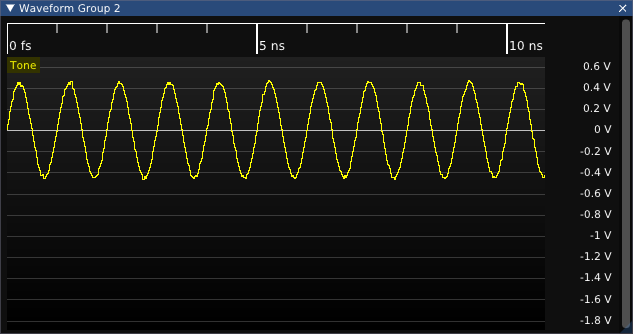
\includegraphics[width=13cm]{ng-images/y-divs.png}
\caption{Example waveform showing off-center grid and round-numbered grid lines}
\label{y-divs}
\end{figure}

Rather than optimizing for a touch screen (as is common for benchtop oscilloscopes), ngscopeclient's UI is
heavily mouse driven and context based. Space used by always-visible buttons, sliders, etc is kept to a minimum in
order to keep as much screen real estate as possible usable for waveform display. Additional controls are displayed in
menus or pop-up dialogs which can be closed, moved out of view, or docked as needed.

\section{Revision History}
\begin{itemize}
\item \today: [in progress] Initial draft
\end{itemize}

\chapter{Legal Notices}

\section{Introduction}

ngscopeclient, libscopehal, and the remainder of the project are all released under the 3-clause BSD license
(reproduced below). This is a permissive license, explicitly chosen to encourage integration with third-party open
source and commercial projects.

\section{License Agreement}

Copyright (c) 2012-2023 Andrew D. Zonenberg and contributors.
All rights reserved.

Redistribution and use in source and binary forms, with or without modification, are permitted provided that the
following conditions are met:
\begin{itemize}
\item Redistributions of source code must retain the above copyright notice, this list of conditions, and the
following disclaimer.
\item Redistributions in binary form must reproduce the above copyright notice, this list of conditions, and the
following disclaimer in the documentation and/or other materials provided with the distribution.
\item Neither the name of the author nor the names of any contributors may be used to endorse or promote products
derived from this software without specific prior written permission.
\end{itemize}

THIS SOFTWARE IS PROVIDED BY THE AUTHORS "AS IS" AND ANY EXPRESS OR IMPLIED WARRANTIES, INCLUDING, BUT NOT LIMITED
TO, THE IMPLIED WARRANTIES OF MERCHANTABILITY AND FITNESS FOR A PARTICULAR PURPOSE ARE DISCLAIMED. IN NO EVENT SHALL
THE AUTHORS BE HELD LIABLE FOR ANY DIRECT, INDIRECT, INCIDENTAL, SPECIAL, EXEMPLARY, OR CONSEQUENTIAL DAMAGES
(INCLUDING, BUT NOT LIMITED TO, PROCUREMENT OF SUBSTITUTE GOODS OR SERVICES; LOSS OF USE, DATA, OR PROFITS; OR
BUSINESS INTERRUPTION) HOWEVER CAUSED AND ON ANY THEORY OF LIABILITY, WHETHER IN CONTRACT, STRICT LIABILITY, OR TORT
(INCLUDING NEGLIGENCE OR OTHERWISE) ARISING IN ANY WAY OUT OF THE USE OF THIS SOFTWARE, EVEN IF ADVISED OF THE
POSSIBILITY OF SUCH DAMAGE.

\section{Trademarks}

This document frequently mentions the names of various test equipment vendors and products in order to discuss
ngscopeclient's compatibility with said products. The reader should assume that these are all trademarks of their
respective owners.

\section{Third Party Licenses}

TODO: go through full dependency list and update this
\begin{itemize}
\item Dear ImGui (static, MIT license)
\item FFTS (shared, BSD-3)
\item imgui-node-editor (static, MIT license)
\item liblxi (shared, BSD-3/EPICS)
\item vkFFT (static, MIT license)
\item yaml-cpp (shared, MIT license)
\end{itemize}

\subsection{avx\_mathfun.h (zlib license)}

AVX implementation of sin, cos, sincos, exp and log

Based on "sse\_mathfun.h", by Julien Pommier
http://gruntthepeon.free.fr/ssemath/

Copyright (C) 2012 Giovanni Garberoglio
Interdisciplinary Laboratory for Computational Science (LISC)
Fondazione Bruno Kessler and University of Trento
via Sommarive, 18
I-38123 Trento (Italy)

This software is provided 'as-is', without any express or implied
warranty.  In no event will the authors be held liable for any damages
arising from the use of this software.

Permission is granted to anyone to use this software for any purpose,
including commercial applications, and to alter it and redistribute it
freely, subject to the following restrictions:

\begin{enumerate}
\item The origin of this software must not be misrepresented; you must not
claim that you wrote the original software. If you use this software
in a product, an acknowledgment in the product documentation would be
appreciated but is not required.
\item Altered source versions must be plainly marked as such, and must not be
misrepresented as being the original software.
\item This notice may not be removed or altered from any source distribution.
\end{enumerate}

\chapter{Getting Started}

\section{Documentation Conventions}

Items to be selected from a menu are displayed in \menustyle{monospace font}.

Multilevel menu paths are separated by a / character. For example, \menustyle{Attenuation / 1x} means to open the
\menustyle{Attenuation} submenu and select the \menustyle{1x} item.

If there are multiple options for a menu or configuration option, they are displayed in square brackets and separated
by a | character. For example, \menustyle{Move waveform to / Waveform Group [1|2]} means to select either
\menustyle{Waveform Group 1} or \menustyle{Waveform Group 2} from the \menustyle{Move waveform to}
menu.

This project is under active development and is not anywhere near feature complete! As a result, this document is
likely to refer to active bug or feature request tickets on the GitHub issue trackers. Issues are referenced as
repository:ticket, for example \issue{scopehal-apps}{3}.

\section{Host System Requirements}

The majority of development is performed on Linux operating systems (primarily Debian and Arch) so this is the most well
tested platform, however Windows and Mac OS are also supported.

Any 64-bit Intel or AMD processor, or Apple Silicon Mac, should be able to run ngscopeclient. If AVX2 and/or AVX512F
support is present ngscopeclient will use special optimized versions of some signal processing functions, however
neither instruction set is required. Other (non Apple Silicon) ARM64 platforms may work if a compatible GPU is
available, but have not been tested. 32-bit platforms are not supported due to the significant RAM requirements.

A mouse with scroll wheel, or touchpad with scroll gesture support, is mandatory to enable full use of the UI. We may
explore alternative input methods for some UI elements in the future.

Any GPU with Vulkan support should be able to run ngscopeclient, however Vulkan 1.2 will deliver better performance.
The minimum supported GPUs are:
\begin{itemize}
\item AMD: GCN based (Radeon HD 7000 and newer, January 2012)
\item Apple: all Apple Silicon devices (M1 and newer)
\item Intel: Iris Plus 540 or HD Graphics 520 (Skylake, August 2015)
\item NVIDIA: Maxwell architecture (GeForce GTX 700 series and newer, February 2014)
\end{itemize}

The minimum RAM requirement to actually launch ngscopeclient is relatively small, however actual memory consumption is
heavily dependent on workload and can easily reach into the tens of gigabytes when doing complex analysis on many
channels with deep history.

Typical RAM consumption examples:
\begin{itemize}
\item Default configuration with demo scope (4 channels 100K points, 10 waveforms of history, no analysis): 250 MB
\item 4M point live streaming with 10 waveforms of history, eye pattern, 8B/10B decode, and jitter histogram: 650 MB
\item Single 512M point waveform, no analysis or history: 2.1 GB
\item 512M point P/N channel waveforms with CDR and eye pattern, no history: 8.3 GB
\end{itemize}

Large amounts of GPU RAM are required for working with deep waveforms, especially if you intend to perform
complex analysis on them. Analog waveforms are stored in 32-bit floating point format internally, so a single 256
megapoint waveform will consume 1GB of GPU memory. Intermediate results in multi-step filter pipelines require GPU
memory as well, even if not displayed.

\section{Instrument Support}

ngscopeclient uses the libscopehal library to communicate with instruments, so any libscopehal-compatible hardware
should work with ngscopeclient. See the \hyperref[sec:scope-drivers]{Oscilloscope Drivers} section for more details on
which hardware is supported and how to configure specific drivers.

\section{Compilation}

ngscopeclient can be compiled on Linux, macOS, and Windows, but the specific steps that have to be taken differ quite a
lot between these the three.

TODO: rewrite and simplify this section once we've removed all remaining vestiges of GTK dependencies

TODO: update URLs for most recent tested Vulkan SDK revision

\subsection{Linux}
\begin{enumerate}

\item Install dependencies.

On Debian/Ubuntu:

\begin{lstlisting}[language=sh, numbers=none]
sudo apt install build-essential cmake pkg-config libglm-dev \
	libgtkmm-3.0-dev libsigc++-2.0-dev libyaml-cpp-dev \
	liblxi-dev texlive texlive-fonts-extra texlive-extra-utils \
	libglew-dev catch2 libvulkan-dev glslang-dev libglfw3-dev
\end{lstlisting}

On Fedora:

\begin{lstlisting}[language=sh, numbers=none]
sudo dnf install gcc-g++ ccache make cmake pkg-config glm-devel \
	gtkmm3.0-devel libsigc++30-devel libyaml-devel yaml-cpp-devel \
	liblxi-devel libtirpc-devel texlive glew-devel \
	catch2-devel vulkan-loader-devel glslang-devel glfw-devel \
	glslc libshaderc-devel libshaderc-static \
	spirv-tools-devel
\end{lstlisting}

If you are using an older stable release (such as Debian Buster), you may need to install catch2 from source
(https://github.com/catchorg/Catch2). Alternatively, you may pass -DBUILD\_TESTING=OFF to CMake to disable unit testing.

\item Install FFTS library:

\begin{lstlisting}[language=sh, numbers=none]
cd ~
git clone https://github.com/anthonix/ffts.git
cd ffts
mkdir build
cd build
cmake .. -DENABLE_SHARED=ON -DCMAKE_INSTALL_PREFIX=/usr
make -j4
sudo make install
\end{lstlisting}

\item Install Vulkan SDK:

If you are using Debian or Ubuntu, you may also install the
\href{https://vulkan.lunarg.com/doc/sdk/1.3.261.1/linux/getting_started_ubuntu.html}{.deb packaged SDK release} instead
of following the instructions below.

On Fedora, the SDK is already installed above, and the following section should be skipped.

\begin{lstlisting}[language=sh, numbers=none]
cd ~
mkdir vulkan
cd vulkan
wget https://sdk.lunarg.com/sdk/download/1.3.250.1/linux/vulkansdk-linux-x86_64-1.3.250.1.tar.gz
tar xf vulkansdk-linux-x86_64-1.3.250.1.tar.gz
rm -f vulkansdk-linux-x86_64-1.3.250.1.tar.gz
export VULKAN_SDK=~/vulkan/1.3.250.1/x86_64
sudo cp -r $VULKAN_SDK/include/vulkan/ /usr/local/include/
sudo cp -P $VULKAN_SDK/lib/libvulkan.so* /usr/local/lib/
sudo cp $VULKAN_SDK/lib/libVkLayer_*.so /usr/local/lib/
sudo mkdir -p /usr/local/share/vulkan/explicit_layer.d
sudo cp $VULKAN_SDK/etc/vulkan/explicit_layer.d/VkLayer_*.json \
	/usr/local/share/vulkan/explicit_layer.d
sudo ldconfig
\end{lstlisting}

\item Build scopehal and scopehal-apps:

\begin{lstlisting}[language=sh, numbers=none]
# On Fedora, skip the following exports:
export VULKAN_SDK=~/vulkan/1.3.250.1/x86_64
export PATH=$VULKAN_SDK/bin:$PATH
export LD_LIBRARY_PATH=$VULKAN_SDK/lib${LD_LIBRARY_PATH:+:$LD_LIBRARY_PATH}
export VK_LAYER_PATH=$VULKAN_SDK/etc/vulkan/explicit_layer.d

cd ~
git clone --recursive https://github.com/ngscopeclient/scopehal-apps.git
cd scopehal-apps
mkdir build
cd build
cmake ../ -DCMAKE_BUILD_TYPE=Release -DCMAKE_INSTALL_PREFIX=/usr
make -j4
\end{lstlisting}

\item Install scopehal and scopehal-apps:

\begin{lstlisting}[language=sh, numbers=none]
cd ~/scopehal-apps/build
sudo make install
\end{lstlisting}

\end{enumerate}

\subsection{macOS}
\begin{enumerate}

\item Install dependencies.

With Homebrew (\href{https://brew.sh}{brew.sh}):

\begin{lstlisting}[language=sh, numbers=none]
brew install pkg-config gtk+3 gtkmm3 glfw cmake yaml-cpp glew catch2 libomp
\end{lstlisting}

\item Install Vulkan SDK:

Download and install the Vulkan SDK from \href{https://sdk.lunarg.com/sdk/download/1.3.231.1/mac/vulkansdk-macos-1.3.231.1.dmg}{sdk.lunarg.com/sdk/download/1.3.231.1/mac/vulkansdk-macos-1.3.231.1.dmg}.

\item Build scopehal and scopehal-apps:

\begin{lstlisting}[language=sh, numbers=none]
export VULKAN_SDK=~/VulkanSDK/1.3.231.1/macOS
export PATH=${PATH}:${VULKAN_SDK}/bin:/opt/homebrew/bin
cd ~
git clone --recursive https://github.com/ngscopeclient/scopehal-apps.git
cd scopehal-apps
mkdir build
cd build
cmake ../ -DCMAKE_BUILD_TYPE=Release -DCMAKE_INSTALL_PREFIX=/usr \
	-DCMAKE_PREFIX_PATH="/opt/homebrew;/opt/homebrew/opt/libomp"
make -j4
\end{lstlisting}

\item Install scopehal and scopehal-apps:

Installation on macOS is not yet complete.
The binaries can be found in the build directory, such as ngscopeclient in \$HOME/scopehal-apps/build/src/ngscopeclient.

\end{enumerate}

\subsection{Windows}

On Windows, we make use of the MSYS2 development environment, which gives us access to the MingGW-w64 toolchain.
Since this toolchain allows ngscopeclient to be compiled as a native Windows application, the project might be run
outside of MSYS2.

\subsubsection{Installing from the package manager}

\begin{lstlisting}[language=sh, numbers=none]
pacman -Sy
pacman -S mingw-w64-x86_64-scopehal-apps
\end{lstlisting}

See also \href{https://packages.msys2.org/group/mingw-w64-x86_64-eda}{\lstinline{mingw-w64-x86_64-eda}}.

\subsubsection{Building from source}

\begin{enumerate}

\item Download and install MSYS2. You can download it from \href{https://www.msys2.org/}{msys2.org} or \href{https://github.com/msys2/msys2-installer/releases}{github.com/msys2/msys2-installer/releases}\\
It is of utmost importance that \textbf{all} steps outlined on the website are followed precisely, even if they might
seem unnecessary.
This will avoid lots of hard to diagnose problems later on in the build.\\

All following steps are to be done in a MinGW64 shell (\textbf{not} in a MSYS, MINGW32, CLANG64, CLANG32 or UCRT64 shell,
which also get installed by the MSYS2 installer).

\item Install WiX Toolset v3.11 (required to build the Windows x64 MSI)
You shall download and install WiX Toolset v3.11 in \begin{verbatim}C:\Program Files (x86)\WiX Toolset v3.11\end{verbatim}
https://wixtoolset.org/docs/wix3/

\item Install git and the toolchain:

\begin{lstlisting}[language=sh, numbers=none]
pacman -S git wget mingw-w64-x86_64-cmake mingw-w64-x86_64-toolchain
\end{lstlisting}

\item Build glslang tags/sdk-1.3.224.1:

Launch MSYS2 or MINGW64 as Administrator only for this step (it is mandatory to do the install in default path C:\\VulkanSDK ...)
\begin{lstlisting}[language=sh, numbers=none]
# Windows mingw64 glslang build (as it is not fully integrated in
# VulkanSDK-1.3.224.1 for Windows and built with Visual Studio 2017)
cd ~
git clone https://github.com/KhronosGroup/glslang.git
cd glslang
git checkout tags/sdk-1.3.224.1
git clone https://github.com/google/googletest.git External/googletest
cd External/googletest
git checkout 0c400f67fcf305869c5fb113dd296eca266c9725
cd ../..
./update_glslang_sources.py

SOURCE_DIR=~/glslang
BUILD_DIR=$SOURCE_DIR/build
mkdir -p $BUILD_DIR
cd $BUILD_DIR
cmake -DCMAKE_BUILD_TYPE=Release -G"MinGW Makefiles" $SOURCE_DIR \
	-DCMAKE_INSTALL_PREFIX="$(pwd)/install"
cmake --build . --config Release --target install
\end{lstlisting}

\item Install Vulkan SDK:

Launch MSYS2 or MINGW64 as Administrator only for this step (it is mandatory to do the install in default path C:\\VulkanSDK ...)
\begin{lstlisting}[language=sh, numbers=none]
cd ~
wget https://sdk.lunarg.com/sdk/download/1.3.224.1/windows/VulkanSDK-1.3.224.1-Installer.exe
./VulkanSDK-1.3.224.1-Installer.exe --accept-licenses --default-answer \
	--confirm-command install
rm -f VulkanSDK-1.3.224.1-Installer.exe
\end{lstlisting}

\item Check out the code

\begin{lstlisting}[language=sh, numbers=none]
cd ~
git clone --recursive https://github.com/ngscopeclient/scopehal-apps
\end{lstlisting}

\item Execute makepkg-mingw in subdir MSYS2:

\begin{lstlisting}[language=sh, numbers=none]
cd ~/scopehal-apps/msys2
export VK_SDK_PATH=/c/VulkanSDK/1.3.224.1
export PATH=$VK_SDK_PATH/Bin:$PATH
export VULKAN_SDK=$VK_SDK_PATH
export GLSLANG_BUILD_PATH=~/glslang/build/install

MINGW_ARCH=mingw64 makepkg-mingw --noconfirm --noprogressbar -sCLf
\end{lstlisting}

The unit tests will not be run as part of this build - if you would like to run them, you will need to provide catch2
(https://github.com/catchorg/Catch2), and remove the -DBUILD\_TESTING=OFF flag from the PKGBUILD recipe in subdir
msys2.

\item Installing, copying binaries and running ngscopeclient.

Since ngscopeclient is built using the MinGW toolchain, it depends on a rather large number of dynamic libraries.
The recommended procedure is to install the package generated by makepkg-mingw on a MinGW64 shell:

\begin{lstlisting}[language=sh, numbers=none]
cd ~
cd msys2
pacman -U *.zst
\end{lstlisting}

This is equivalent to the package installed through \lstinline{pacman -S}, but it's built from the checked out commit,
instead of the pinned version available from MSYS2 repositories.

The \lstinline{*.zst} package includes metadata about the dependencies.
Therefore, when installed through \lstinline{pacman}, those will be installed automatically.
However, some users might want to use ngscopeclient outside of MSYS2.
In those cases, it needs to be installed first, and then a tarball/zipfile can be created by collecting all the dependencies.
This last approach is not officially supported yet.

\end{enumerate}

\section{Running ngscopeclient}

When running ngscopeclient with no arguments, an empty session (Fig. \ref{empty-window}) is created. To perform useful
work, you can:
\begin{itemize}
\item Open a saved session and reconnect to the instruments (\menustyle{File | Open Online})
\item Open a saved session without reconnecting to the instruments (\menustyle{File | Open Offline})
\item Open a recently used session (\menustyle{File | Recent Files})
\item Import waveforms from a third party file format(\menustyle{Add | Import})
\item Connect to an instrument (\menustyle{Add | Oscilloscope}, \menustyle{Add | Multimeter}, etc.)
\item Generate a synthetic waveform (\menustyle{Add | Generate})
\end{itemize}

\begin{figure}[h]
\centering
	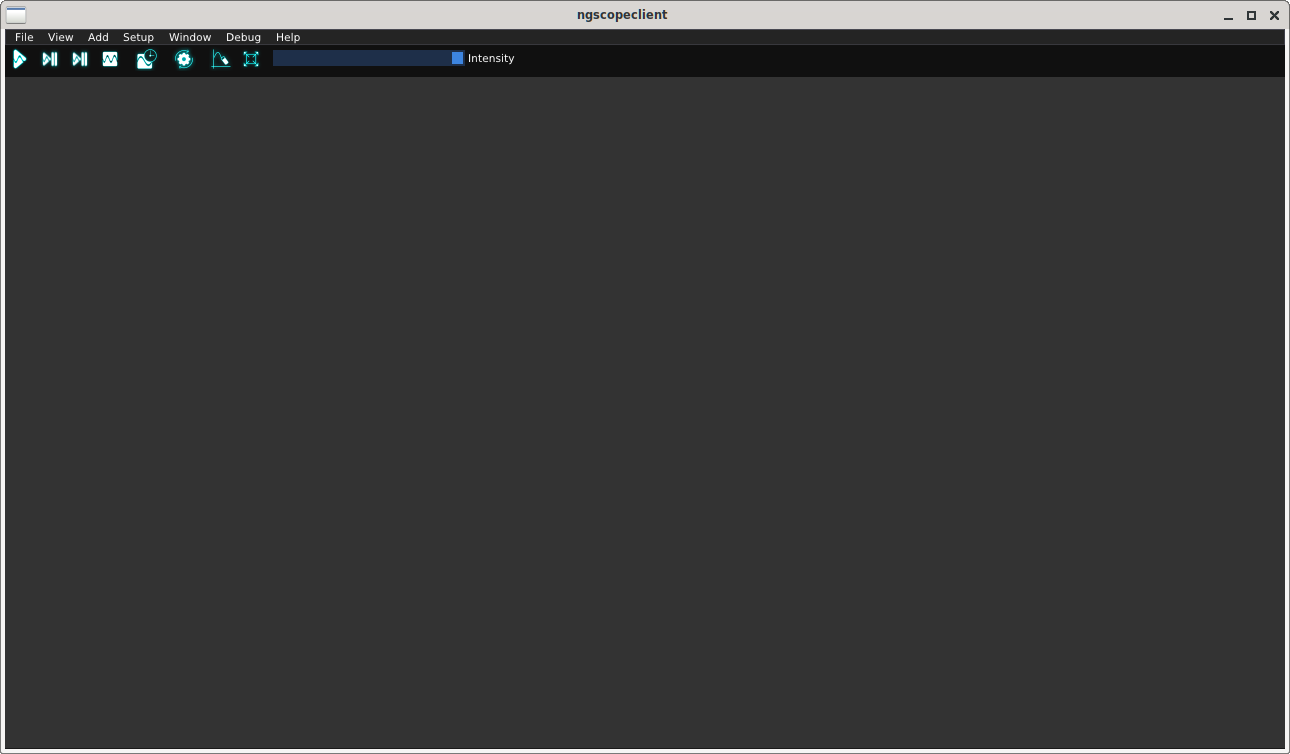
\includegraphics[width=12cm]{ng-images/empty-window.png}
\caption{Empty ngscopeclient session}
\label{empty-window}
\end{figure}

% TODO: add this section once these are implemented
\begin{comment}

\subsection{Configuration arguments}

Most of these arguments are intended for developers, but they can help troubleshoot unusual bugs.

\begin{itemize}

\item \texttt{--noavx2}\\
Do not use AVX2 vector optimizations even if the CPU supports it.

\item \texttt{--noavx512f}\\
Do not use AVX512F vector optimizations even if the CPU supports it.

\item \texttt{--noglint64}\\
Do not use \texttt{GL\_ARB\_gpu\_shader\_int64} even if the GPU supports it.

\item \texttt{--nogpufilter}\\
Do not use Vulkan (GPU accelerated) implementations of filter blocks, revert to software fallback.

\end{itemize}

\end{comment}

\subsection{Console verbosity arguments}

ngscopeclient takes standard liblogtools arguments for controlling console debug verbosity.

If no verbosity level is specified, the default is ``notice" (3). (We suggest using \texttt{--debug} for routine use
until the v1.0 release to aid in troubleshooting.)

\begin{itemize}

\item \texttt{--debug}\\
Sets the verbosity level to ``debug" (5).

\item \texttt{-l [file]}, \texttt{--logfile [file]}\\
Writes a copy of all log messages to \texttt{file}. This is preferred over simply redirecting output with pipes, as
console escape sequences are stripped from the file log output.

\item \texttt{-L [file]}, \texttt{--logfile-lines [file]}\\
Same as \texttt{--logfile} except line buffering is turned on.

\item \texttt{-q}, \texttt{--quiet}\\
Reduces the verbosity level by one. Can be specified more than once to lower verbosity by several steps.

\item \texttt{--trace [class]}, \texttt{--trace [class::function]} \\
Enables extra debug output from the class \texttt{class} or the function \texttt{class::function}. Has no effect unless
\texttt{--debug} is also specified.

\item \texttt{--stdout-only}\\
Sends all logging output to stdout. By default, error (level 1) and warning (level 2) messages go to stderr.

\item \texttt{--verbose}\\
Sets the verbosity level to ``verbose" (4).

\end{itemize}

% TODO: add this section once these are implemented
\begin{comment}
\subsection{File arguments}
\label{import}

The file extension is used to determine the format. File extensions are case sensitive and must be lowercase to be
correctly interpreted.

\begin{itemize}
\item \texttt{[file.scopesession]}
Loads a saved session.

\item \texttt{[file.bin]} \\
Imports waveform data from the binary format used by Agilent, Keysight, and Rigol oscilloscopes.

\item \texttt{[file.complex]} \\
Imports complex I/Q data from a file. The file must contain interleaved (I, Q) pairs in either 8-bit signed/unsigned
integer, 16-bit signed integer, 32-bit normalized floating point, or 64-bit normalized floating point format.

The default format is 8 bit signed integer and may be changed from the filter graph editor or channel properties dialog
once the file is loaded. There is currently no way to specify other formats on the command line.

\item \texttt{[file.csv]} \\
Imports sample data from a CSV (comma-separated-value) file. More than one CSV file can be loaded at once (displayed as
separate points in history) by specifying multiple file names as long as they have identical column schemas.

Lines starting with a '\#' character are treated as comments and generally ignored by the parser. (If the comment format
matches that used by Digilent's WaveForms utility, timestamps and other metadata are extracted from the comments.)

If the first row of the CSV contains non-numeric characters, it is treated as a header row. Header content in the
timestamp column is ignored; headers in other columns are used as channel names in the imported waveform.

The first column of the CSV must contain sample timestamps, in seconds. Scientific notation is supported. Timestamps
must be monotonic (each row must have a timestamp strictly greater than that of the previous row).

ngscopeclient uses a heuristic to detect uniformly sampled waveforms, which enabled certain optimizations for display
and signal processing. If the standard deviation of intervals between samples is less than 1\% of the average sample
interval, the waveform is assumed to be uniformly sampled and timestamps are rounded to the nearest multiple of the
average interval. If the deviation is greater, the waveform is assumed to be sparsely sampled and timestamps are not
modified.

\item \texttt{[file.trc]} \\
Imports waveform data from a Teledyne LeCroy .trc binary waveform file.

\item \texttt{[file.vcd]} \\
Imports digital waveform data from a VCD (value change dump) file, typically created by a logic analyzer or HDL
simulator.

\item \texttt{[file.wav]} \\
Imports sample data from a WAV file.

\item \texttt{[file.wfm]} \\
Imports sample data from a Tektronix .wfm file. This import filter is still experimental and may not support all
features of the .wfm file format yet. If you have trouble importing some .wfm files please file a ticket on GitHub.

%%%%%%%%%%%%%%%%%%%%%%%%%%%%%%%%%%%%%%%%

\item \texttt{--nodata}\\
When loading a .scopesession file, load settings only and not saved waveform data.

\item \texttt{--reconnect}\\
When loading a .scopesession file, reconnect to the instrument and resume remote control. Current instrument settings
are overwritten with the configuration from the saved session.

\item \texttt{--retrigger}\\
When loading a .scopesession file, arm the trigger immediately. has no effect unless \texttt{--reconnect} is also
specified.

\end{itemize}

\subsection{Instrument arguments}

Example:
\begin{lstlisting}[language=sh, numbers=none]
./ngscopeclient --debug \
	mylecroy:lecroy:vicp:myscope.example.com:1234 \
	myrigol:rigol:lan:rigol.example.com
\end{lstlisting}

\begin{itemize}
\item \texttt{[connection string]} \\
Connects to the specified instrument. By default, all channels are enabled and displayed.

\end{itemize}

Each instrument is described by a ``connection string" containing four colon-separated fields.

\begin{itemize}
\item Nickname. This can be any text string not containing spaces or colons. If you have only one instrument it's
largely ignored, but when multiple instruments are present channel names in the UI are prefixed with the nickname to
avoid ambiguity.
\item Driver name. This is a string identifying the command protocol the scope uses. Note that not all
scopes from the same vendor will use the same command set or driver!
\item Transport. This is is a string describing how the driver connects to the scope (e.g. RS232 or Ethernet)
\item Arguments for the driver identifying the device to connect to, separated by colons. This varies by driver but is
typically a hostname:port combination, TTY device path, or similar.
\end{itemize}

\end{comment}

\chapter{Main Window}

The only fixed UI elements in ngscopeclient are the main menu and toolbar at the top of the window. All remaining space
may be filled with waveform plots, properties dialogs, protocol analyzers, and other dockable windows as required for a
given experimental setup. This flexibility allows almost the entire screen to be dedicated to waveform views, or more
space allocated to controls and protocol decodes.

\section{Menu}

%%%%%%%%%%%%%%%%%%%%%%%%%%%%%%%%%%%%%%%%%%%%%%%%%%%%%%%%%%%%%%%%%%%%%%%%%%%%%%%%%%%%%%%%%%%%%%%%%%%%%%%%%%%%%%%%%%%%%%%%
\subsection{File}

This menu contains commands for saving and loading session files.

\begin{itemize}

\item \menustyle{Open Online...}\\
Loads a session file and reconnects to the instrument(s) to continue existing work. Settings from the saved
session will be applied and overwrite the current channel and timebase configuration of the instrument, if different.

\item \menustyle{Open Offline...}\\
Loads a session file in offline mode, allowing you to work with saved waveform data without connecting to the
instrument(s) the data was captured from.

\item \menustyle{Recent Files}\\
Displays a list of recently accessed session files and allows them to be opened online or offline.

\item \menustyle{Save}\\
Saves UI configuration and waveform data (including history) to a session file for future use.

A session consists of a YAML file called \emph{filename}.scopesession containing instrument and UI configuration, as
well as a directory called \emph{filename}\_data which contains waveform metadata and sample values for all enabled
instrument channels, including history.

Note that both the .scopesession and the \_data directory must be copied if moving the session to a new location in
order to preserve waveform data. If you only wish to restore the filter graph and UI configuration without waveform
content, the \_data directory is not required.

\item \menustyle{Save As...}\\
Saves the session to a new file, rather than the current one.

\item \menustyle{Close}\\
Close the current session without exiting ngscopeclient.

\item \menustyle{Quit}\\
Exits the application

\end{itemize}

%%%%%%%%%%%%%%%%%%%%%%%%%%%%%%%%%%%%%%%%%%%%%%%%%%%%%%%%%%%%%%%%%%%%%%%%%%%%%%%%%%%%%%%%%%%%%%%%%%%%%%%%%%%%%%%%%%%%%%%%
\subsection{View}

\begin{itemize}

\item \menustyle{Fullscreen}\\
Toggles full-screen mode

\item \menustyle{Persistence Setup}\\
Opens the Persistence Setup dialog, allowing you to control the decay coefficient for persistence maps.

\end{itemize}

%%%%%%%%%%%%%%%%%%%%%%%%%%%%%%%%%%%%%%%%%%%%%%%%%%%%%%%%%%%%%%%%%%%%%%%%%%%%%%%%%%%%%%%%%%%%%%%%%%%%%%%%%%%%%%%%%%%%%%%%
\subsection{Add}

This menu allows new waveforms views or instrument connections to be created.

\begin{itemize}

\item \menustyle{Load}\\
Connect to a new, or recently used, electronic load

\item \menustyle{Generator}\\
Connect to a new, or recently used, function generator

\item \menustyle{Multimeter}\\
Connect to a new, or recently used, multimeter

\item \menustyle{Oscilloscope}\\
Connect to a new, or recently used, oscilloscope

\item \menustyle{Power Supply}\\
Connect to a new, or recently used, power supply

\item \menustyle{RF Generator}\\
Connect to a new, or recently used, RF signal generator

\item \menustyle{Channels}\\
Displays a list of filters and instrument channels which can be opened in a new waveform view

\item \menustyle{Generate}\\
Allows synthetic waveforms to be generated for testing, simulation, and channel design applications

\item \menustyle{Import}\\
Allows waveforms to be loaded from external data files in various interchange formats

\end{itemize}

%%%%%%%%%%%%%%%%%%%%%%%%%%%%%%%%%%%%%%%%%%%%%%%%%%%%%%%%%%%%%%%%%%%%%%%%%%%%%%%%%%%%%%%%%%%%%%%%%%%%%%%%%%%%%%%%%%%%%%%%
\subsection{Setup}

\begin{itemize}

%\item \menustyle{Instrument Sync}\\
%Synchronizes two or more instruments under a single ngscopeclient instance. TODO: more complete documentation

\item \menustyle{Timebase...}\\
Opens the Timebase Properties dialog, allowing sample rate and memory depth of each connected oscilloscope to be
adjusted

\item \menustyle{Trigger...}\\
Configures trigger settings

%\item \menustyle{Halt Conditions}\\
%Makes ngscopeclient pause when a waveform meeting certain conditions is acquired

\item \menustyle{Preferences...}\\
Opens the preferences dialog

\end{itemize}

\begin{comment}

\begin{tabularx}{16cm}{llX}
\thickhline
\textbf{Name} & \textbf{Colors} & \textbf{Notes} \\
\thickhline
CRT & \includegraphics[width=5cm]{images/eye-gradient-crt.png} & Similar to a major vendor's color scheme.\\
Grayscale & \includegraphics[width=5cm]{images/eye-gradient-grayscale.png} & Common monochrome palette.\\
Ironbow & \includegraphics[width=5cm]{images/eye-gradient-ironbow.png} & Common "hot metal" palette. \\
KRain & \includegraphics[width=5cm]{images/eye-gradient-krain.png} & Similar to a major vendor's color scheme.\\
Rainbow & \includegraphics[width=5cm]{images/eye-gradient-rainbow.png} & Common HSV rainbow palette. \\
Reverse Rainbow & \includegraphics[width=5cm]{images/eye-gradient-reverse-rainbow.png} & Common HSV rainbow palette. \\
Viridis & \includegraphics[width=5cm]{images/eye-gradient-viridis.png} & Perceptually uniform palette from matplotlib. \\
\thickhline
\end{tabularx}

\end{comment}

%%%%%%%%%%%%%%%%%%%%%%%%%%%%%%%%%%%%%%%%%%%%%%%%%%%%%%%%%%%%%%%%%%%%%%%%%%%%%%%%%%%%%%%%%%%%%%%%%%%%%%%%%%%%%%%%%%%%%%%%
\subsection{Window}

This menu provides access to various utility windows.

\begin{itemize}

\item \menustyle{Analyzer}\\
Opens protocol analyzer dialogs for active protocol decodes

\item \menustyle{Generator}\\
Opens the properties dialog for a currently connected function generator

\item \menustyle{Multimeter}\\
Opens the properties dialog for a currently connected multimeter

\item \menustyle{SCPI Console}\\
Opens a console window allowing you to send raw SCPI commands to a currently connected instrument.

This is a low level debug tool primarily intended for use by driver developers. The console is interlocked with
background threads polling the instrument, so that replies to commands typed in the console will not be mixed with
replies which the instrument driver is expecting to its own commands. However, commands sent in the console will bypass
any caching in the driver and can easily lead to the driver and instrument firmware states becoming mutually
inconsistent.

\item \menustyle{Log Viewer}\\
Opens a console window allowing you to see debug log messages generated by the application. This is the same log stream
which is normally written to stdout, but this dialog allows it to be accessed even when the application is not launched
from a shell session.

\item \menustyle{Measurements}\\
Opens the Measurements window, displaying scalar-valued measurements coming from instrument channels or filter blocks.

\item \menustyle{Performance Metrics}\\

Opens the Performance Metrics window, which provides access to debug information which can be helpful when debugging
slow application performance, optimizing the code, or benchmarking instruments.

Three categories of information are displayed:

\begin{itemize}
\item Rendering: render loop framerate, monitor refresh rate, total time spent last frame in the rasterization and tone
mapping shaders, and the number of vertices and indices drawn as Vulkan geometry. Note that waveforms are drawn by a
compute shader and do not contribute towads the vertex/index totals, other than a single textured rectangle used for
displaying the shader output.
\item Filter graph: number of filter blocks in the current graph, and run time for the most recent evaluation of the
filter graph.
\item Acquisition: streaming data rate, in waveforms per second.
\end{itemize}

\item \menustyle{History}\\

Opens the History dialog, which allows access to a rolling buffer of recently acquired waveforms.

\item \menustyle{Filter Graph}\\
Opens the filter graph editor (see Chapter \ref{grapheditor})

\end{itemize}

%%%%%%%%%%%%%%%%%%%%%%%%%%%%%%%%%%%%%%%%%%%%%%%%%%%%%%%%%%%%%%%%%%%%%%%%%%%%%%%%%%%%%%%%%%%%%%%%%%%%%%%%%%%%%%%%%%%%%%%%

\subsection{Debug}

Provides access to GUI toolkit test dialogs and other features intended only for developers.

%%%%%%%%%%%%%%%%%%%%%%%%%%%%%%%%%%%%%%%%%%%%%%%%%%%%%%%%%%%%%%%%%%%%%%%%%%%%%%%%%%%%%%%%%%%%%%%%%%%%%%%%%%%%%%%%%%%%%%%%

\subsection{Help}

Nothing here yet, we should add at least an About dialog at some point...

%\textbf{About}: Displays program version and copyright information

\begin{comment}
%%%%%%%%%%%%%%%%%%%%%%%%%%%%%%%%%%%%%%%%%%%%%%%%%%%%%%%%%%%%%%%%%%%%%%%%%%%%%%%%%%%%%%%%%%%%%%%%%%%%%%%%%%%%%%%%%%%%%%%%
\section{Toolbar}

The toolbar contains buttons and controls for the most frequently used actions.

\begin{figure}[h]
\centering
\includegraphics[width=16cm]{images/toolbar.png}
\caption{ngscopeclient toolbar}
\label{toolbar}
\end{figure}

\subsection{Capture buttons}

The capture button group (Fig. \ref{capturebuttons}) contains three buttons. From left to right these are ``arm
normal trigger", ``arm one-shot trigger" and ``stop trigger".

Note that the ``normal" trigger mode still uses one-shot capture internally so that all waveform data can be downloaded
before the next trigger event.

\begin{figure}[h]
\centering
\includegraphics[height=1cm]{images/capture-icons.png}
\caption{Capture control buttons}
\label{capturebuttons}
\end{figure}

\subsection{History}

The history button (Fig. \ref{historybutton}) toggles display of the \hyperref[sec:history]{waveform history view}.

\begin{figure}[h]
\centering
\includegraphics[height=1cm]{images/history-button.png}
\caption{History button}
\label{historybutton}
\end{figure}

\subsection{Refresh Settings}

In order to improve performance, ngscopeclient caches many instrument settings locally rather than constantly querying
the instrument for the current timebase, trigger configuration, etc. If settings are changed via the instrument front
panel while ngscopeclient is running, ngscopeclient may not be aware of these changes.

The Refresh Settings button (Fig. \ref{refreshbutton}) clears all cached instrument configuration and updates
ngscopeclient with the current instrument settings. For most ``headless" instruments, such as Pico Technology devices,
this button has no effect.

\begin{figure}[h]
\centering
\includegraphics[height=1cm]{images/refresh-button.png}
\caption{Refresh Settings button}
\label{refreshbutton}
\end{figure}

\subsection{Clear Sweeps}

The Clear Sweeps button (Fig. \ref{clearbutton}) clears all persistence waveforms, accumulated eye pattern / waterfall
data, and statistics. Waveforms saved in history are not deleted.

\begin{figure}[h]
\centering
\includegraphics[height=1cm]{images/clear-button.png}
\caption{Clear Sweeps button}
\label{clearbutton}
\end{figure}

\subsection{Fullscreen}

The Fullscreen button (Fig. \ref{fullscreenbutton}) switches ngscopeclient between normal and full-screen mode.

\begin{figure}[h]
\centering
\includegraphics[height=1cm]{images/fullscreen-button.png}
\caption{Fullscreen button}
\label{fullscreenbutton}
\end{figure}

\subsection{Opacity slider}

The opacity slider (Fig. \ref{opacityslider}) controls the alpha/opacity used to display intensity-graded waveforms.
Higher opacity values lead to better display of sparse waveforms (compare the crisp lines of Fig. \ref{sparse-waveform}
to the barely visible trace in Fig. \ref{dim-waveform}) but can lead to a washed-out appearance if too many sample
points are shoved into a small area.

\begin{figure}[H]
\centering
\includegraphics[height=1cm]{images/opacity-slider.png}
\caption{Trace opacity slider}
\label{opacityslider}
\end{figure}

\begin{figure}[H]
\centering
\includegraphics[width=10cm]{images/sparse-waveform.png}
\caption{Sparse waveform at a high zoom level}
\label{sparse-waveform}
\end{figure}

\begin{figure}[H]
\centering
\includegraphics[width=10cm]{images/dim-waveform.png}
\caption{Dim waveform showing difficulty of seeing waveform at low opacity}
\label{dim-waveform}
\end{figure}

For example, the DVI waveform in Fig. \ref{washedout-waveform} looks like a solid white blob with a vaguely visible
outline. No fine detail can be observed other than the increased over/undershoot and random-looking edges on the
scanlines, compared to the flat appearance of the blanking period between scanlines and at the end of the frame.

When the opacity is reduced in this example, many more nuances of the signal become apparent. The high/low voltage
levels of the signal compared to the transitions between them are obvious, and the H/V sync pulses within the blanking
period show up as a slightly darker region.

\begin{figure}[H]
\centering
\includegraphics[width=10cm]{images/washedout-waveform.png}
\caption{Intensity-graded waveform showing washed-out appearance at high opacity}
\label{washedout-waveform}
\end{figure}

\begin{figure}[H]
\centering
\includegraphics[width=10cm]{images/graded-waveform.png}
\caption{Intensity-graded waveform at lower opacity level}
\label{graded-waveform}
\end{figure}

As of this writing, the opacity setting is global for the entire application. Should this be changed to per waveform
group? If so, how should the group be selected and should there still be an option to make changes globally?
\end{comment}

\chapter{Dialogs}
\label{sec:dialogs}

%%%%%%%%%%%%%%%%%%%%%%%%%%%%%%%%%%%%%%%%%%%%%%%%%%%%%%%%%%%%%%%%%%%%%%%%%%%%%%%%%%%%%%%%%%%%%%%%%%%%%%%%%%%%%%%%%%%%%%%%

\section{Lab Notes}
\label{dlg:labnotes}

The Lab Notes dialog allows you to take notes on your experimental setup. It contains two tabs: ``setup notes"
and "general notes".

The contents of the Setup Notes tab are displayed on the \hyperref[dlg:speedbump]{Speed Bump} dialog when loading a
session file. The General Notes are only displayed within the Lab Notes dialog and are intended purely as a place for
recording interesting observations made during the experiment.

Minimal Markdown syntax (headings and bullets) is currently supported.\footnote{Images and links are supported by the
Markdown renderer library but the integration to properly use them is not yet finished; tables are not supported but
this will likely be added in the future.}

Lab notes are saved as Markdown files in the data directory for the session and can be opened in any
text editor or Markdown viewer. Note that they are overwritten each time the session is saved, so you should not modify
them using an external tool while the session is open in ngscopeclient or your changes may be lost.

\begin{figure}[H]
\centering
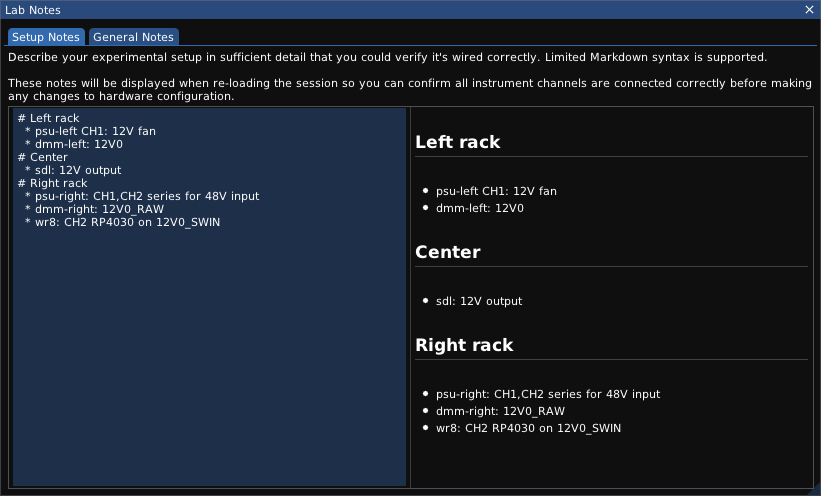
\includegraphics[width=12cm]{ng-images/dialog-labnotes.png}
\caption{Lab notes dialog}
\label{fig:labnotes}
\end{figure}


%%%%%%%%%%%%%%%%%%%%%%%%%%%%%%%%%%%%%%%%%%%%%%%%%%%%%%%%%%%%%%%%%%%%%%%%%%%%%%%%%%%%%%%%%%%%%%%%%%%%%%%%%%%%%%%%%%%%%%%%

\section{Preferences}
\label{dlg:preferences}

The Preferences dialog allows you to configure various application settings which are not specific to a particular
experimental setup. It can be found under the \menustyle{Setup | Preferences} menu.

\begin{figure}[H]
\centering
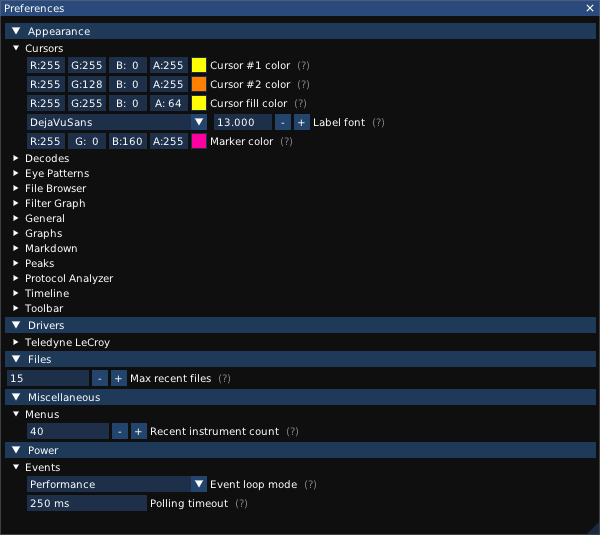
\includegraphics[width=7cm]{ng-images/dialog-preferences.png}
\caption{Preferences dialog}
\label{prefs}
\end{figure}

\subsection{Appearance}

This section allows you to configure fonts, colors, and other display settings for the application.

% TODO: document all of these preferences once the list has stabilized a bit

\subsection{Drivers}

This section allows you to configure default configurations for various instrument drivers.

\subsubsection{Teledyne LeCroy}

\begin{itemize}
\item \emph{Force 16 bit mode} (default on): Always use 16-bit format for downloading data from the instrument, even if
it only has an 8-bit ADC. This doubles the amount of network bandwidth required and may reduce waveforms-per-second
performance, but provides smoother waveforms since the instrument performs DSP flatness correction leading to >256
possible output values in a given waveform.
\end{itemize}

\subsection{Files}

\begin{itemize}
\item \emph{Max recent files}: Specify the number of files to display under the \menustyle{File | Recent Files} menu.
\end{itemize}

\subsection{Miscellaneous}

\subsubsection{Menus}

\begin{itemize}
\item \emph{Recent instrument count}: Specify the number of recently used instruments to remember
\end{itemize}

\subsection{Power}

\subsubsection{Events}

This section provides settings allowing power vs performance tradeoffs. The default settings are appropriate for a
desktop or laptop running on AC power; if running on a laptop with battery power you may wish to tune these to extend
battery lifespan.

\begin{itemize}
\item \emph{Event loop mode}: Controls the operating mode for the main application event loop.
\begin{itemize}
\item In Performance mode, run at the screen refresh rate. This allows for the highest possible waveform processing rate
and the smoothest interactivity, but may waste energy if you are spending a lot of time looking at the screen without
actively acquiring or processing waveforms.
\item In Power mode, run at a greatly reduced frequency (default 4 Hz but configurable by the Polling Timeout setting)
unless a redraw is triggered by mouse movement or keyboard input. This will limit the rate of waveform acquisition and
lead to a slightly jerkier user interface, but saves power.
\end{itemize}
\item \emph{Polling timeout}: If the event loop is in Power mode, specifies the timeout before the event loop will run
if there is no user input.
\end{itemize}

%%%%%%%%%%%%%%%%%%%%%%%%%%%%%%%%%%%%%%%%%%%%%%%%%%%%%%%%%%%%%%%%%%%%%%%%%%%%%%%%%%%%%%%%%%%%%%%%%%%%%%%%%%%%%%%%%%%%%%%%

\section{Speed Bump}
\label{dlg:speedbump}

The Speed Bump dialog is displayed when loading a session file, prior to committing changes to the instrument, if:

\begin{itemize}
\item The session file contains any user-created notes on the lab setup
\item Any of the instrument settings in the session file do not match the current configuration of the corresponding
instrument, and the direction of the change has potential to cause damage to the instrument or DUT (increasing output
voltage, removing input attenuation, etc).
\end{itemize}

This is intended as a safeguard to prevent damaging hardware by accidentally loading the wrong session file. It also
provides an opportunity to confirm that you have re-created the original experimental setup exactly if you are
switching a lab bench between multiple projects and using saved sessions to restore instrument state.

Pressing the Abort button cancels loading of the session without applying any of the potentially dangerous changes.
The instruments may be partially reconfigured in this state, as some changes (such as sample rate or memory depth
configuration) are always safe to make and thus may execute prior to the warning being displayed.

Pressing the Proceed button allows ngscopeclient to proceed with loading the session and reconfiguring hardware. You
must check the ``I have reviewed the instrument configuration" box in order to enable the Proceed button.

\begin{figure}[H]
\centering
\bigimage{ng-images/dialog-speedbump.png}
\caption{Speed Bump dialog}
\label{speedbump}
\end{figure}

%%%%%%%%%%%%%%%%%%%%%%%%%%%%%%%%%%%%%%%%%%%%%%%%%%%%%%%%%%%%%%%%%%%%%%%%%%%%%%%%%%%%%%%%%%%%%%%%%%%%%%%%%%%%%%%%%%%%%%%%

\section{Timebase}
\label{dlg:timebase}

The Timebase dialog allows you to configure sample rate and record length for oscilloscopes. It also provides control
over functionally similar ``what to look at" settings for other instruments, such as center frequency and span for
spectrum analyzers or sweep range and point count for vector network analyzers.

It can be found under the \menustyle{Setup | Timebase} menu.

\begin{figure}[H]
\centering
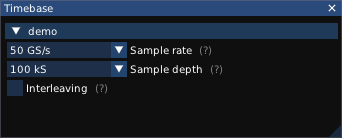
\includegraphics[width=7cm]{ng-images/dialog-timebase.png}
\caption{Timebase dialog}
\label{timebase}
\end{figure}

\chapter{Waveform Groups}

A waveform group is a collection of one or more waveform views stacked vertically under a common timeline. All waveform
views within a group are equally sized and share the same timeline and vertical cursor(s), but may have independent
vertical range and offset settings.

When a new oscilloscope is added to an empty ngscopeclient session, all enabled channels on the attached instrument(s)
are displayed in a single waveform group (Figure \ref{single-group}). If no channels are enabled at connection time,
the first channel will be enabled and displayed.

\begin{figure}[h]
\centering
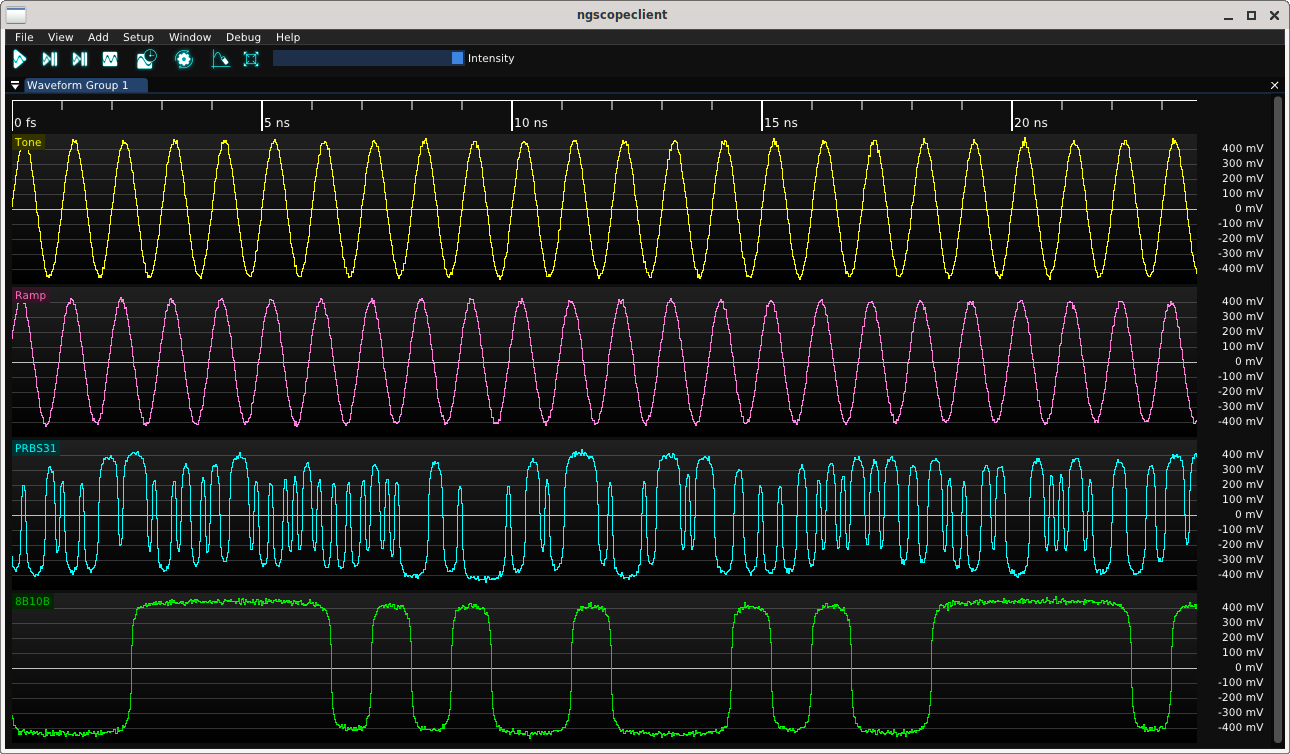
\includegraphics[width=13cm]{ng-images/overview.png}
\caption{Top level ngscopeclient window with a single waveform group}
\label{single-group}
\end{figure}

As you add protocol decodes or look at different parts of a waveform, it may be helpful to create additional waveform
groups. Typical reasons for creating additional groups include:

\begin{itemize}
\item Zooming into one set of signals to see detail on short time scales while maintaining a high level overview of
others
\item Viewing signals with incompatible horizontal units. For example, a FFT has horizontal units of frequency while an
analog waveform has horizontal units of time. Eye patterns also have horizontal units of time, but are always displayed
as two UIs wide and cannot be zoomed.
\end{itemize}

\section{Managing Groups}

New waveform groups are automatically created when adding a channel which is not compatible with any existing group.
For example, if your session has a single group containing time-domain waveforms, adding a FFT filter block will result
in a new waveform group being created to contain the FFT. Additional frequency-domain waveforms will then be added to
this group by default.

A new group may also be created at any time by clicking on a channel name and dragging it to the top, bottom, left, or
right edge of an existing group. An overlay (Fig. \ref{split-overlays}) will be displayed showing the resulting split.
For example, dropping the channel on the right side of the window produces the layout shown in Fig. \ref{split-right}.

\begin{figure}[h]
\centering
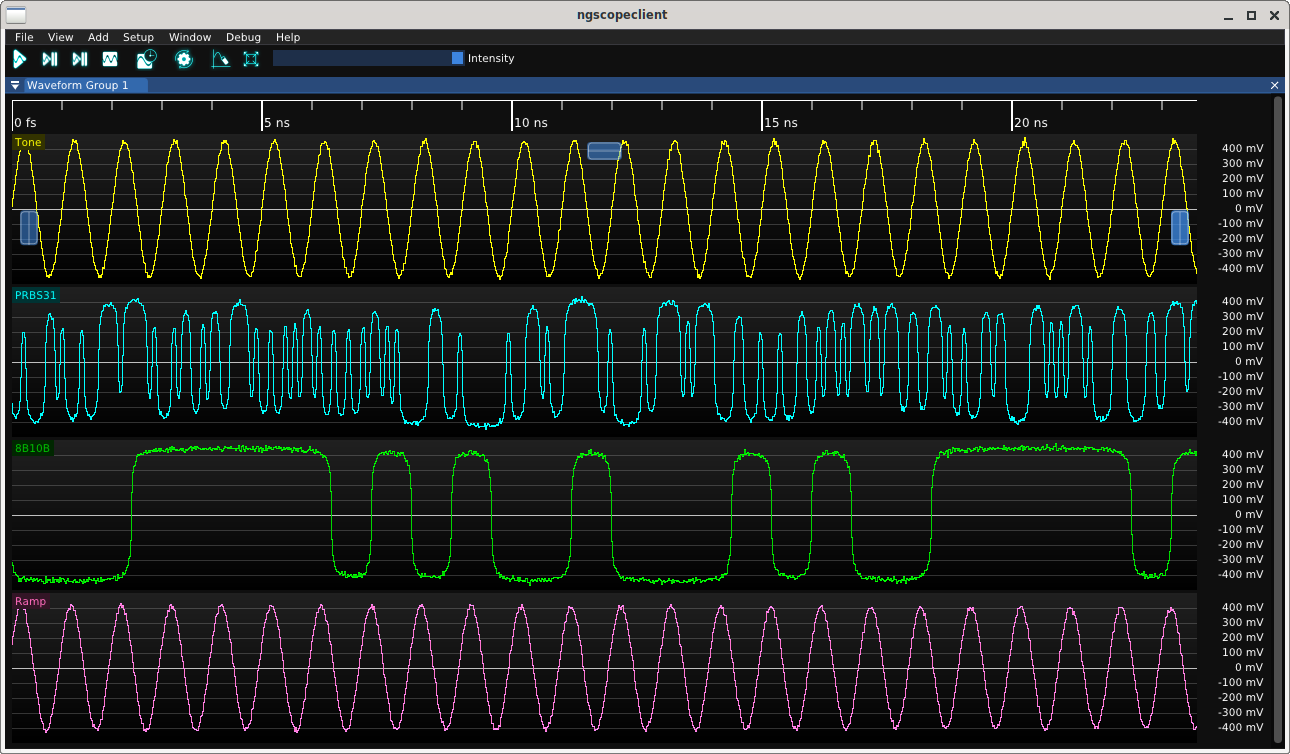
\includegraphics[width=13cm]{ng-images/split-overlays.png}
\caption{Overlays showing drag-and-drop locations for splitting waveform groups}
\label{split-overlays}
\end{figure}

\begin{figure}[h]
\centering
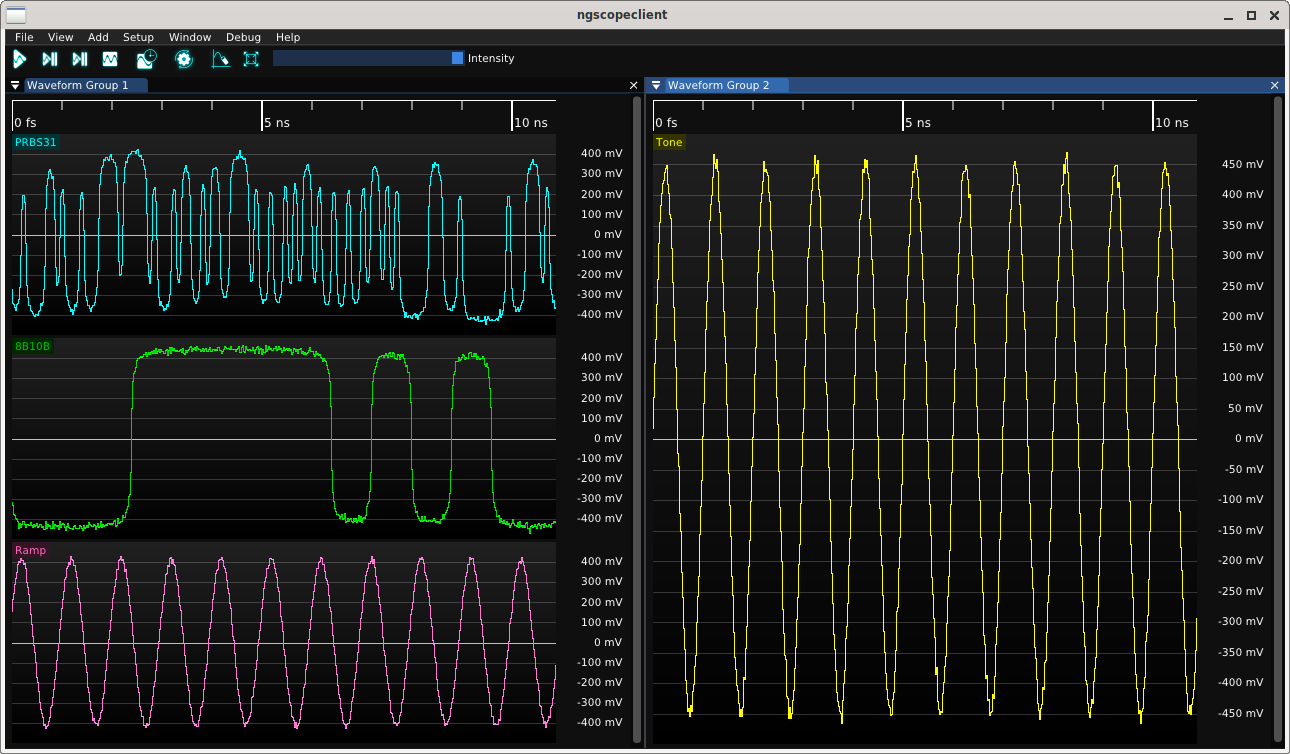
\includegraphics[width=13cm]{ng-images/split-right.png}
\caption{Result of dropping a waveform to the right side split area}
\label{split-right}
\end{figure}

Waveform groups may be resized arbitrarily by dragging the separator between them. The title bar of a group may also be
dragged, allowing the entire group to be undocked as a floating window. Floating windows can be re-docked by dragging
the title bar back into the main ngscopeclient window (or another floating window), creating new tabs or splitting
existing groups as desired (Fig. \ref{complex-ui}).

\begin{figure}[h]
\centering
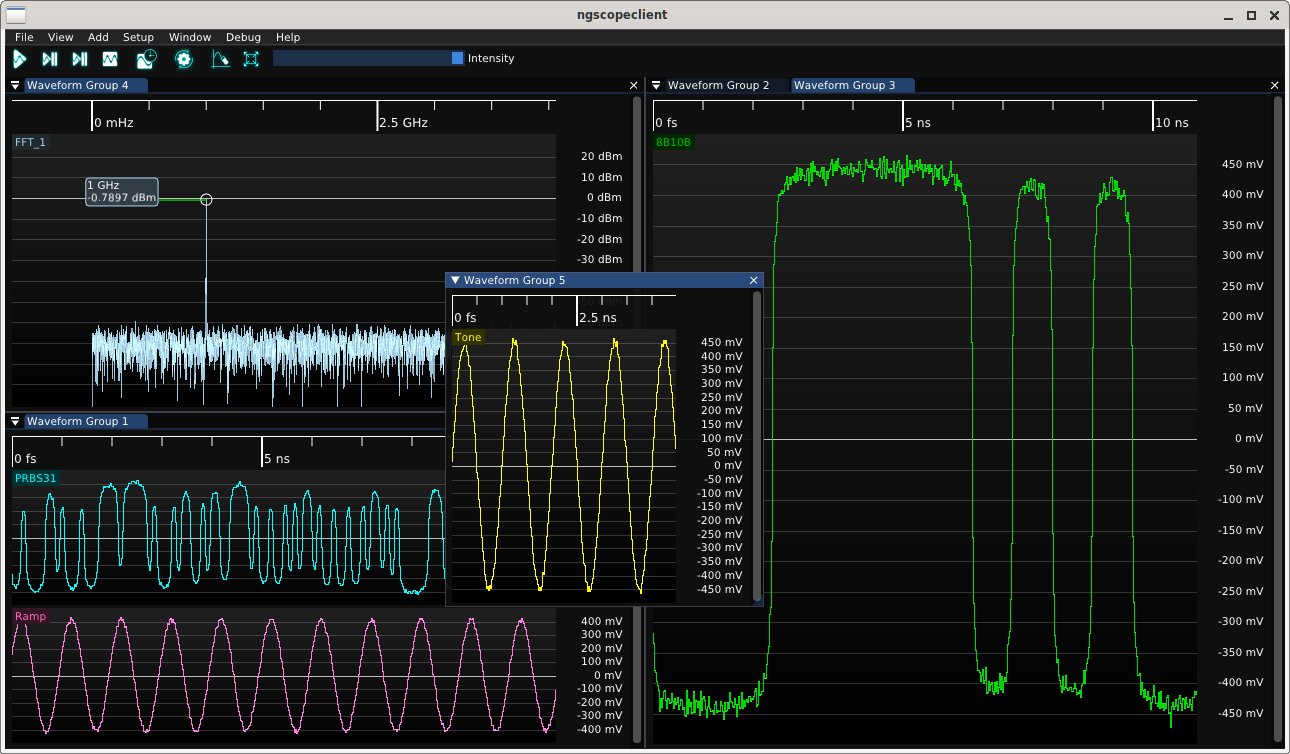
\includegraphics[width=13cm]{ng-images/complex-ui.png}
\caption{Example of complex window layout with multiple tabs, splitters between docked waveform groups, and a group in
a floating window}
\label{complex-ui}
\end{figure}

\chapter{Waveform Views}

A waveform view is a 2D graph of a signal or protocol decode within a waveform group.

Arbitrarily many channels of data may be displayed within a single view, however all analog channels within a single
view share the same Y axis unit, gain, and offset. Digital channels and protocol decodes can be overlaid on analog
waveforms or displayed in their own dedicated views.

2D density plots, such as eye patterns, spectrograms, and waterfall plots, cannot share a waveform view
with any other channel.

\section{Navigation}

Scrolling with the mouse wheel adjusts the horizontal scale of the current waveform group, zooming in or out centered
on the position of the mouse cursor.

%Pressing SHIFT while scrolling moves the view left and right without adjusting zoom. If your mouse has a horizontal
%scroll feature, this may also be used to pan without zooming.

%Pressing the middle mouse button auto-scales the active waveform group so that the entire waveform is visible.

\section{Plot Area}

The plot area shows the waveform being displayed. The horizontal grid lines line up with the voltage scale markings on
the Y axis. If the plot area includes Y=0, the grid line for zero is slightly brighter.

The waveform is drawn as a semi-transparent line so that when zoomed out, the density of voltage at various points in
the graph may be seen as lighter or darker areas. This is referred to as ``intensity grading".

\begin{figure}[H]
\centering
\includegraphics[width=10cm]{ng-images/graded-waveform.png}
\caption{Intensity-graded waveform}
\label{graded-waveform2}
\end{figure}

\section{Y Axis Scale}

Each waveform view has its own Y axis scale, which is locked to the ADC range of the instrument.

Channel gain may be configured by scrolling with the mouse wheel, and offset may be adjusted by dragging the scale with
the left mouse button. Pressing the middle mouse button on the Y axis will auto-scale the vertical gain and offset to
show the full span of all channels in the view with 5\% of vertical margin.

If a left-pointing arrow (as seen in Fig. \ref{y-axis}) is visible, one of the channels in the view is selected as a
trigger source. Click on the arrow and drag up or down to select the trigger level. Some trigger types, such as window
triggers, have two arrows for upper and lower levels.

\begin{figure}[H]
\centering
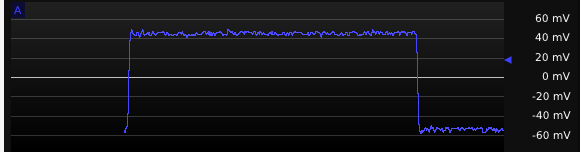
\includegraphics[height=3cm]{ng-images/y-axis.png}
\caption{Waveform view showing trigger arrow on Y axis}
\label{y-axis}
\end{figure}

\section{Channel Label}

The top left corner of each waveform view contains a legend with a label for each channel being displayed in the view.

Mousing over the channel name displays a tooltip (Fig. \ref{channel-tooltip}) with some helpful information about the
waveform. The exact information displayed in the tooltip depends on the type of data being displayed, for example
analog waveforms display sample rate and record length while eye patterns display the number of integrated UIs.

\begin{figure}[H]
\centering
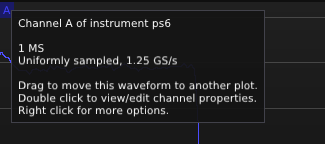
\includegraphics[height=3cm]{ng-images/channel-tooltip.png}
\caption{Example tooltip on channel label}
\label{channel-tooltip}
\end{figure}

The label may be dragged with the left mouse button to move the waveform to a different location. Dragging to the left
or right edge of a waveform view, or the top or bottom edge of the topmost or bottommost waveform in a group, will
split the group. Dragging to the left half of another waveform view, whether in the same group or a different group,
moves the channel to that view. Dragging to the right half of the view adds a new view within the same group containing
only the dragged waveform.

Double-clicking the label opens the channel properties dialog (Fig. \ref{channel-properties}). As with all dialogs in
ngscopeclient, the properties dialog may be left in the default floating state or docked.

\begin{figure}[H]
\centering
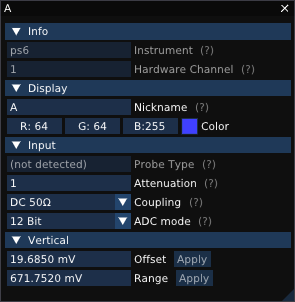
\includegraphics[height=5cm]{ng-images/channel-properties1.png}
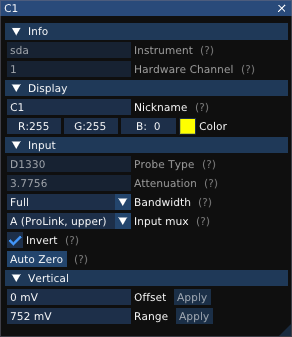
\includegraphics[height=5cm]{ng-images/channel-properties2.png}
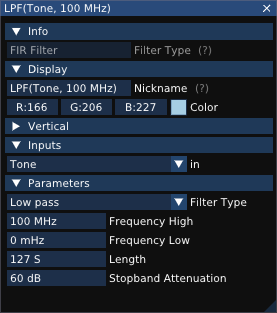
\includegraphics[height=5cm]{ng-images/channel-properties3.png}
\caption{Example of properties dialogs for three different channels}
\label{channel-properties}
\end{figure}

The properties dialog will always contain an editable nickname for the channel, a color chooser, and some basic
information about the instrument channel or filter block sourcing the data. Additional settings may be available but
will vary depending on the type of instrument or filter. In Fig. \ref{channel-properties}, the left dialog shows a
direct coaxial input to a Pico PicoScope 6824E, which has variable ADC resolution. The center dialog shows an active
differential probe with auto-zero capability, connected to a Teledyne LeCroy SDA816Zi-A which has a mux for selecting
between two input connectors for each channel. The right dialog shows a FIR filter with several configurable settings.

Right clicking on the label opens a context menu. The context menu allows setting of persistence mode, deleting the
waveform, and creating new filter blocks or protocol decodes with the selected waveform as an input.

\section{Cursors and Markers}
\label{sec:cursors}

Cursors are movable annotations which can be used to temporarily mark points of interest in a waveform and examine data
values. Markers are similar to cursors but intended for long-term marking of specific points in a single acquisition
and do not provide readout functionality.

\subsection{Vertical Cursors}

A vertical cursor describes a point in time \emph{relative to the start of the acquisition}. When new waveforms are
acquired, the cursor remains at the same offset in the new waveform. When the view is panned horizontally, the cursor
scrolls with the waveform and remains at the same point in the waveform.

To add a vertical cursor (Fig. \ref{vertical-cursor}), right click in the view and select a single or double cursor
from the \menustyle{Cursors | X Axis} menu.

Vertical cursors are attached to a waveform group and will span all views within the group. Multiple groups may have
independent vertical cursors active simultaneously.

\begin{figure}[H]
\centering
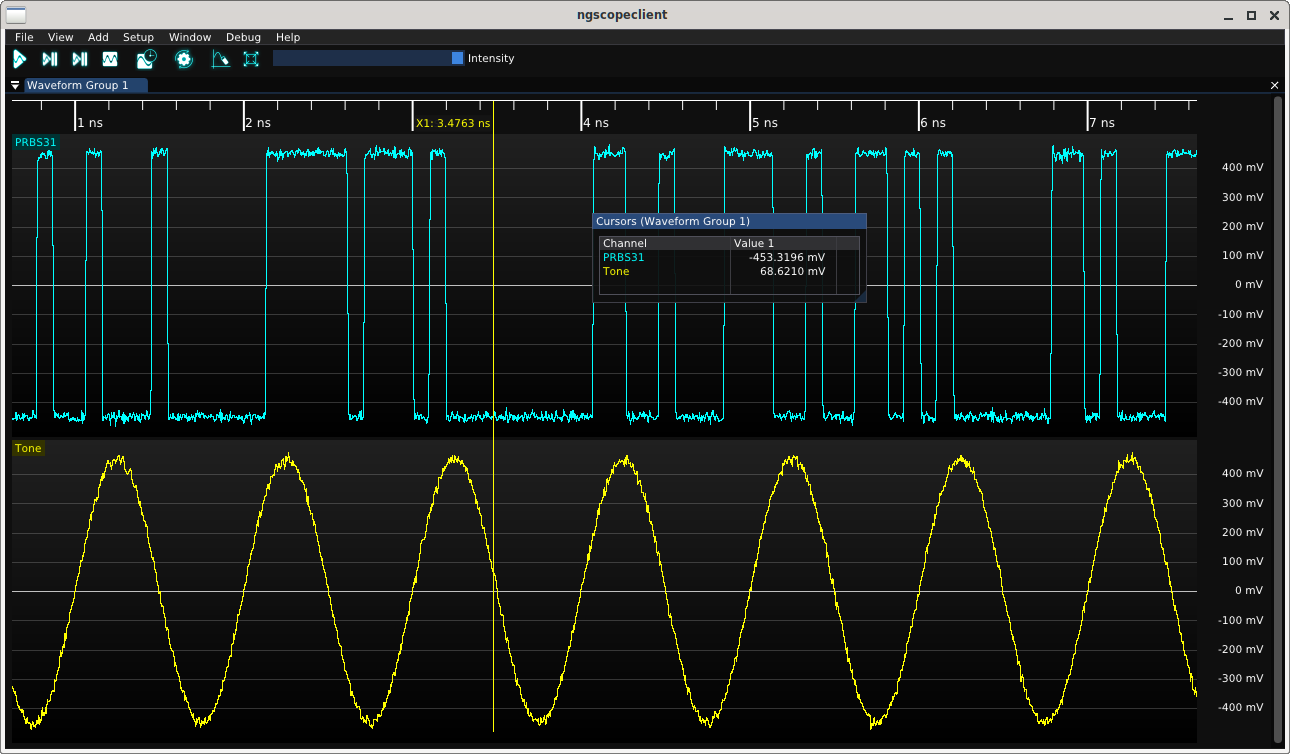
\includegraphics[width=13cm]{ng-images/vertical-cursor.png}
\caption{Single vertical cursor}
\label{vertical-cursor}
\end{figure}

\begin{figure}[H]
\centering
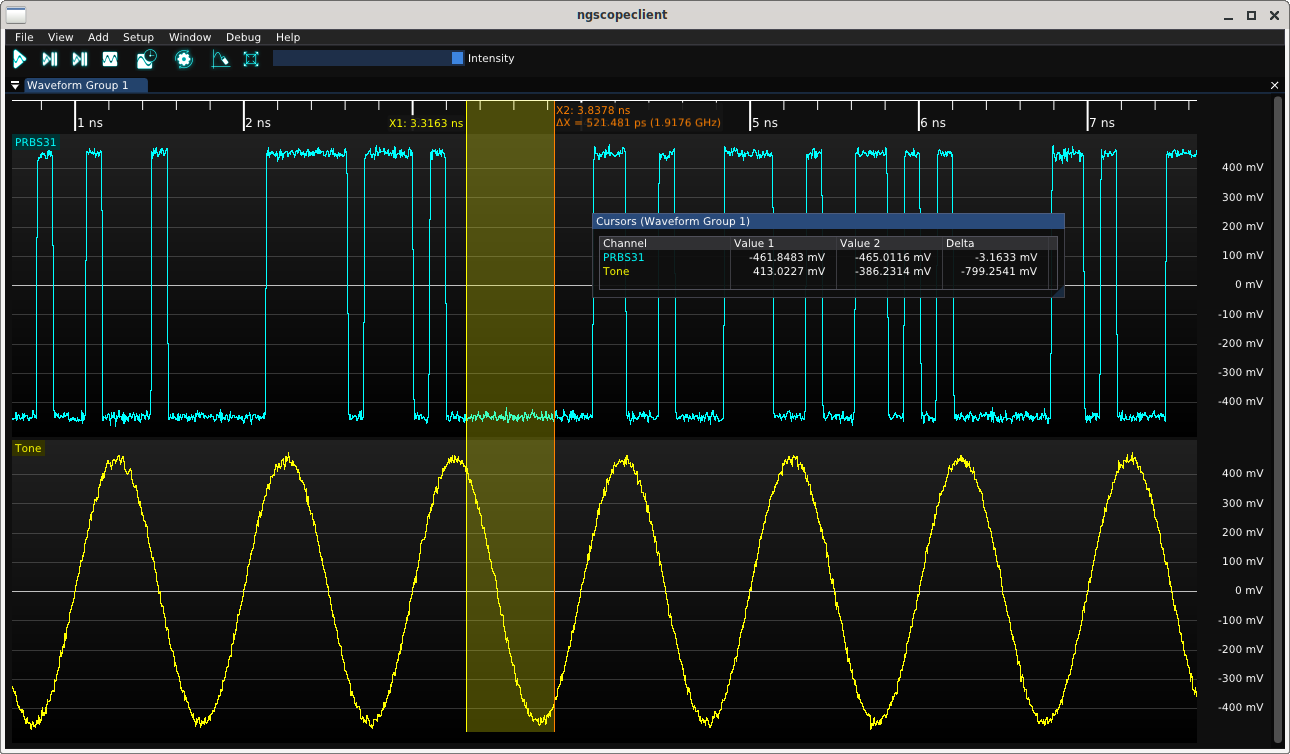
\includegraphics[width=13cm]{ng-images/vertical-cursor-x2.png}
\caption{Double vertical cursor}
\label{vertical-cursor-x2}
\end{figure}

To place a single cursor, click on the waveform at the desired location. To place double cursors, click at the starting
location to place the first cursor then drag to the ending location and release the mouse to place the second cursor.
Once placed, either cursor can be moved by clicking on it and dragging to the new location.

%Cursors will snap to transitions in digital signals or protocol decode overlays if the mouse is within a few pixels of
%the location. No snapping is applied when the mouse is over an analog waveform.

In the timeline each cursor will display its X-axis position. If both cursors are active, the delta between them
is shown. If the X axis uses time units, the frequency with period equal to the cursor spacing is also shown.

When a cursor is active, a dockable pop-up dialog appears displaying the value of each waveform in the group at the
cursor location. If two cursors are active, both values as well as the difference between them is shown (Fig.
\ref{vertical-cursor-x2})

%In FFT / spectrum analyzer plots, the integrated in-band power between both cursors is also shown.

\begin{comment}

If a protocol analyzer view (Chap. \ref{chapter:protoanalyzer}) is active, moving a single cursor over a packet will
scroll to and highlight that packet.

\end{comment}

\subsection{Markers}
\label{sec:markers}

A marker is a named location in \emph{absolute} time intended for marking specific events (such as protocol packets or
glitches) which may need to be re-examined in the future. When new waveforms are acquired, the marker remains attached
to the same point in the old waveform and will disappear until the old waveform is re-loaded from the history window.
In Fig. \ref{markers}, two of the three markers are visible while the third is in a prior waveform.

Unlike vertical cursors, which are local to a single waveform group, cursors are global and will appear at the same
timestamp in all waveform groups. This allows an event of interest to be examined in detail in one view, while a
different view provides a global overview of the entire acquisition or examines another event (Fig.
\ref{marker-multiview}).

Creating a marker automatically pins the active waveform so it will not be removed from history as new data is
acquired. The waveform cannot be un-pinned unless all markers are deleted first, or the waveform itself is manually
deleted.

Newly created markers will have default numeric names such as M1, M2, etc. This name can be changed from the history
window.

\begin{figure}[H]
\centering
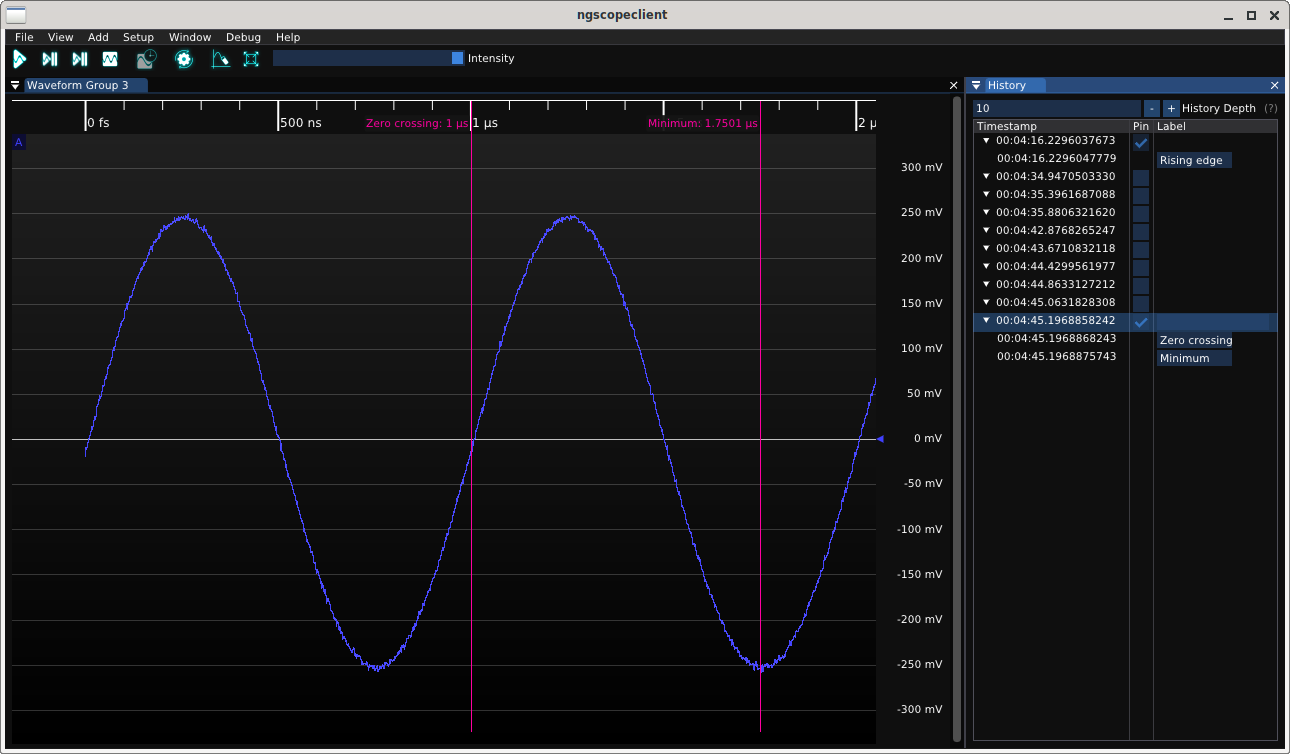
\includegraphics[width=13cm]{ng-images/markers.png}
\caption{Session with three markers, two on the currently displayed waveform and one on a prior waveform}
\label{markers}
\end{figure}

\begin{figure}[H]
\centering
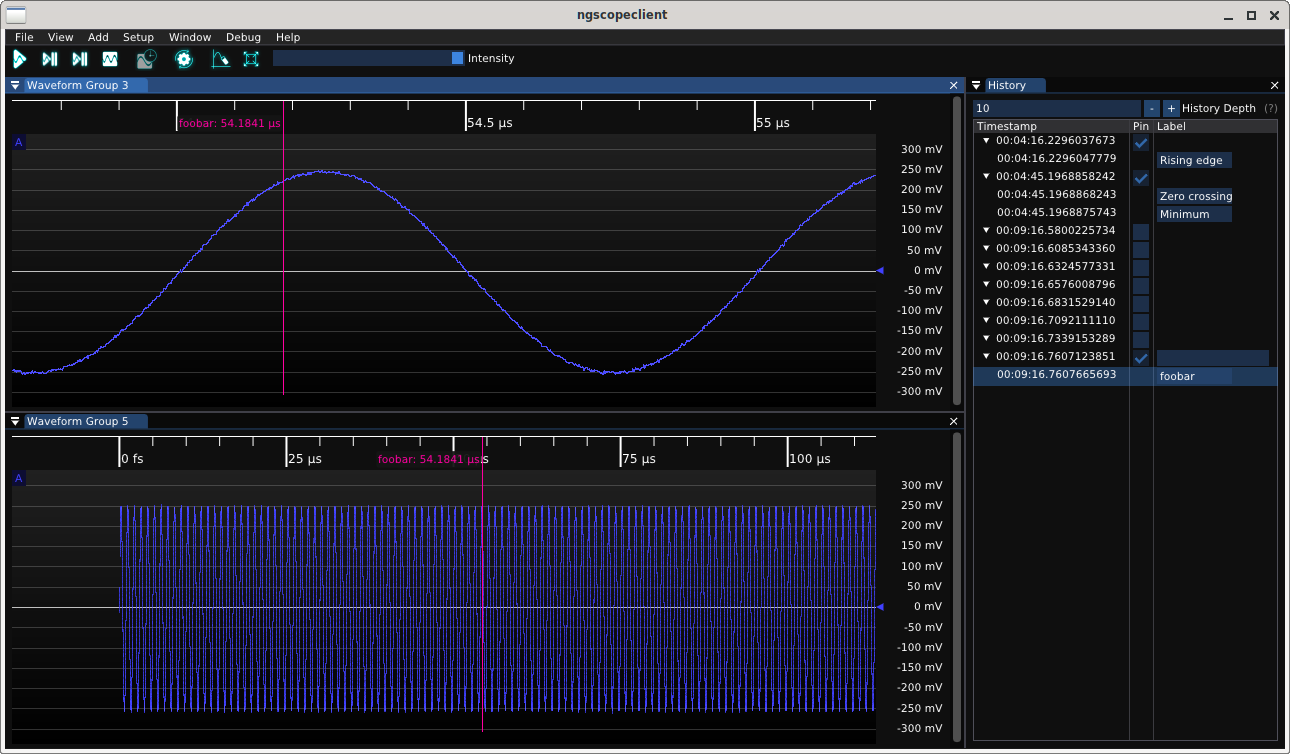
\includegraphics[width=13cm]{ng-images/marker-multiview.png}
\caption{A single marker seen at multiple time scales in different views}
\label{marker-multiview}
\end{figure}


\begin{comment}

\subsection{Horizontal Cursors}

To add a horizontal cursor (Fig. \ref{horizontal-cursor}), right click on the waveform and select \menustyle{Cursor |
Horizontal (single)} or \menustyle{Cursor | Horizontal (dual)} as appropriate.

\begin{figure}[H]
\centering
\includegraphics[width=8cm]{images/horizontal-cursor.png}
\caption{Horizontal cursor}
\label{horizontal-cursor}
\end{figure}

To place a single cursor, click on the waveform at the desired location. To place double cursors, click at the starting
location to place the first cursor then drag to the ending location and release the mouse to place the second cursor.
Once placed, either cursor can be moved by clicking on it and dragging to the new location.

At the right side of the plot, each cursor will display its Y-axis location. If both cursors are active, the delta
between them is also shown.

All waveform areas in a group share the same Y axis cursor positions.
\end{comment}

\chapter{History}
\label{sec:history}

ngscopeclient saves a rolling buffer of previous waveforms in memory, allowing you to go back in time and see previous
state of the system being debugged. Clicking on a timestamp in the history view (Fig. \ref{historyview}) pauses
acquisition and loads the historical waveform data for analysis. History is captured regardless of whether the window
is visible or not.

\begin{figure}[H]
\centering
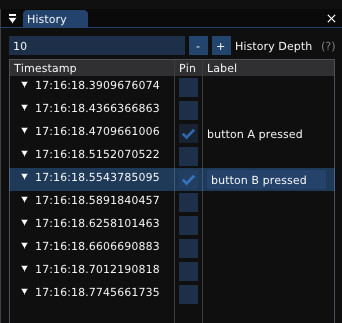
\includegraphics[width=7cm]{ng-images/history.png}
\caption{Waveform history view}
\label{historyview}
\end{figure}

The history depth defaults to 10 waveforms, but can be set arbitrarily within the limits of available RAM. Older
waveforms beyond the history limit are deleted as new waveforms are acquired. Any single waveform in history may also
be deleted by right clicking on the line and selecting ``delete" from the menu.

%The status bar at the bottom of the history view displays the total number of waveforms in the history, as well as an
%estimate of the amount of RAM used by the history.

\section{Pinning}

Interesting waveforms may be ``pinned" in the history by checking the box in the ``pin" column of the history view.
Pinned waveforms are guaranteed to remain in the history buffer even when new waveforms arrive; only unpinned waveforms
are eligible for automatic deletion to make space for incoming data.

If a waveform contains markers (\ref{sec:markers}), it is automatically pinned and cannot be unpinned unless the
marker (or entire waveform) is deleted. This prevents accidental loss of an important waveform: if the event was
important enough to mark and name, it is probably worth keeping around.

\section{Labeling}

Arbitrary text names may be assigned to a waveform by clicking the corresponding cell in the ``label" column.
Waveforms with a label are automatically pinned, since assigning a label implies the waveform is important.

\begin{comment}

\section{Estimating Waveform Memory Usage}

When selecting a maximum depth for the history, it is important to pick a reasonable limit to avoid running out of RAM!
ngscopeclient will happily fill tens or hundreds of gigabytes of memory with deep waveforms if given a chance. Memory
usage of waveform data can be roughly estimated as 16 + sizeof(sample type) bytes per point, since each sample contains a
64-bit timestamp and duration plus the sample data.

For example, an analog sample takes 20 bytes of RAM (16 of time plus a 32-bit floating point voltage measurement) per
sample. Thus, a 1M point analog waveform takes approximately 20 MB of RAM per channel, or 80 MB per capture on a
four-channel oscilloscope with all channels enabled.

On the larger side, a 10M point four channel capture would use 800 MB and a 64M point deep-memory capture would use 5
GB. A deep history setting, such as 100 waveforms, is thus wildly inappropriate for such deep captures! A future
software release may support spilling waveform data to a temporary directory on disk, permitting effectively unlimited
history depth given sufficient disk space.

Digital waveforms use one byte per sample for the actual measurement, so 17 MB per channel for a 1M point waveform.
Most logic analyzer or MSO drivers for libscopehal will perform automatic de-duplication when a waveform goes several
clock cycles with no toggles, so the actual memory usage is likely to be significantly less than this.

Filter memory usage varies depending on the specific filter in question, however it is typically not a large
contributor to the overall ngscopeclient RAM footprint when using history mode because filters are evaluated
dynamically each time a waveform is pulled from history rather than having output cached for every historical waveform.
Thus, at most one copy of each filter's output is present in memory regardless of history depth.
\end{comment}

\chapter{Filter Graph Editor}
\label{grapheditor}

\section{Introduction}

The filter graph editor allows complex signal processing pipelines to be developed in a graphical fashion. It may be
accessed from the \menustyle{Window | Filter Graph} menu item.

The graph editor view (Fig. \ref{graph-editor}) shows nodes for every instrument channel, trigger, and filter block in
the current session. As new instruments, channels, and filter blocks are added to the session, new nodes will
automatically appear in the graph editor view. Nodes cannot overlap and will automatically move out of the way if
another node is dragged on top of them.

\begin{figure}[H]
\centering
\bigimage{ng-images/graph-editor.png}
\caption{Filter graph editor showing instrument channels and several processing blocks}
\label{graph-editor}
\end{figure}

\section{Interaction}

The view may be zoomed with the mouse wheel, or panned by dragging with the right mouse button, to navigate large
filter graphs which do not fit on a single screen at a reasonable zoom level. Right clicking on a node opens a pop-up
properties view (Fig. \ref{graph-editor-properties}).

\begin{figure}[H]
\centering
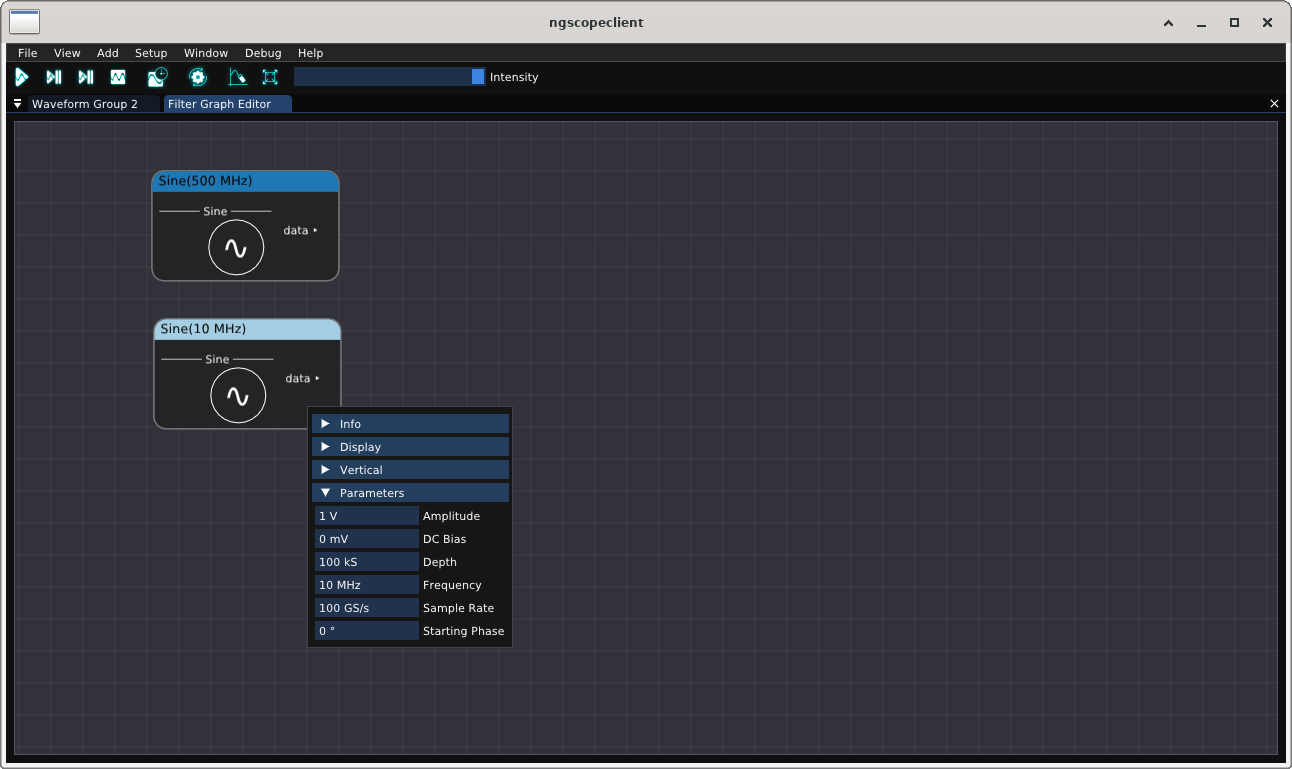
\includegraphics[width=8cm]{ng-images/graph-editor-properties.png}
\caption{Filter graph editor showing properties popup}
\label{graph-editor-properties}
\end{figure}

Nodes display inputs at left and outputs at right. To connect two existing nodes, click on an input or output port and
drag to the port you wish to connect it to. An input can only connect to one output at a time; if the destination
already is connected to a different signal the previous connection will be removed and replaced with the new one.

A tooltip with a green plus sign is displayed during dragging if the proposed connection is valid. If the tooltip
displays a red X instead, the connection is invalid (connecting two inputs, two outputs, or an input and output of
incompatible data types).

To create a new node, click on an input or output port and drag to an empty area of the canvas (Fig.
\ref{graph-editor-create}, Fig. \ref{graph-editor-addinput}). A context menu will appear, presenting a list of filters
which can accept (if dragging from an output) or produce (if dragging from an input) the desired data type. If dragging
from an input, the context menu will also include any currently unused instrument channels.

\begin{figure}[H]
\centering
\bigimage{ng-images/graph-editor-create.png}
\caption{Filter graph editor dragging from an output to an empty area of the canvas}
\label{graph-editor-create}
\end{figure}

\begin{figure}[H]
\centering
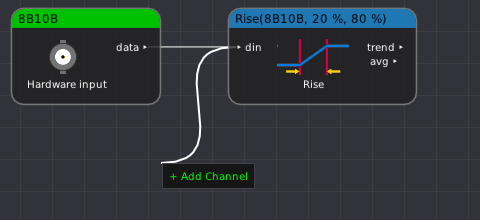
\includegraphics[width=10cm]{ng-images/graph-editor-addinput.png}
\caption{Filter graph editor dragging from an input to an empty area of the canvas}
\label{graph-editor-addinput}
\end{figure}

When a new node is added to the filter graph, each output channel will be automatically added to an existing waveform
view if a compatible one is present. If no compatible view is available, a new view and/or group will be created.

Node title bars are color-coded to match the display color of the waveform trace, allowing easy navigation between
waveform views and the graph editor.

Each node also includes a caption stating the type of node (``hardware input", ``hardware output", or the name of the
filter block) and, in most cases, an icon depicting the functionality of the block.\footnote{Not all filters currently
have icons. We are working with multiple artists to create more filter icons and welcome additional contributions.}

\section{Grouping}

In order to better organize complex experimental setups, nodes may be organized in groups. Groups cannot be nested.

To create a group, right click an unused area of the graph editor canvas and select ``New Group" from the context menu.
This will spawn a new, empty group near the mouse cursor position.

The group will have an automatically generated name (Fig. \ref{graph-editor-group1}) by default. This name may be
changed by right clicking on the group's title bar and typing a new name in the pop-up.

\begin{figure}[H]
\centering
\bigimage{ng-images/graph-editor-group1.png}
\caption{Newly created node group}
\label{graph-editor-group1}
\end{figure}

To add a node to a group, simply drag the node by its title bar and move it into the group (Fig.
\ref{graph-editor-group2}). All paths from the node to the remainder of the filter graph will be routed through
``hierarchical ports" at the left and right edges of the group, reducing clutter. Nodes may be freely moved around
within the group to organize them, or dragged out of the group to remove them from the group.

A group (together with its contents) may be moved by dragging the group's title bar with the left mouse button, or
resized by dragging any of its corners. When a group is moved, it will push other nodes or groups out of the way to
prevent overlapping.

If not needed, a group can be deleted by selecting it with the left mouse button and pressing the ``delete" key.
Deleting a group does not remove any nodes contained within it.

\begin{figure}[H]
\centering
\bigimage{ng-images/graph-editor-group2.png}
\caption{Groups containing several nodes with hierarchical ports}
\label{graph-editor-group2}
\end{figure}

\chapter{Transports}
\label{sec:transports}

Libscopehal uses a ``transport" object in order to pass commands and data to instruments, in order to decouple the
specifics of LXI, USBTMC, etc. from individual instrument drivers. This section describes the supported transports and
their usage and limitations.

Not all transports are possible to use with any given driver due to hardware limitations or software/firmware quirks.
For details on which transport(s) are usable with a particular instrument, consult the documentation for that device's
driver.

\section{gpib}

SCPI over GPIB.

This transport takes up to four arguments: GPIB board index, primary address, secondary address, and timeout value.
Only board index and primary address are required. We currently support using a single GPIB device per GPIB board 
(interface) in a ngscopeclient session. You cannot currently access multiple devices in the same or across instances.
Better support for multiple instrument on a single board is planned.

NOTE: The current implementation of this driver only works on Linux, using the linux-gpib library.

Example:
\begin{lstlisting}[language=sh, numbers=none]
ngscopeclient myscope:keysightdca:gpib:0:7
\end{lstlisting}

\section{lan}

SCPI over TCP with no further encapsulation.

This transport takes two arguments: hostname/IP and port number.

If port number is not specified, uses TCP port 5025 (IANA assigned) by default. Note that Rigol oscilloscopes use the
non-standard port 5555, not 5025, so the port number must always be specified when using a Rigol instrument.

Example:
\begin{lstlisting}[language=sh, numbers=none]
ngscopeclient myscope:rigol:lan:192.0.2.9:5555
\end{lstlisting}

\section{lxi}

SCPI over LXI VXI-11.

Note that due to the remote procedure call paradigm used by LXI, it is not possible to batch multiple outstanding
requests to an instrument when using this transport. Some instruments may experience reduced performance when using LXI
as the transport. Drivers which require command batching may not be able to use LXI VXI-11 as the transport even if the
instrument supports it.

Example:
\begin{lstlisting}[language=sh, numbers=none]
ngscopeclient myscope:tektronix:lxi:192.0.2.9
\end{lstlisting}

\section{null}

This transport does nothing, and is used as a placeholder for development simulations or non-SCPI instruments.

NOTE: Due to limitations of the current command line argument parsing code, an argument must be provided to all
transports, including this one, when connecting via the command line. Since the argument is ignored, any non-empty
string may be used.

Example:
\begin{lstlisting}[language=sh, numbers=none]
ngscopeclient sim:demo:null:blah
\end{lstlisting}

\section{twinlan}

This transport is used by some Antikernel Labs oscilloscopes, as well as most of the bridge servers used for interfacing
libscopehal with USB oscilloscopes' SDKs. It takes three arguments: hostname/IP and two port numbers.

It uses two TCP sockets on different ports. The first carries SCPI text (as in the ``lan" transport), and the second is
for binary waveform data.

If port numbers are not specified, the SCPI port defaults to the IANA standard of 5025, and the data port defaults to
5026. If the SCPI port but not the data port is specified, the data port defaults to the SCPI port plus one.

\section{uart}

SCPI over RS-232 or USB-UART.

This transport takes two arguments: device path (required) and baud rate (optional). If baud rate is not specified, it
defaults to 115200.

Example:
\begin{lstlisting}[language=sh, numbers=none]
ngscopeclient myscope:rigol:uart:/dev/ttyUSB0:115200
\end{lstlisting}

\section{usbtmc}

SCPI over USB Test \& Measurement Class protocol.

This transport takes one argument: the path to the usbtmc kernel device object.

NOTE: The current implementation of this driver only works on Linux. There is currently no support for USBTMC on
Windows (\issue{scopehal}{301})

Example:
\begin{lstlisting}[language=sh, numbers=none]
ngscopeclient myscope:siglent:usbtmc:/dev/usbtmc0
\end{lstlisting}

\section{vicp}

SCPI over Teledyne LeCroy Virtual Instrument Control Protocol.

This transport takes two arguments: hostname/IP and port number.

If port number is not specified, uses TCP port 1861 (IANA assigned) by default.

Example:
\begin{lstlisting}[language=sh, numbers=none]
ngscopeclient myscope:lecroy:vicp:192.0.2.9
\end{lstlisting}



\chapter{BERT Drivers}
\label{sec:bert-drivers}

This chapter describes all of the available drivers for bit error rate testers (BERTs)

\section{Antikernel Labs}

\begin{tabularx}{16cm}{lllX}
\thickhline
\textbf{Device Family} & \textbf{Driver} & \textbf{Transport} & \textbf{Notes} \\
\thickhline
AKL-TXB1 & akl.crossbar & lan &  \\
\thickhline
\end{tabularx}

\subsection{akl.crossbar}

This is the driver for the \href{https://github.com/azonenberg/trigger-crossbar}{AKL-TXB1} trigger crossbar and CDR
trigger system. The front panel transceiver ports can also be used as a BERT.

\section{MultiLANE}

\begin{tabularx}{16cm}{lllX}
\thickhline
\textbf{Device Family} & \textbf{Driver} & \textbf{Transport} & \textbf{Notes} \\
\thickhline
ML4039-BTP & mlbert & lan & Use \href{https://github.com/ngscopeclient/scopehal-mlbert-bridge}{scopehal-mlbert-bridge} \\
\thickhline
\end{tabularx}

\subsection{mlbert}

This driver is intended to connect via the
\href{https://github.com/ngscopeclient/scopehal-mlbert-bridge}{scopehal-mlbert-bridge} server for network transparency
and does not directly link to the MultiLANE SDK or talk directly to the instrument. The bridge requires a Windows PC
since MultiLANE's SDK is Windows only, however the libscopehal clientside driver can run on any supported OS.

It was developed using a ML4039-BTP but may work with other similar models as well.

\chapter{Function Generator Drivers}
\label{sec:funcgen-drivers}

This chapter describes all of the available drivers for standalone function generators.

Function generators which are part of an oscilloscope are described in the \hyperref[sec:scope-drivers]{Oscilloscope
Drivers} section.

\section{Rigol}

\begin{tabularx}{16cm}{lllX}
\thickhline
\textbf{Device Family} & \textbf{Driver} & \textbf{Transport} & \textbf{Notes} \\
\thickhline
DG4000 series & rigol\_awg & lan & Only tested via lan transport, but USBTMC and serial are available too\\
\thickhline
\end{tabularx}

\subsection{rigol\_awg}

This driver supports all DG4000 series function / arbitrary waveform generators.


\chapter{Electronic Load Drivers}
\label{sec:load-drivers}

This chapter describes all of the available drivers for electronic loads.

\section{Siglent}

\begin{tabularx}{16cm}{lllX}
\thickhline
\textbf{Device Family} & \textbf{Driver} & \textbf{Transport} & \textbf{Notes} \\
\thickhline
SDL1000X/X-E series & siglent\_load & lan & Only tested via lan transport, but USBTMC and serial are available too\\
\thickhline
\end{tabularx}

\subsection{siglent\_load}

This driver supports all SDL1000 family loads (SDL1020X-E, SDL1020X, SDL1030X-E, SDL1030X).

\chapter{Multimeter Drivers}
\label{sec:meter-drivers}

This chapter describes all of the available drivers for multimeters.

Multimeters which are part of an oscilloscope are described in the \hyperref[sec:scope-drivers]{Oscilloscope
Drivers} section.

\section{Rohde \& Schwarz}

\begin{tabularx}{16cm}{lllX}
\thickhline
\textbf{Device Family} & \textbf{Driver} & \textbf{Transport} & \textbf{Notes} \\
\thickhline
HMC8012 & rs\_hmc8012 & lan & Only tested via lan transport, but USBTMC and serial are available too\\
\thickhline
\end{tabularx}

\subsection{rs\_hmc8012}

This driver supports the HMC8012 multimeter, which is the only device in the family.

\chapter{Miscellaneous Drivers}
\label{sec:misc-drivers}

This chapter describes all of the available drivers for miscellaneous instruments which do not fit in any other
category.

\section{Generic}

\begin{tabularx}{16cm}{lllX}
\thickhline
\textbf{Device Family} & \textbf{Driver} & \textbf{Transport} & \textbf{Notes} \\
\thickhline
N/A & csvstream & Any & \\
\thickhline
\end{tabularx}

\subsection{csvstream}

This driver exposes the most recent line from a stream of comma-separated value (CSV) data as a series of analog scalar
channels.

It is primarily intended for extracting low rate I2C sensor readings and ADC values from an embedded DUT, so that that
these values may be plotted alongside multimeter/power supply readings or other data coming from more conventional
instrumentation.

The data may come from any supported transport, however it is expected that the most likely scenario is either direct
connection to a local serial port (``uart" transport), or a TCP socket connected to either a remote UART using socat or
an embedded TCP server (``lan" transport).

Data must be generally line oriented and UTF-8 or 7-bit ASCII encoded.

In order to enable csvstream data to share a UART also used by other traffic such as a debug console or syslog, all
lines must contain one of three magic prefixes as shown below. Any content in the line before the prefix (such as a
timestamp) is ignored.

Upon initial connection, the driver will have a single channel called ``CH1". At any time, if the number of fields in a
received CSV line exceeds the current channel count, a new channel will be created. If a partial line is received, the
values in the missing columns are unchanged but the channel will not be deleted.

\begin{itemize}
\item \textbf{CSV-NAME}: Contains channel name data. Example:\\
CSV-NAME,Temperature,3V3,RxLevel

\item \textbf{CSV-UNIT}: Contains channel unit data (using the text encodings used by the libscopehal Unit class). Example:\\
CSV-UNIT,°C,V,dBm

\item \textbf{CSV-UNIT}: Contains channel value data. Example:\\
CSV-DATA,31.41,3.291,-59.1

\end{itemize}

\chapter{Oscilloscope Drivers}
\label{sec:scope-drivers}

This chapter describes all of the available drivers for oscilloscopes and logic analyzers.

\section{Agilent}

Agilent devices support a similar similar SCPI command set across most device families.

Please see the table below for details of current hardware support:

\begin{tabularx}{16cm}{lllX}
\thickhline
\textbf{Device Family} & \textbf{Driver} & \textbf{Transport} & \textbf{Notes} \\
\thickhline
DSO5000 series & agilent & lan & Not recently tested, but should work.\\
\thinhline
DSO6000 \& MSO6000 series & agilent & lan &  Working. No support for digital channels yet.\\
\thinhline
DSO7000 \& MSO7000 series & agilent & lan & Untested, but should work. No support for digital channels yet.\\
\thinhline
MSOX-2000 series & agilent & lan \\
\thinhline
MSOX-3000 series & agilent & lan \\
\thickhline
\end{tabularx}

\subsection{agilent}

\subsubsection{Typical Performance (MSO6034A, LAN)}

Interestingly, performance sometimes gets better with more channels or deeper memory. Not sure why.

\begin{tabularx}{16cm}{llX}
\thickhline
\textbf{Channels} & \textbf{Memory depth} & \textbf{WFM/s}\\
\thickhline
1 & 1K & 66 \\
\thinhline
4 & 1K & 33 \\
\thinhline
4 & 4K & 33 \\
\thinhline
1 & 40K & 33 \\
\thinhline
1 & 4K & 22 \\
\thinhline
1 & 20K & 22 \\
\thinhline
4 & 20K & 22 \\
\thinhline
1 & 100K & 22 \\
\thinhline
4 & 10K & 17 \\
\thinhline
4 & 40K & 12 \\
\thinhline
1 & 200K & 11 \\
\thinhline
1 & 400K & 8 \\
\thinhline
4 & 100K & 6.5 \\
\thinhline
4 & 200K & 4 \\
\thinhline
1 & 1M & 3.7 \\
\thinhline
4 & 400K & 2.3 \\
\thinhline
1 & 1M & 1 \\
\thinhline
4 & 1M & 1 \\
\thinhline
4 & 4M & 0.2 \\
\thickhline
\end{tabularx}

\subsubsection{Typical Performance (MSOX3104T, LAN)}

\begin{tabularx}{16cm}{llX}
\thickhline
\textbf{Channels} & \textbf{Memory depth} & \textbf{WFM/s}\\
\thickhline
1 & 2.5K & 3.3 \\
\thinhline
4 & 2.5K & 2.5 \\
\thinhline
1 & 2.5M & 1.0 \\
\thinhline
4 & 2.0M & 0.5 \\
\thickhline
\end{tabularx}

\section{Antikernel Labs}

\begin{tabularx}{16cm}{llX}
\thickhline
\textbf{Device Family} & \textbf{Driver} & \textbf{Notes} \\
\thickhline
Internal Logic Analyzer IP & akila & \\
\thickhline
BLONDEL Oscilloscope Prototype & aklabs & \\
\thickhline
\end{tabularx}

\subsection{akila}

This driver uses a raw binary protocol, not SCPI.

Under-development internal logic analyzer analyzer core for FPGA design debug. The ILA uses a UART interface to a host
system. Since there's no UART support in scopehal yet, socat must be used to bridge the UART to a TCP socket using
the ``lan" transport.

\subsection{aklabs}

This driver uses two TCP sockets. Port 5025 is used for SCPI control plane traffic, and port 50101 is used for waveform
data using a raw binary protocol.

\section{Demo}

The ``demo" driver is a simulation-only driver for development and training purposes, and does not connect to real
hardware.

It ignores any transport provided, and is normally used with the ``null" transport.

The demo instrument is intended to illustrate the usage of ngscopeclient for various types of analysis and to aid in
automated testing on computers which do not have a connection to a real oscilloscope, and is not intended to accurately
model the response or characteristics of real world scope frontends or signals.

It supports memory depths of 10K, 100K, 1M, and 10M points per waveform at rates of 1, 5, 10, 25, 50, and 100 Gsps.
Four test signals are provided, each with 10 mV of Gaussian noise and a 5 GHz low-pass filter added (although this can
be disabled under the channel properties)

Test signals:
\begin{itemize}
\item 1.000 GHz tone
\item 1.000 GHz tone mixed with a second tone, which sweeps from 1.100 to 1.500 GHz
\item 10.3125 Gbps PRBS-31
\item 1.25 Gbps repeating two 8B/10B symbols (K28.5 D16.2)
\end{itemize}

\begin{tabularx}{16cm}{lllX}
\thickhline
\textbf{Device Family} & \textbf{Driver} & \textbf{Transport} & \textbf{Notes} \\
\thickhline
Simulator & demo & null & \\
\thickhline
\end{tabularx}

\section{Digilent}

Digilent oscilloscopes using the WaveForms SDK are all supported using the ``digilent" driver in libscopehal. This
driver connects using the ``twinlan" transport to a \href{https://github.com/glscopeclient/scopehal-waveforms-bridge}
{socket server} which links against the Digilent WaveForms SDK. This provides network transparency, and allows the
Digilent bridge server to be packaged separately for distribution and only installed by users who require it.

As of 2022-03-09, analog input channels on the Analog Discovery Pro and Analog Discovery 2 have been tested and are
functional, however only basic edge triggering is implemented so far. Analog inputs on other devices likely work,
however only these two have been tested to date.

Analog outputs, digital inputs, and digital outputs are currently unimplemented, but are planned to be added in the
future.

\subsection{digilent}

\begin{tabularx}{16cm}{lllX}
\thickhline
\textbf{Device Family} & \textbf{Driver} & \textbf{Transport} & \textbf{Notes} \\
\thickhline
Electronics Explorer & digilent & twinlan & Not tested, but probably works\\
\thinhline
Analog Discovery & digilent & twinlan & Not tested, but probably works\\
\thinhline
Analog Discovery 2 & digilent & twinlan & No digital channel support \newline No analog output support\\
\thinhline
Analog Discovery Pro & digilent & twinlan & No digital channel support \newline No analog output support \\
\thinhline
Digital Discovery & digilent & twinlan & No digital channel support,\newline so pretty useless for now\\
\thickhline
\end{tabularx}

\subsubsection{Typical Performance (ADP3450, USB -> LAN)}

\begin{tabularx}{16cm}{llX}
\thickhline
\textbf{Channels} & \textbf{Memory depth} & \textbf{WFM/s}\\
\thickhline
4 & 64K & 25.8 \\
\thinhline
2 & 64K & 32.3 \\
\thinhline
1 & 64K & 33.0 \\
\thickhline
\end{tabularx}

\section{DreamSource Lab}

DreamSourceLabs oscilloscopes and logic analyzers supported in their fork of sigrok (``libsigrok4DSL'' distributed as part of
their ``DSView'' software package) are supported through the ``dslabs'' driver in libscopehal. This driver connects using
the ``twinlan'' transport to a \href{https://github.com/glscopeclient/scopehal-sigrok-bridge}{socket server} which links
against libsigrok4DSL. This provides network transparency, and allows the DSLabs bridge server to be packaged separately for
distribution and only installed by users who require it.

As of 2022-03-22, a DSCope U3P100 and a DSLogic U3Pro16has been tested and works adequately. Other products may work
also, but are untested.

On DSCope: Only edge triggers are supported. `Any' edge is not supported. ``Ch0 \&\& Ch1'' and ``Ch0 || Ch1'' trigger modes
are not supported.

On DSLogic: Only edge triggers are supported. All edges are supported. There is currently no way to configure a trigger on more
than one channel. Serial / multi-stage triggers are not supported.

Known issues pending fixes/refactoring:
\begin{itemize}
	\item Interleaved sample rates are not correctly reported in the timebase dialog (but are in the waveform display)
	\item Trigger position is quantized to multiples of 1\% of total capture
	\item Non-localhost performance, and responsiveness in general may suffer as a result of hacky flow control on waveform capture
	\item DSLogic depth configuration is confusing and performance could be improved (currently only buffered more is supported)
	\item DSLogic devices trigger even if pre-trigger buffer has not been filled, leading to a small pre-trigger waveform in some cases
\end{itemize}

\subsection{dslabs}

\begin{tabularx}{16cm}{lllX}
\thickhline
\textbf{Family / Device} & \textbf{Driver} & \textbf{Transport} & \textbf{Notes} \\
\thickhline
DSCope U3P100 & dslabs & twinlan & Tested, works\\
\thinhline
DSLogic U3P16 & dslabs & twinlan & Tested, works\\
\thinhline
DSCope (others) & dslabs & twinlan & Not tested, but probably works\\
\thinhline
DSLogic (others) & dslabs & twinlan & Not tested, but probably works\\
\thickhline
\end{tabularx}

\subsubsection{Typical DSCope Performance (DSCope U3P100, USB3, localhost)}

\begin{tabularx}{16cm}{lllXX}
\thickhline
\textbf{Channels} & \textbf{Memory depth} & \textbf{Sample Rate} & \textbf{WFM/s} & \textbf{UI-unconstrained WFM/s}\\
\thickhline
2 & 1M & 100MS/s & 14 & 50\\
\thinhline
2 & 5M & 500MS/s & 4.5 & 14\\
\thinhline
1 & 5M & 1GS/s & 8.3 & 32\\
\thickhline
\end{tabularx}

\subsubsection{Typical DSLogic Performance (DSLogic U3Pro16, USB3, localhost)}

\begin{tabularx}{16cm}{lllXX}
\thickhline
\textbf{Channels} & \textbf{Memory depth} & \textbf{Sample Rate} & \textbf{WFM/s} & \textbf{UI-unconstrained WFM/s}\\
\thickhline
16 & 500k & 100MS/s & 16 & 44\\
\thinhline
16 & 500k & 500MS/s & 16 & 55\\
\thickhline
\end{tabularx}

\section{EEVengers}

TODO: document WIP ThunderScope driver

\section{Enjoy Digital}
TODO (\issue{scopehal}{79})

\section{Hantek}
TODO (\issue{scopehal}{26})

\section{Keysight}

Keysight devices support a similar similar SCPI command set across most device families. Many Keysight devices were
previously sold under the Agilent brand and use the same SCPI command set, so they are supported by the ``agilent"
driver.

Please see the table below for details of current hardware support:

\subsection{agilent}

\begin{tabularx}{16cm}{llX}
\thickhline
\textbf{Device Family} & \textbf{Driver} & \textbf{Notes} \\
\thickhline
MSOX-2000 series & agilent &  \\
\thickhline
MSOX-3000 series & agilent &  \\
\thickhline
MSOX-3000T series & agilent &  \\
\thickhline
\end{tabularx}

\subsection{keysightdca}

A driver for the Keysight/Agilent/HP DCA series of equivalent-time sampling oscilloscopes.

\begin{tabularx}{16cm}{llX}
\thickhline
\textbf{Device Family} & \textbf{Driver} & \textbf{Notes} \\
\thickhline
86100A & keysightdca &  \\
\thickhline
\end{tabularx}

\section{Pico Technologies}

Pico oscilloscopes all have slightly different command sets, but are supported using the ``pico" driver in libscopehal.
This driver connects via a TCP socket to a socket server
\href{https://github.com/glscopeclient/scopehal-pico-bridge}{scopehal-pico-bridge} which connects to the appropriate
instrument using Pico's binary SDK.

\begin{tabularx}{16cm}{llX}
\thickhline
\textbf{Device Family} & \textbf{Driver} & \textbf{Notes} \\
\thickhline
3000D series & pico & Early development, incomplete\\
\thinhline
6000E series & pico & \\
\thickhline
\end{tabularx}

\subsection{pico}

\subsubsection{Typical Performance (6824E, LAN)}

\begin{tabularx}{16cm}{llX}
\thickhline
\textbf{Channels} & \textbf{Memory depth} & \textbf{WFM/s}\\
\thickhline
8 & 1M & 15.2 \\
\thinhline
4 & 1M & 30.5 \\
\thinhline
2 & 1M & 64.4 \\
\thinhline
1 & 10M & 12.2 \\
\thinhline
1 & 50M & 3.03 \\
\thickhline
\end{tabularx}

\section{Rigol}

Rigol oscilloscopes have subtle differences in SCPI command set, but this is implemented with quirks handling in the
driver rather than needing different drivers for each scope family.

\begin{tabularx}{16cm}{llX}
\thickhline
\textbf{Device Family} & \textbf{Driver} & \textbf{Notes} \\
\thickhline
DS1100D/E & rigol & \\
\thickhline
DS1000Z & rigol & \\
\thickhline
MSO5000 & rigol & \\
\thickhline
\end{tabularx}

\subsection{rigol}

\subsubsection{Typical Performance (MSO5000 series, LAN)}

\begin{tabularx}{16cm}{llX}
\thickhline
\textbf{Channels} & \textbf{Memory depth} & \textbf{WFM/s}\\
\thickhline
4 & 10K & 0.96 \\
\thinhline
4 & 100K & 0.91 \\
\thinhline
4 & 1M & 0.59\\
\thinhline
4 & 10M & 0.13\\
\thinhline
1 & 100M & 0.0601\\
\thinhline
4 & 25M & 0.0568\\
\thinhline
2 & 50M & 0.0568\\
\thinhline

\thickhline
\end{tabularx}

\section{Rohde \& Schwarz}

\subsection{rs}

There is partial support for RTM3000 (and possibly others, untested) however it appears to have bitrotted.

TODO (\issue{scopehal}{59})

\subsection{rs\_rto6}

This driver supports the newer RTO6 family scopes (and possibly others, untested).

\section{Saleae}
TODO (\issue{scopehal}{16})

\section{Siglent}

A driver for SDS2000X+ is available in the codebase which has been developed according to Siglent offical documentation
(Programming Guide PG01-E11A). This driver should be functional across the 'next generation' SDS2000X+, SDS5000X and
SDS6000X scopes . It has been primarily developed using the SDS2000X+. Some older generation scopes are supported as well.

Digital channels are not supported on any scope yet, due to lack of an MSO probe to test with. Many trigger types are
not yet supported.

\begin{tabularx}{16cm}{lllX}
\thickhline
\textbf{Device Family} & \textbf{Driver} & \textbf{Transport} & \textbf{Notes} \\
\thickhline
SDS1000X-E series & siglent & lan & Initialises, triggers and downloads waveforms. More testing needed \\
\thickhline
SDS2000X-E series & siglent & lan & Initialises, triggers and downloads waveforms. More testing needed \\
\thickhline
SDS2000X+ series & siglent & lan & Basic functionality complete. \\
\thickhline
SDS2000X HD series & siglent & lan & Tested and works well on SDS2354x HD. \\
\thickhline
SDS5000X series & siglent & lan & Initialises, triggers and downloads waveforms. More testing needed \\
\thickhline
SDS6000A series & siglent & lan & Tested and works well on SDS6204A. 10/12 bit models NOT supported, but unavailable for dev (not sold in western markets). \\
\thickhline
\end{tabularx}

\subsubsection{Typical Performance (SDS2104X+, LAN)}

\begin{figure}[h]
\centering
\includegraphics[width=16cm]{images/siglent-samples.png}
\caption{Siglent sample speed for various combinations of depth and channels}
\label{siglent_sample}
\end{figure}


\begin{tabularx}{16cm}{llX}
\thickhline
\textbf{Channels} & \textbf{Memory depth} & \textbf{WFM/s}\\
\thickhline
1 & 5-100K & 2.3 \\
\thinhline
2 & 5-100K & 1.6 \\
\thinhline
3 & 5-100K & 1.2 \\
\thinhline
4 & 5-100K & 1 \\
\thinhline
1 & 10M & 0.5 \\
\thinhline
2-4 & 10M & 0.15 \\
\thickhline
\end{tabularx}

These figures were obtained from a SDS2104X+ running firmware version 1.3.7R5. Different scopes and software
revisions may vary. This series of scopes support sample depths up to 100MPoints, but depths beyond 10MPoints
require a different software interface and are likely to be extremely slow, so have not yet been implemented.

\section{Teledyne LeCroy / LeCroy}

Teledyne LeCroy (and older LeCroy) devices use the same driver, but two different transports for LAN connections.

While all Teledyne LeCroy / LeCroy devices use almost identical SCPI command sets, Windows based devices running
XStream or MAUI use a custom framing protocol (``vicp") around the SCPI data while the lower end RTOS based devices use
raw SCPI over TCP (``lan").

Please see the table below for details on which configuration to use with  your hardware.

\begin{tabularx}{16cm}{lllX}
\thickhline
\textbf{Device Family} & \textbf{Driver} & \textbf{Transport} & \textbf{Notes} \\
\thickhline
DDA & lecroy & vicp & Tested on DDA5000A series \\
\thickhline
HDO & lecroy & vicp & Tested on HDO9000 series \\
\thickhline
LabMaster & lecroy & vicp & Untested, but should work for 4-channel setups\\
\thickhline
MDA & lecroy & vicp & Untested, but should work\\
\thickhline
SDA & lecroy & vicp & Tested on SDA 8Zi and 8Zi-A series\\
\thickhline
T3DSO & ??? & ??? & Untested\\
\thickhline
WaveAce & ??? & ??? & Untested\\
\thickhline
WaveJet & ??? & ??? & Untested\\
\thickhline
WaveMaster & lecroy & vicp & Same hardware as SDA/DDA\\
\thickhline
WaveRunner & lecroy & vicp & Tested on WaveRunner Xi, 8000, and 9000 series\\
\thickhline
WaveSurfer & lecroy & vicp & Tested on WaveSurfer 3000 series \\
\thickhline
\end{tabularx}

\subsection{lecroy}

This is the primary driver for MAUI based Teledyne LeCroy / LeCroy devices.

This driver has been tested on a wide range of Teledyne LeCroy / LeCroy hardware. It should be compatible with any
Teledyne LeCroy or LeCroy oscilloscope running Windows XP or newer and the MAUI or XStream software.

\subsubsection{Typical Performance (HDO9204, VICP)}

\begin{tabularx}{16cm}{llX}
\thickhline
\textbf{Channels} & \textbf{Memory depth} & \textbf{WFM/s}\\
\thickhline
1 & 100K & >50 \\
\thinhline
1 & 400K & 29 - 35 \\
\thinhline
2 & 100K & 30 - 40 \\
\thinhline
4 & 100K & 17 - 21 \\
\thinhline
1 & 2M & 9 - 11 \\
\thinhline
1 & 10M & 2.2 - 2.6 \\
\thinhline
4 & 1M & 5.2 - 6.5 \\
\thinhline
1 & 64M & 0.41 - 0.42 \\
\thinhline
2 & 64M & 0.21 - 0.23 \\
\thinhline
4 & 64M & 0.12 - 0.13 \\
\thickhline
\end{tabularx}

\subsubsection{Typical Performance (WaveRunner 8404M-MS, VICP)}

\begin{tabularx}{16cm}{llX}
\thickhline
\textbf{Channels} & \textbf{Memory depth} & \textbf{WFM/s}\\
\thickhline
1 & 80K & 35 - 45 \\
\thinhline
2 & 80K & 35 - 45 \\
\thinhline
2 & 800K & 16 - 17 \\
\thinhline
2 & 8M & 3.1 - 3.2 \\
\thickhline
\end{tabularx}

\subsection{lecroy\_fwp}

This is a special performance-enhanced extension of the base ``lecroy" driver which takes advantage of the FastWavePort
feature of the instrument to gain high speed access to waveform data via shared memory. Waveforms are pulled from
shared memory when a synchronization event fires, then pushed to the client via a separate TCP socket on port 1862.

On low latency LANs, typical performance increases observed with SDA 8Zi series instruments are on the order of 2x
throughput vs using the base driver downloading waveforms via SCPI. On higher latency connections such as VPNs, the
performance increase is likely to be even higher because the push-based model eliminates the need for polling (which
performs increasingly poorly as latency increases).

To use this driver, your instrument must have the XDEV software option installed and the
\href{https://github.com/glscopeclient/scopehal-fwp-bridge}{scopehal-fwp-bridge} server application running. If the
bridge or option are not detected, the driver falls back to SCPI waveform download and will behave identically to the
base ``lecroy" driver.

There are some limitations to be aware of with this driver:
\begin{itemize}

\item Maxmimum memory depth is limited to no more than 40M samples per channel, regardless of installed instrument
memory. This is an architectural limitation of the FastWavePort API; the next generation FastMultiWavePort API eliminates
this restriction however scopehal-fwp-bridge does not yet support it due to poor documentation.

\item MSO channels are not supported, because neither FastWavePort nor FastMultiWavePort provide shared memory access to
digital channel data. There is no known workaround for this given current instrument APIs.

\item A maximum of four analog channels are supported even if the instrument actually has eight. There are no major
technical blockers to fixing this under FastWavePort however no 8-channel instruments are available to the developers as
of this writing, so there is no way to test potential fixes. FastMultiWavePort has a limit of four channels per instance,
but it may be possible to instantiate multiple copies of the FastMultiWavePort block to work around this.

\item Math functions F9-F12 are used by the FastWavePort blocks and cannot be used for other math functions.

\end{itemize}

\section{Tektronix}

This driver is being primarily developed on a MSO64. It supports SCPI over LXI VXI-11 or TCP sockets.

The hardware supports USBTMC, however waveform download via USBTMC does not work with libscopehal for unknown reasons.

\begin{tabularx}{16cm}{lllX}
\thickhline
\textbf{Device Family} & \textbf{Driver} & \textbf{Transport} & \textbf{Notes} \\
\thickhline
MSO5 series & tektronix & lan, lxi &  \\
\thickhline
MSO6 series & tektronix & lan, lxi &  \\
\thickhline
\end{tabularx}

\subsection{Note regarding ``lan" transport on MSO5/6}

The default settings for raw SCPI access on the MSO6 series use a full terminal emulator rather than raw SCPI
commands. To remove the prompts and help text, go to Utility | I/O, then under the Socket Server panel select protocol
``None" rather than the default of ``Terminal".

\subsubsection{Typical Performance (MSO64, LXI, embedded OS)}

\begin{tabularx}{16cm}{llX}
\thickhline
\textbf{Channels} & \textbf{Memory depth} & \textbf{WFM/s}\\
\thickhline
1 & 50K & 10.3 - 11.4 \\
\thinhline
2 & 50K & 6.7 - 7.2 \\
\thinhline
4 & 50K & 5.1 - 5.3 \\
\thinhline
1 & 500K & 8.7 - 9.5 \\
\thinhline
4 & 500K & 3.8 - 3.9 \\
\thickhline
\end{tabularx}

\section{Xilinx}
TODO (\issue{scopehal}{40})

\chapter{SDR Drivers}
\label{sec:sdr-drivers}

This chapter describes all of the available drivers for software-defined radios.

\section{Ettus Research}

\begin{tabularx}{16cm}{lllX}
\thickhline
\textbf{Device Family} & \textbf{Driver} & \textbf{Transport} & \textbf{Notes} \\
\thickhline
USRP & uhd & twinlan & \\
\thickhline
\end{tabularx}

\subsection{uhd}

This driver connects via a TCP socket to a socket server
\href{https://github.com/ngscopeclient/scopehal-uhd-bridge}{scopehal-uhd-bridge} which connects to the appropriate
instrument using the UHD API.

This provides network transparency for USB-attached instruments, as well as a license boundary between the BSD-licensed
libscopehal core and the GPL-licensed UHD API.

\section{Microphase}

The AntSDR running antsdr\_uhd firmware is supported by the ``uhd" driver for Ettus Research SDRs. There is currently no
support for the IIO firmware.

\chapter{Spectrometer Drivers}
\label{sec:misc-drivers}

This chapter describes all of the available drivers for optical (UV/VIS/IR) spectrometers.

\section{ASEQ Instruments}

\begin{tabularx}{16cm}{lllX}
\thickhline
\textbf{Device Family} & \textbf{Driver} & \textbf{Transport} & \textbf{Notes} \\
\thickhline
LR1 & aseq & twinlan & \\
\thickhline
\end{tabularx}

\subsection{aseq}

TODO: write stuff here

\chapter{Power Supply Drivers}
\label{sec:powersupply-drivers}

This chapter describes all of the available drivers for power supplies.

% TODO: demo driver

\section{GW Instek}

\begin{tabularx}{16cm}{lllX}
\thickhline
\textbf{Device Family} & \textbf{Driver} & \textbf{Transport} & \textbf{Notes} \\
\thickhline
GPD-X303S series & gwinstek\_gpdx303s & uart & 9600 Baud default. Tested with GPD-3303S. No support for tracking modes yet.\\
\thickhline
\end{tabularx}

\subsection{gwinstek\_gpdx303s}

Supported models should include GPD-2303S, GPD-3303S, GPD-4303S, and GPD-3303D.

\section{Rigol}

\begin{tabularx}{16cm}{lllX}
\thickhline
\textbf{Device Family} & \textbf{Driver} & \textbf{Transport} & \textbf{Notes} \\
\thickhline
DP832, DP832A & rigol\_dp8xx & uart, usbtmc, lan & No support for tracking modes yet.\\
\thickhline
\end{tabularx}

\subsection{rigol\_dp8xx}

This driver supports the DP832 and DP832A.

\section{Rohde \& Schwarz}

\begin{tabularx}{16cm}{lllX}
\thickhline
\textbf{Device Family} & \textbf{Driver} & \textbf{Transport} & \textbf{Notes} \\
\thickhline
HMC804x series & rs\_hmc804x & uart, usbtmc, lan & No support for tracking modes yet.\\
\thickhline
\end{tabularx}

\subsection{rs\_hmc804x}

This driver should support the HMC8041, HMC8042, and HMC8043 but has only been tested on the HMC8042.

\section{Siglent}

\begin{tabularx}{16cm}{lllX}
\thickhline
\textbf{Device Family} & \textbf{Driver} & \textbf{Transport} & \textbf{Notes} \\
\thickhline
SPD3303X series & siglent\_spd & lan & Tested with SPD3303X-E\\
\thickhline
\end{tabularx}

\subsection{siglent\_spd}

Supported models should include SPD3303X, SPD3303X-E.

NOTE: Channel 3 of the SPD3303x series does not support software voltage/current adjustment. It has a fixed current
limit of 3.2A, and output voltage selectable to 2.5, 3.3, or 5V via a mechanical switch. While channel 3 can be turned
on and off under software control, there is no readback capability whatsoever for channel 3 in the SCPI API.

As a result - regardless of actual hardware state - the driver will report channel 3 as being in constant voltage mode.
Additionally, the driver will report channel 3 as being off until it is turned on by software. Once the output has been
turned on, the driver will track the state and report a correct on/off state as long as no front panel control buttons
are touched.

\chapter{RF Generator Drivers}
\label{sec:rfgen-drivers}

This chapter describes all of the available drivers for RF synthesizers, vector signal generators, and similar devices.

\section{Siglent}

\begin{tabularx}{16cm}{lllX}
\thickhline
\textbf{Device Family} & \textbf{Driver} & \textbf{Transport} & \textbf{Notes} \\
\thickhline
SSG3000X & Unknown & Unknown & May be compatible with the siglent\_ssg driver, but not tested\\
\thinhline
SSG5000A & Unknown & Unknown & May be compatible with the siglent\_ssg driver, but not tested\\
\thinhline
SSG5000X & siglent\_ssg & lan & Only tested via lan transport, but USBTMC and serial are available too\\
\thickhline
\end{tabularx}

\subsection{siglent\_ssg}

This driver was developed on a SSG5060X-V and should support the other models in the SSG5000X family (SSG5040X,
SSG5060X, and SSG5040X-V). It is unknown whether it will function at all with the SSG3000X or 5000A families in its
current state; additional development will likely be needed for full support.

\chapter{VNA Drivers}
\label{sec:load-drivers}

This chapter describes all of the available drivers for vector network analyzers.

\section{Copper Mountain}

\begin{tabularx}{16cm}{lllX}
\thickhline
\textbf{Device Family} & \textbf{Driver} & \textbf{Transport} & \textbf{Notes} \\
\thickhline
Planar & coppermt & lan & Not tested, but docs say same command set \\
S5xxx  & coppermt & lan & Tested on S5180B \\
S7530 & coppermt & lan & Not tested, but docs say same command set \\
SC50xx & coppermt & lan & Not tested, but docs say same command set \\
C1xxx & coppermt & lan & Not tested, but docs say same command set \\
C2xxx & coppermt & lan & Not tested, but docs say same command set \\
C4xxx & coppermt & lan & Not tested, but docs say same command set \\
M5xxx & coppermt & lan & Not tested, but docs say same command set \\
\thickhline
\end{tabularx}

\subsection{coppermt}

This driver supports the S2VNA and S4VNA software from Copper Mountain.

As of this writing, only 2-port VNAs are supported. 4-port VNAs will probably work using only the first two ports,
but this has not been tested.

\chapter{Triggers}

\section{Trigger Properties}

The \menustyle{Setup / Trigger} menu opens the trigger properties dialog (Fig. \ref{trigger-properties}).

The Trigger Type box allows the type of trigger to be chosen. The list of available triggers depends on the instrument
model and installed software options.

The Trigger Offset field specifies the time from the \emph{start} of the waveform to the trigger point. Positive values
move the trigger later into the waveform, negative values introduce a delay between the trigger and the start of the
waveform. \footnote{This is a different convention than most oscilloscopes, which typically measure the trigger
position from the \emph{midpoint} of the waveform. Since ngscopeclient decouples the acquisition length from the UI
zoom setting, measuring from the midpoint makes little sense as there are no obvious visual cues to the midpoint's
location.}

\begin{figure}[h]
\centering
\includegraphics[width=9cm]{images/trigger-properties.png}
\caption{Trigger properties dialog}
\label{trigger-properties}
\end{figure}

The remaining settings in the trigger properties dialog depend on the specific trigger type chosen.

\section{Serial Pattern Triggers}

All serial pattern triggers take one or two pattern fields, a radix, and a condition.

For conditions like ``between" or ``not between" both patterns are used, and no wildcards are allowed. For other
conditions, only the first pattern is used.

Patterns may be specified as ASCII text, hex, or binary. ``Don't care" nibbles/bits may be specified in hex/binary
patterns as ``X", for example ``3fx8" or ``1100010xxx1".

\pagebreak

%%%%%%%%%%%%%%%%%%%%%%%%%%%%%%%%%%%%%%%%%%%%%%%%%%%%%%%%%%%%%%%%%%%%%%%%%%%%%%%%%%%%%%%%%%%%%%%%%%%%%%%%%%%%%%%%%%%%%%%%
\section{Dropout}

Triggers when a signal stops toggling for a specified amount of time.

\subsection{Inputs}

\begin{tabularx}{16cm}{llX}
\thickhline
\textbf{Signal name} & \textbf{Type} & \textbf{Description} \\
\thickhline
din & Analog or digital & Input signal \\
\end{tabularx}

\subsection{Parameters}

\begin{tabularx}{16cm}{llX}
\thickhline
\textbf{Parameter name} & \textbf{Type} & \textbf{Description} \\
\thickhline
Edge & Enum & Specifies the polarity of edge to look for (rising or falling) \\
\thinhline
Dropout Time & Int & Dropout time needed to trigger \\
\thinhline
Level & Float & Voltage threshold\\
\thinhline
Reset Mode & Enum & Specifies whether to reset the timer on the opposite edge \\
\thickhline
\end{tabularx}

%%%%%%%%%%%%%%%%%%%%%%%%%%%%%%%%%%%%%%%%%%%%%%%%%%%%%%%%%%%%%%%%%%%%%%%%%%%%%%%%%%%%%%%%%%%%%%%%%%%%%%%%%%%%%%%%%%%%%%%%
\section{Edge}

Triggers on edges in the signal.

Edge types ``rising" and ``falling" are self-explanatory. ``Any" triggers on either rising or falling edges.
``Alternating" is a unique trigger mode only found on certain Agilent/Keysight oscilloscopes, which alternates each
waveform between rising and falling edge triggers.

\subsection{Inputs}

\begin{tabularx}{16cm}{llX}
\thickhline
\textbf{Signal name} & \textbf{Type} & \textbf{Description} \\
\thickhline
din & Analog or digital & Input signal \\
\end{tabularx}

\subsection{Parameters}

\begin{tabularx}{16cm}{llX}
\thickhline
\textbf{Parameter name} & \textbf{Type} & \textbf{Description} \\
\thickhline
Edge & Enum & Specifies the polarity of edge to look for\\
\thinhline
Level & Float & Voltage threshold\\
\thickhline
\end{tabularx}

%%%%%%%%%%%%%%%%%%%%%%%%%%%%%%%%%%%%%%%%%%%%%%%%%%%%%%%%%%%%%%%%%%%%%%%%%%%%%%%%%%%%%%%%%%%%%%%%%%%%%%%%%%%%%%%%%%%%%%%%
\section{Glitch}

TODO: This is supported on at least LeCroy hardware, but it's not clear how it differs from pulse width.

%%%%%%%%%%%%%%%%%%%%%%%%%%%%%%%%%%%%%%%%%%%%%%%%%%%%%%%%%%%%%%%%%%%%%%%%%%%%%%%%%%%%%%%%%%%%%%%%%%%%%%%%%%%%%%%%%%%%%%%%

\section{Pulse Width}

Triggers when a high or low pulse meeting specified width criteria is seen.

\begin{tabularx}{16cm}{llX}
\thickhline
\textbf{Signal name} & \textbf{Type} & \textbf{Description} \\
\thickhline
din & Analog or digital & Input signal \\
\thickhline
\end{tabularx}

\subsection{Parameters}

\begin{tabularx}{16cm}{llX}
\thickhline
\textbf{Parameter name} & \textbf{Type} & \textbf{Description} \\
\thickhline
Condition & Enum & Match condition (greater, less, between, or not between) \\
\thinhline
Edge & Enum & Specifies the polarity of edge to look for\\
\thinhline
Level & Float & Voltage threshold\\
\thinhline
Lower Bound & Int & Lower width threshold\\
\thinhline
Upper Bound & Int & Upper width threshold\\
\thickhline
\end{tabularx}

%%%%%%%%%%%%%%%%%%%%%%%%%%%%%%%%%%%%%%%%%%%%%%%%%%%%%%%%%%%%%%%%%%%%%%%%%%%%%%%%%%%%%%%%%%%%%%%%%%%%%%%%%%%%%%%%%%%%%%%%
\section{Runt}

Triggers when a pulse of specified width crosses one threshold, but not a second.

\begin{tabularx}{16cm}{llX}
\thickhline
\textbf{Signal name} & \textbf{Type} & \textbf{Description} \\
\thickhline
din & Analog & Input signal \\
\thickhline
\end{tabularx}

\subsection{Parameters}

\begin{tabularx}{16cm}{llX}
\thickhline
\textbf{Parameter name} & \textbf{Type} & \textbf{Description} \\
\thickhline
Condition & Enum & Match condition (greater, less, between, or not between) \\
\thinhline
Edge Slope & Enum & Specifies the polarity of edge to look for\\
\thinhline
Lower Interval & Int & Lower width threshold\\
\thinhline
Lower Level & Float & Lower voltage threshold\\
\thinhline
Upper Interval & Int & Upper width threshold\\
\thinhline
Upper Level & Float & Upper voltage threshold\\
\thickhline
\end{tabularx}

%%%%%%%%%%%%%%%%%%%%%%%%%%%%%%%%%%%%%%%%%%%%%%%%%%%%%%%%%%%%%%%%%%%%%%%%%%%%%%%%%%%%%%%%%%%%%%%%%%%%%%%%%%%%%%%%%%%%%%%%
\section{Slew Rate}

Triggers when an edge is faster or slower than a specified rate.

\begin{tabularx}{16cm}{llX}
\thickhline
\textbf{Signal name} & \textbf{Type} & \textbf{Description} \\
\thickhline
din & Analog & Input signal \\
\thickhline
\end{tabularx}

\subsection{Parameters}

\begin{tabularx}{16cm}{llX}
\thickhline
\textbf{Parameter name} & \textbf{Type} & \textbf{Description} \\
\thickhline
Condition & Enum & Match condition (greater, less, between, or not between) \\
\thinhline
Edge Slope & Enum & Specifies the polarity of edge to look for\\
\thinhline
Lower Interval & Int & Lower width threshold\\
\thinhline
Lower Level & Float & Lower voltage threshold\\
\thinhline
Upper Interval & Int & Upper width threshold\\
\thinhline
Upper Level & Float & Upper voltage threshold\\
\thickhline
\end{tabularx}

%%%%%%%%%%%%%%%%%%%%%%%%%%%%%%%%%%%%%%%%%%%%%%%%%%%%%%%%%%%%%%%%%%%%%%%%%%%%%%%%%%%%%%%%%%%%%%%%%%%%%%%%%%%%%%%%%%%%%%%%
\section{UART}

Triggers when a byte or byte sequence is seen on a UART.

\subsection{Inputs}

\begin{tabularx}{16cm}{llX}
\thickhline
\textbf{Signal name} & \textbf{Type} & \textbf{Description} \\
\thickhline
din & Analog or digital & Input signal \\
\thickhline
\end{tabularx}

\subsection{Parameters}

\begin{tabularx}{16cm}{llX}
\thickhline
\textbf{Parameter name} & \textbf{Type} & \textbf{Description} \\
\thickhline
Bit Rate & Int & Baud rate \\
\thinhline
Condition & Enum & Match condition \\
\thinhline
Level & Float & Voltage threshold\\
\thinhline
Parity Mode & Enum & Odd, even, or no parity \\
\thinhline
Pattern & String & First match pattern\\
\thinhline
Pattern 2 & String & Second match pattern \\
\thinhline
Polarity & Enum & Idle high (normal UART) or idle low (RS232)\\
\thinhline
Radix & Enum & Radix for the patterns\\
\thinhline
Stop Bits & Float & Number of stop bits\\
\thinhline
Trigger Type & Enum & Match data pattern or parity error\\
\thickhline
\end{tabularx}

%%%%%%%%%%%%%%%%%%%%%%%%%%%%%%%%%%%%%%%%%%%%%%%%%%%%%%%%%%%%%%%%%%%%%%%%%%%%%%%%%%%%%%%%%%%%%%%%%%%%%%%%%%%%%%%%%%%%%%%%

\section{Window}

Triggers when a signal goes above or below specified thresholds.

The available configuration settings for this trigger vary from instrument to instrument.

\begin{tabularx}{16cm}{llX}
\thickhline
\textbf{Signal name} & \textbf{Type} & \textbf{Description} \\
\thickhline
din & Analog & Input signal \\
\thickhline
\end{tabularx}

\subsection{Parameters}

\begin{tabularx}{16cm}{llX}
\thickhline
\textbf{Parameter name} & \textbf{Type} & \textbf{Description} \\
\thickhline
Condition & Enum & Specifies whether to trigger on entry or exit from the window, and whether to trigger immediately or
after a time limit.\\
\thinhline
Edge & Enum & Specifies which edge of the window to trigger on\\
\thinhline
Lower Level & Float & Lower voltage threshold\\
\thinhline
Upper Level & Float & Upper voltage threshold\\
\thickhline
\end{tabularx}


\chapter{Filters}

\section{Introduction}

\subsection{Key Concepts}

ngscopeclient and libscopehal are based on a ``filter graph" architecture internally. The filter graph is a directed
acyclic graph with a set of source nodes (waveforms captured from hardware, loaded from a saved session, or generated
numerically) and sink nodes (waveform views, protocol analyzer views, and statistics) connected by edges representing
data flow.

A filter is simply an intermediate node in the graph, which takes input from zero or more waveform nodes and outputs a
waveform which may be displayed, used as input to other filters, or both. A waveform is a series of data points which
may represent voltages, digital samples, or arbitrarily complex protocol data structures.

As a result, there is no internal distinction between math functions, measurements, and protocol decodes, and it is
possible to chain them arbitrarily. Consider the following example:

\begin{itemize}
\item Two analog waveforms representing serial data and clock are acquired
\item Each analog waveform is thresholded, producing a digital waveform
\item The two digital waveforms are decoded as $I^2C$, producing a series of packets
\item The $I^2C$ packets are decoded as writes to a serial DAC, producing an analog waveform
\item A moving average filter is applied to the analog waveform
\item A measurement filter finds the instantaneous frequency of each cycle of the DAC output
\end{itemize}

In this document we use the term ``filter" consistently to avoid ambiguity.

\subsection{Conventions}

A filter can take arbitrarily many inputs (vector inputs), arbitrarily many parameters (scalar inputs), and outputs a
signal (vector output).

If the output signal is a multi-field type (as opposed to a single scalar, e.g. voltage, at each sample) the
``Output Signal" section will include a table describing how various types of output data are displayed. Printf-style
format codes maybe used for clarity. For example, ``\%02x" means data is formatted as hexadecimal bytes with leading
zeroes.

All filters with complex output use a standardized set of colors to display various types of data fields in a
consistent manner. These colors are configurable under the \menustyle{Appearance / Decodes} preferences category.

\begin{tabularx}{16cm}{llX}
\thickhline
\textbf{Color name} & \textbf{Use case} & \textbf{Default Color} \\
\thickhline
Address & Memory addresses & \cellcolor{address}\textcolor{black}{\#ffff00} \\
\thickhline
Checksum Bad & Incorrect CRC/checksum & \cellcolor{checksumbad}\textcolor{white}{\#ff0000} \\
\thickhline
Checksum OK & Valid CRC/checksum & \cellcolor{checksumok}\textcolor{black}{\#00ff00} \\
\thickhline
Control & Miscellaneous control data & \cellcolor{control}\textcolor{white}{\#c000a0} \\
\thickhline
Data & User data & \cellcolor{data}\textcolor{white}{\#336699} \\
\thickhline
Error & Malformed/unreadable data & \cellcolor{error}\textcolor{white}{\#ff0000} \\
\thickhline
Idle & Inter-frame gaps & \cellcolor{idle}\textcolor{white}{\#404040} \\
\thickhline
Preamble & Preamble/sync words & \cellcolor{preamble}\textcolor{white}{\#808080} \\
\thickhline
\end{tabularx}

%%%%%%%%%%%%%%%%%%%%%%%%%%%%%%%%%%%%%%%%%%%%%%%%%%%%%%%%%%%%%%%%%%%%%%%%%%%%%%%%%%%%%%%%%%%%%%%%%%%%%%%%%%%%%%%%%%%%%%%%
\pagebreak
\section{128b/130b}
\label{filter:128b130b}

Decodes the 128b/130b line code used by PCIe gen 3/4/5. This filter performs block alignment and descrambling, but no
decoding of block contents.

128b/130b, as a close relative of \hyperref[filter:128b130b]{64b/66b}, is a serial line code which divides transmitted
data into 128-bit blocks and scrambles them with a LFSR, then appends a 2-bit type field (which is not scrambled) to
each block for synchronization. Block synchronization depends on always having an edge in the type field so types 2'b00
and 2'b11 are disallowed.

For PCIe over 128b/130b, block type 2'b01 contains 128 bits of upper layer protocol data while block type 2'b10
contains an ordered set.

Note that this filter only performs block alignment and descrambling. No decoding or parsing is applied to the 128-bit
blocks, other than searching for skip ordered sets (beginning with 0xaa) and using them for scrambler synchronization.

%\begin{figure}[h]
%\centering
%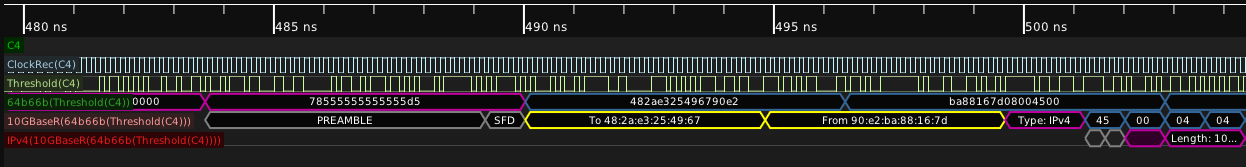
\includegraphics[width=16cm]{images/filters/64b66b.png}
%\caption{Example 64b/66b decode}
%\label{filter_64b66b}
%\end{figure}

\subsection{Inputs}

\begin{tabularx}{16cm}{llX}
\thickhline
\textbf{Signal name} & \textbf{Type} & \textbf{Description} \\
\thickhline
data & 1-bit digital & Serial 128b/130b data line \\
\thickhline
clk & 1-bit digital & DDR bit clock, typically generated by use of the \hyperref[filter:cdrpll]{Clock Recovery
(PLL)} filter on the input data.\\
\thickhline
\end{tabularx}

\subsection{Parameters}

This filter takes no parameters.

\subsection{Output Signal}

The 128B/130B filter outputs a time series of 128B/130B sample objects. These consist of a control/data flag and
a 128-bit data block.

\begin{tabularx}{16cm}{lllX}
\thickhline
\textbf{Type} & \textbf{Description} & \textbf{Color} & \textbf{Format} \\
\thickhline
Ordered set & Block with type 2'b10 & \cellcolor{control}\textcolor{white}{Control} & \%016x \\
\thickhline
Data & Block with type 2'b01 & \cellcolor{data}\textcolor{white}{Data} & \%016x \\
\thickhline
Error & Block with type 2'b00 or 2'b11 & \cellcolor{error}\textcolor{white}{Error} & \%016x \\
\thickhline
\end{tabularx}

%%%%%%%%%%%%%%%%%%%%%%%%%%%%%%%%%%%%%%%%%%%%%%%%%%%%%%%%%%%%%%%%%%%%%%%%%%%%%%%%%%%%%%%%%%%%%%%%%%%%%%%%%%%%%%%%%%%%%%%%
\pagebreak
\section{64b/66b}
\label{filter:64b66b}

Decodes the 64/66b line code used by \hyperref[filter:10gbaser]{10Gbase-R} and other serial protocols, as originally
specified in IEEE 802.3 clause 49.2.

64b/66b is a serial line code which divides transmitted data into 64-bit blocks and scrambles them with a LFSR, then
appends a 2-bit type field (which is not scrambled) to each block for synchronization. Block synchronization depends on
always having an edge in the type field so types 2'b00 and 2'b11 are disallowed.

Note that this filter only performs block alignment and descrambling. No decoding is applied to the 64-bit blocks, as
different upper-layer protocols assign different meaning to them. In 10Gbase-R, type 2'b01 denotes ``64 bits of upper
layer data" and type 2'b10 denotes ``8-bit type field and 56 bits of data whose meaning depends on the type", however
this is not universal.

\begin{figure}[h]
\centering
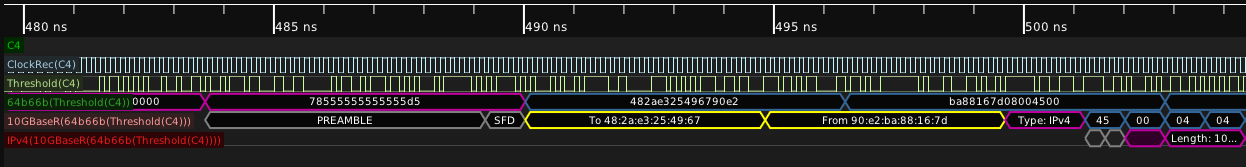
\includegraphics[width=16cm]{images/filters/64b66b.png}
\caption{Example 64b/66b decode}
\label{filter_64b66b}
\end{figure}

\subsection{Inputs}

\begin{tabularx}{16cm}{llX}
\thickhline
\textbf{Signal name} & \textbf{Type} & \textbf{Description} \\
\thickhline
data & 1-bit digital & Serial 64b/66b data line \\
\thickhline
clk & 1-bit digital & DDR bit clock, typically generated by use of the \hyperref[filter:cdrpll]{Clock Recovery
(PLL)} filter on the input data.\\
\thickhline
\end{tabularx}

\subsection{Parameters}

This filter takes no parameters.

\subsection{Output Signal}

The 64B/66B filter outputs a time series of 64B/66B sample objects. These consist of a control/data flag and
a 64-bit data block.

\begin{tabularx}{16cm}{lllX}
\thickhline
\textbf{Type} & \textbf{Description} & \textbf{Color} & \textbf{Format} \\
\thickhline
Control & Block with type 2'b10 & \cellcolor{control}\textcolor{white}{Control} & \%016x \\
\thickhline
Data & Block with type 2'b01 & \cellcolor{data}\textcolor{white}{Data} & \%016x \\
\thickhline
Error & Block with type 2'b00 or 2'b11 & \cellcolor{error}\textcolor{white}{Error} & \%016x \\
\thickhline
\end{tabularx}

%%%%%%%%%%%%%%%%%%%%%%%%%%%%%%%%%%%%%%%%%%%%%%%%%%%%%%%%%%%%%%%%%%%%%%%%%%%%%%%%%%%%%%%%%%%%%%%%%%%%%%%%%%%%%%%%%%%%%%%%
\pagebreak
\section{8B/10B (IBM)}
\label{filter:8b10b}

Decodes the standard 8b/10b line code used by SGMII, \hyperref[filter:1000basex]{1000base-X}, DisplayPort, JESD204,
\hyperref[filter:pcie2_logical]{PCIe gen 1/2}, SATA, USB 3.0, and many other common serial protocols.

8b/10b is a dictionary based code which converts each byte of message data to a ten-bit code. In order to maintain DC
balance and limit run length to a maximum of five identical bits in a row, all legal codes have one of:
\begin{itemize}
\item One legal coding, with exactly five zero bits
\item Two legal codings, one with four zero bits and one with six
\end{itemize}

The transmitter maintains a ``running disparity" counter and chooses the appropriate coding for each symbol to ensure
DC balance. There are twelve legal codes which are not needed for encoding data values; these are used to encode
frame boundaries, idle/alignment sequences, and other control information.

\begin{figure}[h]
\centering
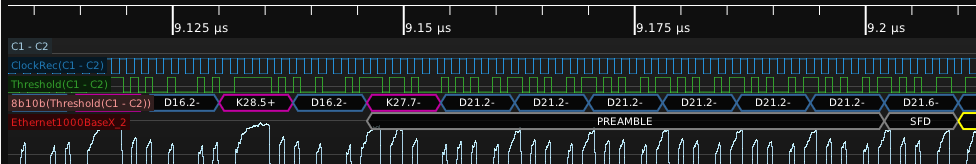
\includegraphics[width=16cm]{images/filters/8b10b.png}
\caption{Example 8b/10b decode}
\label{filter_8b10b}
\end{figure}

\subsection{Inputs}

\begin{tabularx}{16cm}{llX}
\thickhline
\textbf{Signal name} & \textbf{Type} & \textbf{Description} \\
\thickhline
data & 1-bit digital & Serial 8b/10b data line \\
\thickhline
clk & 1-bit digital & DDR bit clock, typically generated by use of the \hyperref[filter:cdrpll]{Clock Recovery
(PLL)} filter on the input data.\\
\thickhline
\end{tabularx}

\subsection{Parameters}

\begin{tabularx}{16cm}{llX}
\thickhline
\textbf{Parameter name} & \textbf{Type} & \textbf{Description} \\
\thickhline
Display Format & Enum &
	\textbf{Dotted (K28.5 D21.5)}: displays the 3b4b and 5b6b code blocks separately, with K or D prefix. \newline
	\textbf{Hex (K.bc b5)}: displays data as hex byte values and control codes with a K prefix. \\
\thickhline
\end{tabularx}

\subsection{Output Signal}

The 8B/10B filter outputs a time series of 8B/10B sample objects. These consist of a control/data flag and a byte of
data.

\begin{tabularx}{16cm}{lllX}
\thickhline
\textbf{Type} & \textbf{Description} & \textbf{Color} & \textbf{Format} \\
\thickhline
Control & Control codes & \cellcolor{control}\textcolor{white}{Control} & K\%d.\%d+ \\
\thickhline
Data & Upper layer protocol data & \cellcolor{data}\textcolor{white}{Data} & D\%d.\%d+ \\
\thickhline
Error & Malformed data & \cellcolor{error}\textcolor{white}{Error} & ERROR \\
\thickhline
\end{tabularx}

%%%%%%%%%%%%%%%%%%%%%%%%%%%%%%%%%%%%%%%%%%%%%%%%%%%%%%%%%%%%%%%%%%%%%%%%%%%%%%%%%%%%%%%%%%%%%%%%%%%%%%%%%%%%%%%%%%%%%%%%
\pagebreak
\section{8B/10B (TMDS)}
\label{filter:tmds}

Decodes the 8-to-10 Transition Minimized Differential Signalling line code used in \hyperref[filter:dvi]{DVI} and
\hyperref[filter:hdmi]{HDMI}.

Like the \hyperref[filter:8b10b]{8B/10B (IBM)} line code, TMDS is an 8-to-10 bit serial line code. TMDS, however, is
designed to \emph{minimize} the number of toggles in the data stream for EMC reasons, rendering it difficult to
synchronize a CDR PLL to. As a result, HDMI and DVI provide a reference clock at the pixel clock rate (1/10 the serial
data bit rate) along with the data stream to provide synchronization.

\begin{figure}[h]
\centering
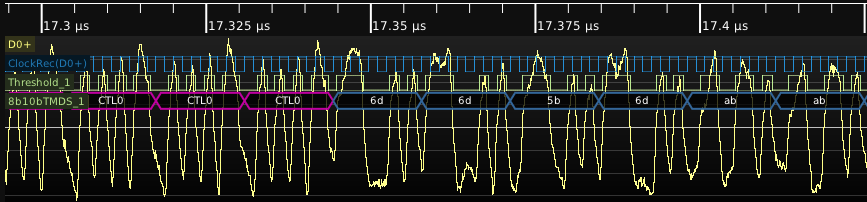
\includegraphics[width=16cm]{images/filters/tmds.png}
\caption{Example TMDS decode}
\label{filter_tmds}
\end{figure}

\subsection{Inputs}

\begin{tabularx}{16cm}{llX}
\thickhline
\textbf{Signal name} & \textbf{Type} & \textbf{Description} \\
\thickhline
data & 1-bit digital & Serial TMDS data line \\
\thickhline
clk & 1-bit digital & DDR \emph{bit} clock, typically generated by use of the \hyperref[filter:cdrpll]{Clock Recovery
(PLL)} filter on the input data. Note that this is 5x the rate of the pixel clock signal. \\
\thickhline
\end{tabularx}

\subsection{Parameters}

\begin{tabularx}{16cm}{llX}
\thickhline
\textbf{Parameter name} & \textbf{Type} & \textbf{Description} \\
\thickhline
Lane Number & Integer & Lane number within the link (0-3)\\
\thickhline
\end{tabularx}

\subsection{Output Signal}

The TMDS filter outputs a time series of TMDS sample objects. These consist of a type field and a byte of data.

The output of the TMDS decode is commonly fed to the \hyperref[filter:dvi]{DVI} or \hyperref[filter:hdmi]{HDMI}
protocol decoders.

\begin{tabularx}{16cm}{lllX}
\thickhline
\textbf{Type} & \textbf{Description} & \textbf{Color} & \textbf{Format} \\
\thickhline
Control & Control codes (H/V sync) & \cellcolor{control}\textcolor{white}{Control} & CTL\%d \\
\thickhline
Data & Pixel/island data & \cellcolor{data}\textcolor{white}{Data} & \%02x \\
\thickhline
Error & Malformed data & \cellcolor{error}\textcolor{white}{Error} & ERROR \\
\thickhline
Guard band & HDMI data/video guard band & \cellcolor{preamble}\textcolor{white}{Preamble} & GB \\
\thickhline
\end{tabularx}

%%%%%%%%%%%%%%%%%%%%%%%%%%%%%%%%%%%%%%%%%%%%%%%%%%%%%%%%%%%%%%%%%%%%%%%%%%%%%%%%%%%%%%%%%%%%%%%%%%%%%%%%%%%%%%%%%%%%%%%%
\pagebreak
\section{AC Couple}
\label{filter:accouple}

Automatically removes a DC offset from an analog waveform by subtracting the average of all samples from each sample.

This filter should only be used in postprocessing already acquired data, or other situations in which AC coupling in
the hardware (via an AC coupled probe, or coaxial DC block) is not possible.

\begin{figure}[h]
\centering
\includegraphics[width=16cm]{images/filters/ac-couple.png}
\caption{Example AC coupling}
\end{figure}

\subsection{Inputs}

\begin{tabularx}{16cm}{llX}
\thickhline
\textbf{Signal name} & \textbf{Type} & \textbf{Description} \\
\thickhline
din & Analog & Input waveform \\
\thickhline
\end{tabularx}

\subsection{Parameters}

This filter takes no parameters.

\subsection{Output Signal}

This filter outputs an analog waveform with identical sample rate to the input, vertically shifted to center the signal
at zero volts.

%%%%%%%%%%%%%%%%%%%%%%%%%%%%%%%%%%%%%%%%%%%%%%%%%%%%%%%%%%%%%%%%%%%%%%%%%%%%%%%%%%%%%%%%%%%%%%%%%%%%%%%%%%%%%%%%%%%%%%%%
\pagebreak
\section{AC RMS}
\label{filter:accouple}

Measures the Root Mean Square value of the waveform after removing any DC offset. This measurement can be made averaged
across the entire waveform, or on each cycle in the waveform.

\begin{figure}[h]
\centering
\includegraphics[width=16cm]{images/filters/ac-rms.png}
\caption{Example of an AC RMS Measurement of a Sinewave with 1V peak voltage}
\end{figure}

\subsection{Inputs}

\begin{tabularx}{16cm}{llX}
\thickhline
\textbf{Signal name} & \textbf{Type} & \textbf{Description} \\
\thickhline
din & Analog & Input waveform \\
\thickhline
\end{tabularx}

\subsection{Parameters}

\begin{tabularx}{16cm}{llX}
\thickhline
\textbf{Parameter name} & \textbf{Type} & \textbf{Description} \\
\thickhline
Measurement Type & Enum &
	\textbf{Average}: Measure the average AC RMS value\newline
	\textbf{Per Cycle}: Measure the per cycle AC RMS value\\
\thickhline
\end{tabularx}

\subsection{Output Signal}

This filter produces an output waveform only for the per cycle measurement type. This displays the AC RMS value of every cycle.

%%%%%%%%%%%%%%%%%%%%%%%%%%%%%%%%%%%%%%%%%%%%%%%%%%%%%%%%%%%%%%%%%%%%%%%%%%%%%%%%%%%%%%%%%%%%%%%%%%%%%%%%%%%%%%%%%%%%%%%%
\pagebreak
\section{Add}
\label{filter:add}

This filter adds two inputs. Either input may be a vector (waveform) or scalar. If both inputs are vectors, they must
have the same timebase.

%%%%%%%%%%%%%%%%%%%%%%%%%%%%%%%%%%%%%%%%%%%%%%%%%%%%%%%%%%%%%%%%%%%%%%%%%%%%%%%%%%%%%%%%%%%%%%%%%%%%%%%%%%%%%%%%%%%%%%%%
\pagebreak
\section{Area Under Curve}
\label{filter:AreaUnderCurve}

Measures the area under the curve by integrating the data points. By default, area measured above ground is considered
as positive and area measured below the ground is considered negative. The negative area can also be considered as positive
by changing a filter parameter. The measurement can be performed on the full record or on each cycle.

\begin{figure}[h]
\centering
\includegraphics[width=16cm]{images/filters/true-area.png}
\caption{Example of true area under the curve measurement (Integral)}
\end{figure}

\begin{figure}[h]
\centering
\includegraphics[width=16cm]{images/filters/absolute-area.png}
\caption{Example of absolute area under the curve measurement}
\end{figure}

\pagebreak

\begin{figure}[h]
\centering
\includegraphics[width=16cm]{images/filters/per-cycle-absolute-area.png}
\caption{Example of per-cycle absolute area under the curve measurement}
\end{figure}

\subsection{Inputs}

\begin{tabularx}{16cm}{llX}
\thickhline
\textbf{Signal name} & \textbf{Type} & \textbf{Description} \\
\thickhline
din & Analog & Input waveform \\
\thickhline
\end{tabularx}

\subsection{Parameters}

\begin{tabularx}{16cm}{llX}
\thickhline
\textbf{Parameter name} & \textbf{Type} & \textbf{Description} \\
\thickhline
Measurement Type & Enum &
	\textbf{Full Record}: Measure the area of entire waveform \newline
	\textbf{Per Cycle}: Measure the area of each cycle in the waveform\\
\thickhline
Area Type & Enum &
	\textbf{True Area}: Consider area below ground as negative\newline
	\textbf{Absolute Area}: Consider area below ground as positive\\
\thickhline
\end{tabularx}

\subsection{Output Signal}

For full record measurement, this filter outputs a waveform indicating total area measured till the time on the waveform.
For per cycle measurement, this filter outputs waveform representing area of each cycle.

%%%%%%%%%%%%%%%%%%%%%%%%%%%%%%%%%%%%%%%%%%%%%%%%%%%%%%%%%%%%%%%%%%%%%%%%%%%%%%%%%%%%%%%%%%%%%%%%%%%%%%%%%%%%%%%%%%%%%%%%
\pagebreak
\section{ADL5205}
\label{filter:adl5205}

Decodes SPI data traffic to one half of an ADL5205 variable gain amplifier.

TODO: Screenshot

\subsection{Inputs}

\begin{tabularx}{16cm}{llX}
\thickhline
\textbf{Signal name} & \textbf{Type} & \textbf{Description} \\
\thickhline
spi & SPI bus & The SPI data bus \\
\thickhline
\end{tabularx}

\subsection{Parameters}

This filter takes no parameters.

\subsection{Output Signal}

This filter outputs one ADL5205 sample object for each write transaction, formatted as ``write: FA=2 dB, gain=8 dB".

%%%%%%%%%%%%%%%%%%%%%%%%%%%%%%%%%%%%%%%%%%%%%%%%%%%%%%%%%%%%%%%%%%%%%%%%%%%%%%%%%%%%%%%%%%%%%%%%%%%%%%%%%%%%%%%%%%%%%%%%
\pagebreak
\section{Autocorrelation}
\label{filter:autocorrelation}

This filter calculates the autocorrelation of an analog waveform. Autocorrelation is a measure of self-similarity
calculated by multiplying the signal with a time-shifted copy of itself. In Fig. \ref{filter_accouple}, strong peaks
can be seen at multiples of the 8b/10b symbol rate.

For best performance, it is crucial to keep the maximum offset as low as possible, since filter run time grows linearly
with offset range.

\begin{figure}[h]
\centering
\includegraphics[width=16cm]{images/filters/autocorrelation.png}
\caption{Example of autocorrelation on a serial data stream}
\label{filter_accouple}
\end{figure}

\subsection{Inputs}

\begin{tabularx}{16cm}{llX}
\thickhline
\textbf{Signal name} & \textbf{Type} & \textbf{Description} \\
\thickhline
din & Analog & Input waveform \\
\thickhline
\end{tabularx}

\subsection{Parameters}

\begin{tabularx}{16cm}{llX}
\thickhline
\textbf{Parameter name} & \textbf{Type} & \textbf{Description} \\
\thickhline
Max offset & Integer & Maximum shift (in samples)\\
\thickhline
\end{tabularx}

\subsection{Output Signal}

This filter outputs an analog waveform with the same timebase as the input, one sample for each correlation offset.

%%%%%%%%%%%%%%%%%%%%%%%%%%%%%%%%%%%%%%%%%%%%%%%%%%%%%%%%%%%%%%%%%%%%%%%%%%%%%%%%%%%%%%%%%%%%%%%%%%%%%%%%%%%%%%%%%%%%%%%%
\pagebreak
\section{Base}
\label{filter:base}

Calculates the base (logical zero level) of each cycle in a digital waveform.

It is most commonly used as an input to statistics, to view the average base of the entire waveform. At times, however,
it may be useful to view the base waveform. For example, in Fig. \ref{filter_base}, the vertical eye closure caused by
channel ISI is readily apparent.

\begin{figure}[h]
\centering
\includegraphics[width=16cm]{images/filters/base.png}
\caption{Example of base measurement on a serial data stream}
\label{filter_base}
\end{figure}

\subsection{Inputs}

\begin{tabularx}{16cm}{llX}
\thickhline
\textbf{Signal name} & \textbf{Type} & \textbf{Description} \\
\thickhline
din & Analog & Input waveform \\
\thickhline
\end{tabularx}

\subsection{Parameters}

This filter takes no parameters.

\subsection{Output Signal}

This filter outputs an analog waveform with one sample for each group of logical zeroes in the input signal, containing
the average value of the zero level for the middle 50\% of the low period.

%%%%%%%%%%%%%%%%%%%%%%%%%%%%%%%%%%%%%%%%%%%%%%%%%%%%%%%%%%%%%%%%%%%%%%%%%%%%%%%%%%%%%%%%%%%%%%%%%%%%%%%%%%%%%%%%%%%%%%%%
\pagebreak
\section{BIN Import}

Loads an Agilent / Keysight / Rigol binary waveform file.

%%%%%%%%%%%%%%%%%%%%%%%%%%%%%%%%%%%%%%%%%%%%%%%%%%%%%%%%%%%%%%%%%%%%%%%%%%%%%%%%%%%%%%%%%%%%%%%%%%%%%%%%%%%%%%%%%%%%%%%%
\pagebreak
\section{Burst Width}

Measures the burst width of each burst in a waveform. A Burst is a sequence of adjacent crossings of the mid level reference
of the waveform. Burst width is the duration of this sequence. Bursts are separated by a user-defined idle time that can be
provided as a parameter to this filter. The measurement is made on each burst in the waveform.

\begin{figure}[h]
	\centering
	\includegraphics[width=16cm]{images/filters/burst-width.png}
	\caption{Example of burst width measurement}
	\label{filter_burstwidth}
	\end{figure}

\subsection{Inputs}

\begin{tabularx}{16cm}{llX}
\thickhline
\textbf{Signal name} & \textbf{Type} & \textbf{Description} \\
\thickhline
din & Analog & Input waveform \\
\thickhline
\end{tabularx}

\subsection{Parameters}

\begin{tabularx}{16cm}{llX}
\thickhline
\textbf{Parameter name} & \textbf{Type} & \textbf{Description} \\
\thickhline
Idle Time & Integer & Minimum idle time with no toggles, before declaring start of a new burst\\
\thickhline
\end{tabularx}

\subsection{Output Signal}

This filter outputs an analog waveform with one sample for each burst in the input signal.

%%%%%%%%%%%%%%%%%%%%%%%%%%%%%%%%%%%%%%%%%%%%%%%%%%%%%%%%%%%%%%%%%%%%%%%%%%%%%%%%%%%%%%%%%%%%%%%%%%%%%%%%%%%%%%%%%%%%%%%%
\pagebreak
\section{CAN}
\label{filter:can}

Decodes the Control Area Network (CAN) bus, commonly used in vehicle control systems. Both standard (11 bit) and
extended (29 bit) IDs are supported.

CAN-FD frames are detected and flagged as such, but the current decode cannot parse them fully. Full support is planned
(\issue{scopehal}{334}).

\begin{figure}[h]
\centering
\includegraphics[width=16cm]{images/filters/can.png}
\caption{Example of CAN bus protocol decode}
\label{filter_can}
\end{figure}

\subsection{Inputs}

\begin{tabularx}{16cm}{llX}
\thickhline
\textbf{Signal name} & \textbf{Type} & \textbf{Description} \\
\thickhline
CANH & Digital & Thresholded CANH (or CANH-CANL) signal \\
\thickhline
\end{tabularx}

\subsection{Parameters}

\begin{tabularx}{16cm}{llX}
\thickhline
\textbf{Parameter name} & \textbf{Type} & \textbf{Description} \\
\thickhline
Bit Rate & Integer & Bit rate of the bus (most commonly 250 or 500 Kbps)\\
\thickhline
\end{tabularx}

\subsection{Output Signal}

The CAN bus decode outputs a time series of CAN sample objects. These consist of a type field and a byte of data.

\begin{tabularx}{16cm}{lllX}
\thickhline
\textbf{Type} & \textbf{Description} & \textbf{Color} & \textbf{Format} \\
\thickhline
Control & Start of frame & \cellcolor{preamble}\textcolor{white}{Preamble} & SOF \\
\thickhline
ID & CAN ID & \cellcolor{address}\textcolor{black}{Address} & ID \%x \\
\thickhline
RTR & Remote Transmission Request & \cellcolor{control}\textcolor{white}{Control} & DATA | REQ \\
\thickhline
FD mode & CAN-FD mode & \cellcolor{control}\textcolor{white}{Control} & FD | STD\\
\thickhline
R0 & Reserved bits & \cellcolor{preamble}\textcolor{white}{Preamble} & RSVD \\
\thickhline
DLC & Data Length Code & \cellcolor{control}\textcolor{white}{Control} & Len 3 \\
\thickhline
Data & Payload data & \cellcolor{data}\textcolor{white}{Data} & \%02x \\
\thickhline
Valid CRC & Good checksum & \cellcolor{checksumok}\textcolor{black}{Checksum OK} & CRC: \%04x \\
\thickhline
Invalid CRC & Bad checksum & \cellcolor{checksumbad}\textcolor{white}{Checksum Bad} & CRC: \%04x \\
\thickhline
CRC delimiter & Bus turnaround & \cellcolor{preamble}\textcolor{white}{Preamble} & CRC DELIM \\
\thickhline
ACK & Acknowledgement & \cellcolor{checksumok}\textcolor{black}{Checksum OK} & ACK \\
\thickhline
NAK & Missing acknowledgement & \cellcolor{checksumbad}\textcolor{white}{Checksum Bad} & NAK \\
\thickhline
ACK delimiter & Bus turnaround & \cellcolor{preamble}\textcolor{white}{Preamble} & ACK DELIM \\
\thickhline
EOF & End of frame & \cellcolor{preamble}\textcolor{white}{Preamble} & EOF \\

\thickhline
\end{tabularx}

%%%%%%%%%%%%%%%%%%%%%%%%%%%%%%%%%%%%%%%%%%%%%%%%%%%%%%%%%%%%%%%%%%%%%%%%%%%%%%%%%%%%%%%%%%%%%%%%%%%%%%%%%%%%%%%%%%%%%%%%
\pagebreak
\section{Channel Emulation}
\label{filter:channelemu}

This filter models the effects of applying an arbitrary channel, described via a single path of a set of S-parameters,
to a waveform. Fig. \ref{filter_channelemu} shows the result of passing a 1.25 Gbps serial data pattern through S21 of
a 10x oscilloscope probe with approximately 500 MHz bandwidth. The ISI, attenuation, and phase shift introduced by the
channel can all be seen.

\begin{figure}[h]
\centering
\includegraphics[width=16cm]{images/filters/channel-emulation.png}
\caption{Example of channel emulation on a serial data stream}
\label{filter_channelemu}
\end{figure}

The channel model works in the frequency domain. An FFT is performed on the input, then each complex point is scaled by
the interpolated magnitude and rotated by the phase, then an inverse FFT is used to transform the signal back into the
time domain.

The group delay of the channel is then estimated and samples are discarded from the beginning of the waveform to
prevent causality violations. For example, when performing channel emulation using a network with a 1ns group delay,
the output waveform will begin 1ns after the input (since the channel output before this depends on input samples
before the start of the waveform). Note that the automatic group delay estimation uses points from roughly the center
of the S-parameter dataset in the current implementation; channels which do not have a significant passband around this
frequency will give incorrect group delay estimates. The ``Group Delay Truncation Mode" parameter can be set to manual
in this case, selecting the ``Group Delay Truncation" parameter instead of the automatically estimated value.

By choosing appropriate stimulus waveforms and S-parameter paths, many different kinds of analysis can be performed.
For example, given a 4-port network describing two transmission lines (with ports 1 and 3 as input, and 2 and 4 as
output):
\begin{itemize}
\item Applying $S_{11}$ to a step or impulse waveform gives TDR response of the port 1-2 channel.
\item Applying $S_{21}$ to an impulse waveform gives impulse response of the port 1-2 channel
\item Applying $S_{21}$ to a serial data stream gives the port 1-2 signal as it would be seen by a receiver
\item Applying $S_{31}$ to a serial data stream gives the NEXT between the port 1-2 and 3-4 channels
\item Applying $S_{41}$ to a serial data stream gives the FEXT between the port 1-2 and 3-4 channels
\end{itemize}

Note that only the single S-parameter path provided is considered, and reflections elsewhere in the system are not
modeled. As a result, multiple applications of this filter to emulate a large circuit piecewise (for example, a
cable followed by a fixture) may give inaccurate results since reflections between the two networks are not considered.
In this situation, it is preferable to use a circuit simulator to calculate combined S-parameters of the entire circuit
and then perform the channel emulation once.

\subsection{Inputs}

\begin{tabularx}{16cm}{llX}
\thickhline
\textbf{Signal name} & \textbf{Type} & \textbf{Description} \\
\thickhline
signal & Analog & Input waveform \\
\thinhline
mag & Analog & S-parameter magnitude channel \\
\thinhline
ang & Analog & S-parameter angle channel \\
\thickhline
\end{tabularx}

\subsection{Parameters}

\begin{tabularx}{16cm}{llX}
\thickhline
\textbf{Parameter name} & \textbf{Type} & \textbf{Description} \\
\thickhline
Max Gain & Float & Maximum gain to apply\\
\thinhline
Group Delay Truncation & Int & Group delay override for manual mode\\
\thinhline
Group Delay Truncation Mode & Enum & Specifies manual or automatically estimated group delay\\
\thickhline
\end{tabularx}

\subsection{Output Signal}

This filter outputs an analog waveform with the same timebase as the input, with the emulated channel applied.

%%%%%%%%%%%%%%%%%%%%%%%%%%%%%%%%%%%%%%%%%%%%%%%%%%%%%%%%%%%%%%%%%%%%%%%%%%%%%%%%%%%%%%%%%%%%%%%%%%%%%%%%%%%%%%%%%%%%%%%%
\pagebreak
\section{Clip}
\label{filter:clip}

This filter limits the maximum or minimum value of a waveform to a given value. It can be configured
to clip ``above" in which case it imposes an upper limit or ``below" in which case it imposes a lower
limit.

\subsection{Inputs}

\begin{tabularx}{16cm}{llX}
\thickhline
\textbf{Signal name} & \textbf{Type} & \textbf{Description} \\
\thickhline
din & Analog & Input waveform \\
\thickhline
\end{tabularx}

\subsection{Parameters}

\begin{tabularx}{16cm}{llX}
\thickhline
\textbf{Parameter name} & \textbf{Type} & \textbf{Description} \\
\thickhline
Behavior & Enum & Select between clipping values above or below selected value\\
\thinhline
Level & Float & Maximum/minimum signal level\\
\thickhline
\end{tabularx}

\subsection{Output Signal}

This filter outputs an analog waveform with the same timebase as the input, clipped as specified by the parameters.

%%%%%%%%%%%%%%%%%%%%%%%%%%%%%%%%%%%%%%%%%%%%%%%%%%%%%%%%%%%%%%%%%%%%%%%%%%%%%%%%%%%%%%%%%%%%%%%%%%%%%%%%%%%%%%%%%%%%%%%%
\pagebreak
\section{Clock Recovery (D-PHY HS Mode)}

Extracts a double-rate clock from a MIPI D-PHY clock+data stream, which is gated to only toggle when the data input
is in HS mode. This can be used for generating eye patterns of the HS-mode data.

%%%%%%%%%%%%%%%%%%%%%%%%%%%%%%%%%%%%%%%%%%%%%%%%%%%%%%%%%%%%%%%%%%%%%%%%%%%%%%%%%%%%%%%%%%%%%%%%%%%%%%%%%%%%%%%%%%%%%%%%
\pagebreak
\section{Clock Recovery (PLL)}
\label{filter:cdrpll}

This filter uses a PLL to recover a clock from a serial data stream. The recovered clock is double-rate and
phased 90\textdegree with respect to the data, such that the data can be sampled directly by both edges of the PLL
output clock.

When the optional clock gating input is low, the output does not toggle and any edges in the input signal are ignored.
As soon as the gate goes high, the PLL will phase shift the internal NCO to align with the next transition in the input
signal and then begin running closed-loop.

NOTE: The current edge detector uses a single threshold suitable for NRZ inputs. When using a multi-level modulation
such as PAM-4 or MLT-3, set the threshold to the highest or lowest crossing level. This will work fine for MLT-3 but
introduces some data-dependent jitter in PAM signals (since the slew rate for an 00-11 transition is different than
that for a 10-11 transition). The resulting recovered clock should still be adequate for protocol decoding, however a
better edge detector will need to be implemented in order to do adequate jitter measurements on PAM waveforms. An edge
detector suitable for PAM is planned (\issue{scopehal}{77}).

The current implementation of this filter uses a simple bang-bang control loop which is fast and provides reasonable
jitter transfer performance (passing high frequency jitter but rejecting spread spectrum modulation), but does not
precisely match the jitter transfer characteristics of any particular serial data standard. In the future, several
standard PLL responses including the Fibre Channel golden PLL (\issue{scopehal}{163}) will be supported as options.

\begin{figure}[h]
\centering
\includegraphics[width=16cm]{images/filters/cdrpll.png}
\caption{Example of CDR PLL on a serial data stream}
\label{filter_cdrpll}
\end{figure}

\subsection{Inputs}

\begin{tabularx}{16cm}{llX}
\thickhline
\textbf{Signal name} & \textbf{Type} & \textbf{Description} \\
\thickhline
IN & Analog & Input waveform \\
\thinhline
Gate & Digital & Clock enable signal, or NULL to disable gating\\
\thickhline
\end{tabularx}

\subsection{Parameters}

\begin{tabularx}{16cm}{llX}
\thickhline
\textbf{Parameter name} & \textbf{Type} & \textbf{Description} \\
\thickhline
Symbol rate & Float & Symbol rate, in Hz\\
\thinhline
Threshold & Float & Decision threshold for the edge detector, in volts\\
\thickhline
\end{tabularx}

\subsection{Output Signal}

This filter outputs an digital waveform with one sample per transition of the recovered clock.

%%%%%%%%%%%%%%%%%%%%%%%%%%%%%%%%%%%%%%%%%%%%%%%%%%%%%%%%%%%%%%%%%%%%%%%%%%%%%%%%%%%%%%%%%%%%%%%%%%%%%%%%%%%%%%%%%%%%%%%%
\pagebreak
\section{Clock Recovery (UART)}

Simple DLL suitable for displaying eye patterns of RS232 and similar protocols.

%%%%%%%%%%%%%%%%%%%%%%%%%%%%%%%%%%%%%%%%%%%%%%%%%%%%%%%%%%%%%%%%%%%%%%%%%%%%%%%%%%%%%%%%%%%%%%%%%%%%%%%%%%%%%%%%%%%%%%%%
\pagebreak
\section{Complex Import}

Loads waveform data from a raw binary file containing I/Q samples in one of several formats. Regardless of sample
format, the samples must be in I-Q-I-Q order.

Supported formats (native endianness, no byte swapping is performed):
\begin{itemize}
\item Signed int8
\item Unsigned int8
\item Signed int16
\item Float32
\item Float64
\end{itemize}

\subsection{Inputs}

This filter takes no inputs.

\subsection{Parameters}

\begin{tabularx}{16cm}{llX}
\thickhline
\textbf{Parameter name} & \textbf{Type} & \textbf{Description} \\
\thickhline
Complex File & String & Path to the input file\\
\thinhline
File Format & Enum & Data type of the samples\\
\thinhline
Sample Rate & Int & Sampling frequency\\
\thickhline
\end{tabularx}

\subsection{Output Signal}

This filter outputs two streams named ``I" and ``Q" containing the I/Q waveform data.

%%%%%%%%%%%%%%%%%%%%%%%%%%%%%%%%%%%%%%%%%%%%%%%%%%%%%%%%%%%%%%%%%%%%%%%%%%%%%%%%%%%%%%%%%%%%%%%%%%%%%%%%%%%%%%%%%%%%%%%%
\pagebreak
\section{Constant}
\label{filter:constant}

This filter outputs a scalar with a constant value, which may be used as input to other filter graph blocks.

%%%%%%%%%%%%%%%%%%%%%%%%%%%%%%%%%%%%%%%%%%%%%%%%%%%%%%%%%%%%%%%%%%%%%%%%%%%%%%%%%%%%%%%%%%%%%%%%%%%%%%%%%%%%%%%%%%%%%%%%
\pagebreak
\section{CSV Export}

Saves waveform data to a comma-separated-value file.

%%%%%%%%%%%%%%%%%%%%%%%%%%%%%%%%%%%%%%%%%%%%%%%%%%%%%%%%%%%%%%%%%%%%%%%%%%%%%%%%%%%%%%%%%%%%%%%%%%%%%%%%%%%%%%%%%%%%%%%%
\pagebreak
\section{CSV Import}

Loads waveform data from a comma-separated-value file.


%%%%%%%%%%%%%%%%%%%%%%%%%%%%%%%%%%%%%%%%%%%%%%%%%%%%%%%%%%%%%%%%%%%%%%%%%%%%%%%%%%%%%%%%%%%%%%%%%%%%%%%%%%%%%%%%%%%%%%%%
\pagebreak
\section{Current Shunt}

Converts a voltage waveform acquired across a known resistance into a current waveform.

%%%%%%%%%%%%%%%%%%%%%%%%%%%%%%%%%%%%%%%%%%%%%%%%%%%%%%%%%%%%%%%%%%%%%%%%%%%%%%%%%%%%%%%%%%%%%%%%%%%%%%%%%%%%%%%%%%%%%%%%
\pagebreak
\section{DDJ}
\label{filter:ddj}

Calculates the peak-to-peak data-dependent jitter for a serial data stream.

This filter uses the non-repeating-pattern method, which allows DDJ to be computed for arbitrary waveforms rather than
requiring a short, repeating PRBS. In this method, per-UI jitter (TIE) measurements are split across $2^n$ histogram
bins, one for each possible combination of the preceding $n$ bits. The jitter samples for each bin are then averaged to
remove the effects of other jitter, leaving only the DDJ.  The final DDJ value is reported as the difference between
the minimum and maximum histogram bins.

The current implementation uses a fixed window size of $n=8$ UI. If the channel has significant memory effects or
reflections with delays of more than 8 UI, DDJ maybe underestimated.

The current implementation only supports NRZ signals and cannot measure DDJ for MLT3 or PAM waveforms.

\subsection{Inputs}

\begin{tabularx}{16cm}{llX}
\thickhline
\textbf{Signal name} & \textbf{Type} & \textbf{Description} \\
\thickhline
TIE & Analog & TIE waveform computed by the \hyperref[filter:tie]{TIE} filter\\
\thinhline
Threshold & Digital & Thresholded digital sample values\\
\thinhline
Clock & Digital & Double rate, center aligned sampling clock for threshold values\\
\thickhline
\end{tabularx}

\subsection{Parameters}

This filter takes no parameters.

\subsection{Output Signal}

This filter outputs an analog waveform with a single sample containing the computed DDJ value.

Additionally, the raw DDJ histogram is stored internally and may be accessed by other filters via the C++ API. There is
currently no way to display the histogram content.

%%%%%%%%%%%%%%%%%%%%%%%%%%%%%%%%%%%%%%%%%%%%%%%%%%%%%%%%%%%%%%%%%%%%%%%%%%%%%%%%%%%%%%%%%%%%%%%%%%%%%%%%%%%%%%%%%%%%%%%%
\pagebreak
\section{DDR1 Command Bus}

Decodes the command bus for first-generation DDR SDRAM.

%%%%%%%%%%%%%%%%%%%%%%%%%%%%%%%%%%%%%%%%%%%%%%%%%%%%%%%%%%%%%%%%%%%%%%%%%%%%%%%%%%%%%%%%%%%%%%%%%%%%%%%%%%%%%%%%%%%%%%%%
\pagebreak
\section{DDR3 Command Bus}

Decodes the command bus for third-generation DDR SDRAM.

%%%%%%%%%%%%%%%%%%%%%%%%%%%%%%%%%%%%%%%%%%%%%%%%%%%%%%%%%%%%%%%%%%%%%%%%%%%%%%%%%%%%%%%%%%%%%%%%%%%%%%%%%%%%%%%%%%%%%%%%
\pagebreak
\section{De-Embed}
\label{filter:deembed}

Applies the inverse of a channel (described by a single path in an S-parameter dataset, normally $S_{21}$) to a signal,
in order to calculate what the waveform would have looked like at the input to a cable, fixture, etc. given the signal
seen at the output.

The channel model works in the frequency domain. An FFT is performed on the input, then each complex point is scaled by
the interpolated magnitude and rotated by the phase, then an inverse FFT is used to transform the signal back into the
time domain.

The group delay of the channel is then estimated and samples are discarded from the end of the waveform to prevent
causality violations. For example, when performing a de-embed using a network with a 1ns group delay, the output
waveform will end 1ns before the input does (since the channel output after this depends on input samples after the end
of the stimulus waveform). Note that the automatic group delay estimation uses points from roughly the center of the
S-parameter dataset in the current implementation; channels which do not have a significant passband around this
frequency will give incorrect group delay estimates. The ``Group Delay Truncation Mode" parameter can be set to manual
in this case, selecting the ``Group Delay Truncation" parameter instead of the automatically estimated value.

Note that only the single S-parameter path provided is considered, and reflections elsewhere in the system are not
modeled. As a result, multiple applications of this filter to de-embed a large circuit piecewise (for example, a cable
followed by a probe) may give inaccurate results since reflections between the two networks are not considered. In this
situation, it is preferable to use a circuit simulator or the \hyperref[filter:sparamcascade]{S-Parameter Cascade}
filter to calculate combined S-parameters of the entire circuit and then perform a single de-embed.

The maximum gain the de-embed applies is capped (default 20 dB) in order to prevent amplifying noise outside the
passband of the network being de-embedded.

\subsection{Inputs}

\begin{tabularx}{16cm}{llX}
\thickhline
\textbf{Signal name} & \textbf{Type} & \textbf{Description} \\
\thickhline
signal & Analog & Input waveform \\
\thinhline
mag & Analog & S-parameter magnitude channel \\
\thinhline
ang & Analog & S-parameter angle channel \\
\thickhline
\end{tabularx}

\subsection{Parameters}

\begin{tabularx}{16cm}{llX}
\thickhline
\textbf{Parameter name} & \textbf{Type} & \textbf{Description} \\
\thickhline
Max Gain & Float & Maximum gain to apply\\
\thinhline
Group Delay Truncation & Int & Group delay override for manual mode\\
\thinhline
Group Delay Truncation Mode & Enum & Specifies manual or automatically estimated group delay\\
\thickhline
\end{tabularx}

\subsection{Output Signal}

This filter outputs an analog waveform with the same timebase as the input, with the emulated channel applied.

%%%%%%%%%%%%%%%%%%%%%%%%%%%%%%%%%%%%%%%%%%%%%%%%%%%%%%%%%%%%%%%%%%%%%%%%%%%%%%%%%%%%%%%%%%%%%%%%%%%%%%%%%%%%%%%%%%%%%%%%
\pagebreak
\section{Deskew}
\label{filter:deskew}

Moves an analog waveform earlier or later in time to compensate for trigger offsets, probe length mismatch, etc.
It is generally preferable to deskew using the skew adjustment on the channel during acquisition; this filter is
provided for correction in postprocessing.

\subsection{Inputs}

\begin{tabularx}{16cm}{llX}
\thickhline
\textbf{Signal name} & \textbf{Type} & \textbf{Description} \\
\thickhline
din & Analog & Input waveform \\
\thickhline
\end{tabularx}

\subsection{Parameters}

\begin{tabularx}{16cm}{llX}
\thickhline
\textbf{Parameter name} & \textbf{Type} & \textbf{Description} \\
\thickhline
Skew & Float & Time offset to shift the waveform\\
\thickhline
\end{tabularx}

\subsection{Output Signal}

This filter outputs an analog waveform with one sample for each sample in the input, phase shifted by the requested
offset.

%%%%%%%%%%%%%%%%%%%%%%%%%%%%%%%%%%%%%%%%%%%%%%%%%%%%%%%%%%%%%%%%%%%%%%%%%%%%%%%%%%%%%%%%%%%%%%%%%%%%%%%%%%%%%%%%%%%%%%%%
\pagebreak
\section{Digital to NRZ}
\label{filter:digitaltonrz}

Convert a digital signal (and associated clock) to an analog NRZ waveform. This filter uses a simplistic piecewise
linear rise/fall time model: the output stays at the logic low/high voltage until the input changes, then ramps at a
constant rate to then new value. For more accurate modeling of edge shape use the \hyperref[filter:ibisdriver]{IBIS
Driver} filter with the appropriate IBIS model for your DUT.

\subsection{Inputs}

\begin{tabularx}{16cm}{llX}
\thickhline
\textbf{Signal name} & \textbf{Type} & \textbf{Description} \\
\thickhline
data & Digital & Digital data to send\\
\thinhline
clk & Digital & Clock for data\\
\thickhline
\end{tabularx}

\subsection{Parameters}

\begin{tabularx}{16cm}{llX}
\thickhline
\textbf{Parameter name} & \textbf{Type} & \textbf{Description} \\
\thickhline
Level 0 & Float & Voltage to send when the input is a logic 0\\
\thinhline
Level 1 & Float & Voltage to send when the input is a logic 1\\
\thinhline
Sample Rate & Int & Sample rate for the generated waveform\\
\thinhline
Transition Time & Int & Rising and falling edge time\\
\thickhline
\end{tabularx}

\subsection{Output Signal}

This filter outputs an analog NRZ version of the provided digital input, sampled uniformly at the specified rate.

%%%%%%%%%%%%%%%%%%%%%%%%%%%%%%%%%%%%%%%%%%%%%%%%%%%%%%%%%%%%%%%%%%%%%%%%%%%%%%%%%%%%%%%%%%%%%%%%%%%%%%%%%%%%%%%%%%%%%%%%
\pagebreak
\section{Digital to PAM4}
\label{filter:digitaltopam4}

Convert a digital signal (and associated clock) to an analog PAM-4 waveform. This filter uses a simplistic piecewise
linear rise/fall time model: the output stays at the current symbol's voltage until the input changes, then ramps at a
constant rate to then new value. For more accurate modeling of edge shape use the \hyperref[filter:ibisdriver]{IBIS
Driver} filter with the appropriate IBIS model for your DUT.

The input data is a digital serial bit stream at twice the PAM4 symbol rate. Two consecutive input bits map to a single
PAM-4 output sample.

\subsection{Inputs}

\begin{tabularx}{16cm}{llX}
\thickhline
\textbf{Signal name} & \textbf{Type} & \textbf{Description} \\
\thickhline
data & Digital & Serial digital data to send\\
\thinhline
clk & Digital & Clock for data\\
\thickhline
\end{tabularx}

\subsection{Parameters}

\begin{tabularx}{16cm}{llX}
\thickhline
\textbf{Parameter name} & \textbf{Type} & \textbf{Description} \\
\thickhline
Level 00 & Float & Voltage to send when the input is a logic 0-0\\
\thinhline
Level 01 & Float & Voltage to send when the input is a logic 0-1\\
\thinhline
Level 10 & Float & Voltage to send when the input is a logic 1-0\\
\thinhline
Level 11 & Float & Voltage to send when the input is a logic 1-1\\
\thinhline
Sample Rate & Int & Sample rate for the generated waveform\\
\thinhline
Transition Time & Int & Rising and falling edge time\\
\thickhline
\end{tabularx}

\subsection{Output Signal}

This filter outputs an analog PAM-4 version of the provided digital input, sampled uniformly at the specified rate.

%%%%%%%%%%%%%%%%%%%%%%%%%%%%%%%%%%%%%%%%%%%%%%%%%%%%%%%%%%%%%%%%%%%%%%%%%%%%%%%%%%%%%%%%%%%%%%%%%%%%%%%%%%%%%%%%%%%%%%%%
\pagebreak
\section{DisplayPort - Aux Channel}

Decodes the Auxiliary Channel of DisplayPort

%%%%%%%%%%%%%%%%%%%%%%%%%%%%%%%%%%%%%%%%%%%%%%%%%%%%%%%%%%%%%%%%%%%%%%%%%%%%%%%%%%%%%%%%%%%%%%%%%%%%%%%%%%%%%%%%%%%%%%%%
\pagebreak
\section{Divide}

Divides one waveform by another.

%%%%%%%%%%%%%%%%%%%%%%%%%%%%%%%%%%%%%%%%%%%%%%%%%%%%%%%%%%%%%%%%%%%%%%%%%%%%%%%%%%%%%%%%%%%%%%%%%%%%%%%%%%%%%%%%%%%%%%%%
\pagebreak
\section{Downconvert}

Performs digital downconversion by mixing a directly sampled RF signal with a two-phase local oscillator, then outputs
the downconverted signal. No LO rejection filtering or decimation is performed.

%%%%%%%%%%%%%%%%%%%%%%%%%%%%%%%%%%%%%%%%%%%%%%%%%%%%%%%%%%%%%%%%%%%%%%%%%%%%%%%%%%%%%%%%%%%%%%%%%%%%%%%%%%%%%%%%%%%%%%%%
\pagebreak
\section{Downsample}

Low-pass filters a signal to prevent aliasing, then decimates by an integer factor.

%%%%%%%%%%%%%%%%%%%%%%%%%%%%%%%%%%%%%%%%%%%%%%%%%%%%%%%%%%%%%%%%%%%%%%%%%%%%%%%%%%%%%%%%%%%%%%%%%%%%%%%%%%%%%%%%%%%%%%%%
\pagebreak
\section{DRAM Clocks}

Given a DRAM command bus and a DQS strobe, produce separate gated DQ clock streams for read and write bursts.

%%%%%%%%%%%%%%%%%%%%%%%%%%%%%%%%%%%%%%%%%%%%%%%%%%%%%%%%%%%%%%%%%%%%%%%%%%%%%%%%%%%%%%%%%%%%%%%%%%%%%%%%%%%%%%%%%%%%%%%%
\pagebreak
\section{DRAM Trcd}

Calculates $T_{rcd}$ (RAS-to-CAS delay) for each newly opened row in a DRAM command bus stream.

%%%%%%%%%%%%%%%%%%%%%%%%%%%%%%%%%%%%%%%%%%%%%%%%%%%%%%%%%%%%%%%%%%%%%%%%%%%%%%%%%%%%%%%%%%%%%%%%%%%%%%%%%%%%%%%%%%%%%%%%
\pagebreak
\section{DRAM Trfc}

Calculates $T_{rfc}$ (refresh-to-refresh delay) for each refresh operation in a DRAM command bus stream.

%%%%%%%%%%%%%%%%%%%%%%%%%%%%%%%%%%%%%%%%%%%%%%%%%%%%%%%%%%%%%%%%%%%%%%%%%%%%%%%%%%%%%%%%%%%%%%%%%%%%%%%%%%%%%%%%%%%%%%%%
\pagebreak
\section{Duty Cycle}

Calculates the duty cycle of a bimodal waveform. The duty cycle is defined as the percentage of time spent in the high
state divided by the period.

%%%%%%%%%%%%%%%%%%%%%%%%%%%%%%%%%%%%%%%%%%%%%%%%%%%%%%%%%%%%%%%%%%%%%%%%%%%%%%%%%%%%%%%%%%%%%%%%%%%%%%%%%%%%%%%%%%%%%%%%
\pagebreak
\section{DVI}
\label{filter:dvi}

Decodes Digital Visual Interface (DVI) video signals.

%%%%%%%%%%%%%%%%%%%%%%%%%%%%%%%%%%%%%%%%%%%%%%%%%%%%%%%%%%%%%%%%%%%%%%%%%%%%%%%%%%%%%%%%%%%%%%%%%%%%%%%%%%%%%%%%%%%%%%%%
\pagebreak
\section{Emphasis}

Adds pre/de emphasis to a signal.

%%%%%%%%%%%%%%%%%%%%%%%%%%%%%%%%%%%%%%%%%%%%%%%%%%%%%%%%%%%%%%%%%%%%%%%%%%%%%%%%%%%%%%%%%%%%%%%%%%%%%%%%%%%%%%%%%%%%%%%%
\pagebreak
\section{Emphasis Removal}

Removes pre/de emphasis from a signal.

%%%%%%%%%%%%%%%%%%%%%%%%%%%%%%%%%%%%%%%%%%%%%%%%%%%%%%%%%%%%%%%%%%%%%%%%%%%%%%%%%%%%%%%%%%%%%%%%%%%%%%%%%%%%%%%%%%%%%%%%
\pagebreak
\section{Enhanced Resolution}
\label{filter:eres}

Applies a FIR low-pass filter to a signal to increase the vertical resolution and reduce noise at the cost of reduced
bandwidth. This technique assumes a small amount of Gaussian noise is present in the input waveform, such that a signal
whose true value is midway between two ADC codes will randomly fluctuate between the two quantized values, with an
average equal to the true value.

Each half bit of resolution reduces the bandwidth by an additional factor of two beyond the Nyquist limit. For example,
a 1.5 bit resolution improvement reduces the bandwith to Fnyquist / 8. The filter properties dialog displays the
calculated -3 dB bandwidth based on the current input sample rate.

\subsection{Inputs}

\begin{tabularx}{16cm}{llX}
\thickhline
\textbf{Signal name} & \textbf{Type} & \textbf{Description} \\
\thickhline
in & Analog & Input signal\\
\thickhline
\end{tabularx}

\subsection{Parameters}

\begin{tabularx}{16cm}{llX}
\thickhline
\textbf{Parameter name} & \textbf{Type} & \textbf{Description} \\
\thickhline
Bits & Enum & Number of additional bits of resolution to add\\
\thickhline
\end{tabularx}

%%%%%%%%%%%%%%%%%%%%%%%%%%%%%%%%%%%%%%%%%%%%%%%%%%%%%%%%%%%%%%%%%%%%%%%%%%%%%%%%%%%%%%%%%%%%%%%%%%%%%%%%%%%%%%%%%%%%%%%%
\pagebreak
\section{Envelope}
\label{filter:envelope}

Finds the minimum and maximum of each sample in the input over time, and outputs them as separate streams.

%%%%%%%%%%%%%%%%%%%%%%%%%%%%%%%%%%%%%%%%%%%%%%%%%%%%%%%%%%%%%%%%%%%%%%%%%%%%%%%%%%%%%%%%%%%%%%%%%%%%%%%%%%%%%%%%%%%%%%%%
\pagebreak
\section{Ethernet - 10baseT}

Decodes the 10base-T Ethernet PCS/PMA as specified in IEEE 802.3-2018 clause 14.

%%%%%%%%%%%%%%%%%%%%%%%%%%%%%%%%%%%%%%%%%%%%%%%%%%%%%%%%%%%%%%%%%%%%%%%%%%%%%%%%%%%%%%%%%%%%%%%%%%%%%%%%%%%%%%%%%%%%%%%%
\pagebreak
\section{Ethernet - 100baseTX}

Decodes the 100base-TX Ethernet PMA/PCS as specified in IEEE 802.3-2018 clause 24 and 25, and the ANSI X3T12 FDDI PHY.

%%%%%%%%%%%%%%%%%%%%%%%%%%%%%%%%%%%%%%%%%%%%%%%%%%%%%%%%%%%%%%%%%%%%%%%%%%%%%%%%%%%%%%%%%%%%%%%%%%%%%%%%%%%%%%%%%%%%%%%%
\pagebreak
\section{Ethernet - 1000baseX}
\label{proto:1000basex}

Decodes the 1000base-X Ethernet PCS as specified in IEEE 802.3-2018 clause 36.

\begin{tabularx}{16cm}{llX}
\thickhline
\textbf{Signal name} & \textbf{Type} & \textbf{Description} \\
\thickhline
data & 8b/10b & Output of \hyperref[proto:8b10b]{8b/10b protocol decode}\\
\thickhline
\end{tabularx}

\subsection{Parameters}

This filter takes no parameters.

\subsection{Output Signal}

The 1000base-X filter outputs a series of Ethernet frame segment objects.

\begin{tabularx}{16cm}{lllX}
\thickhline
\textbf{Type} & \textbf{Description} & \textbf{Color} & \textbf{Format} \\
\thickhline
Preamble & Preamble & \cellcolor{preamble}\textcolor{white}{Preamble} & PREAMBLE \\
\thickhline
Preamble & Start of frame delimiter & \cellcolor{preamble}\textcolor{white}{Preamble} & SFD \\
\thickhline
Address & Src/dest MAC & \cellcolor{address}\textcolor{black}{Address} & From 02:00:11:22:33:44 \\
\thickhline
Control & Ethertype & \cellcolor{control}\textcolor{white}{Control} & Type: IPv4 \newline Type: 0xbeef \\
\thickhline
Control & VLAN tag & \cellcolor{control}\textcolor{white}{Control} & VLAN 10, PCP 0 \\
\thickhline
Data & Frame data & \cellcolor{data}\textcolor{white}{Data} & a5 \\
\thickhline
Checksum OK & Valid FCS & \cellcolor{checksumok}\textcolor{black}{Checksum OK} & CRC: 0xdeadbeef \\
\thickhline
Checksum Bad & Invalid FCS & \cellcolor{checksumbad}\textcolor{white}{Checksum Bad} & CRC: 0xbaadc0de \\
\thickhline
Error & Malformed data & \cellcolor{error}\textcolor{white}{Error} & ERROR \\
\thickhline
\end{tabularx}

TODO: Document protocol analyzer output

%%%%%%%%%%%%%%%%%%%%%%%%%%%%%%%%%%%%%%%%%%%%%%%%%%%%%%%%%%%%%%%%%%%%%%%%%%%%%%%%%%%%%%%%%%%%%%%%%%%%%%%%%%%%%%%%%%%%%%%%
\pagebreak
\section{Ethernet - GMII}

Decodes the Gigabit Media Independent Interface as specified in IEEE 802.3-2018 clause 35.

%%%%%%%%%%%%%%%%%%%%%%%%%%%%%%%%%%%%%%%%%%%%%%%%%%%%%%%%%%%%%%%%%%%%%%%%%%%%%%%%%%%%%%%%%%%%%%%%%%%%%%%%%%%%%%%%%%%%%%%%
\pagebreak
\section{Ethernet - QSGMII}

Converts a Quad SGMII data stream into four separate SGMII data streams which can be independently decoded.

%%%%%%%%%%%%%%%%%%%%%%%%%%%%%%%%%%%%%%%%%%%%%%%%%%%%%%%%%%%%%%%%%%%%%%%%%%%%%%%%%%%%%%%%%%%%%%%%%%%%%%%%%%%%%%%%%%%%%%%%
\pagebreak
\section{Ethernet - RGMII}

Decodes the Reduced Gigabit Media Independent Interface as specified in the RGMII 2.0 specification.

%%%%%%%%%%%%%%%%%%%%%%%%%%%%%%%%%%%%%%%%%%%%%%%%%%%%%%%%%%%%%%%%%%%%%%%%%%%%%%%%%%%%%%%%%%%%%%%%%%%%%%%%%%%%%%%%%%%%%%%%
\pagebreak
\section{Ethernet - RMII}

Decodes the Reduced Media Independent Interface as specified in the RMII specification.

%%%%%%%%%%%%%%%%%%%%%%%%%%%%%%%%%%%%%%%%%%%%%%%%%%%%%%%%%%%%%%%%%%%%%%%%%%%%%%%%%%%%%%%%%%%%%%%%%%%%%%%%%%%%%%%%%%%%%%%%
\pagebreak
\section{Ethernet - SGMII}

Decodes Serial GMII data at 10, 100, or 1000 Mbps rates to Ethernet frames.

%%%%%%%%%%%%%%%%%%%%%%%%%%%%%%%%%%%%%%%%%%%%%%%%%%%%%%%%%%%%%%%%%%%%%%%%%%%%%%%%%%%%%%%%%%%%%%%%%%%%%%%%%%%%%%%%%%%%%%%%
\pagebreak
\section{Ethernet Autonegotiation}

Decodes the Base-T autonegotiation signaling for Ethernet as specified in IEEE 802.3-2018 clause 28.

This filter outputs a stream of 16-bit negotiation codewords, which is typically fed to the Ethernet Autonegotiation
Page filter.

%%%%%%%%%%%%%%%%%%%%%%%%%%%%%%%%%%%%%%%%%%%%%%%%%%%%%%%%%%%%%%%%%%%%%%%%%%%%%%%%%%%%%%%%%%%%%%%%%%%%%%%%%%%%%%%%%%%%%%%%
\pagebreak
\section{Ethernet Autonegotiation Page}

Decodes a stream of 16-bit negotiation codewords to ability values, as specified in IEEE 802.3-2018 annex 28A, 28B, and
28C.

Note that the autonegotiation protocol is stateful, so it is not possible to definitively decode a single code word or
small group of them in isolation. For accurate decoding, the input waveform should start with the Base Page (sent
during the link-down state before a link partner has been detected).]

%%%%%%%%%%%%%%%%%%%%%%%%%%%%%%%%%%%%%%%%%%%%%%%%%%%%%%%%%%%%%%%%%%%%%%%%%%%%%%%%%%%%%%%%%%%%%%%%%%%%%%%%%%%%%%%%%%%%%%%%
\pagebreak
\section{Ethernet Base-X Autonegotiation}

Decodes the Base-X autonegotiation signaling for Ethernet as specified in IEEE 802.3-2018 clause 37.

Also supports the extended autonegotiation used by SGMII.

%%%%%%%%%%%%%%%%%%%%%%%%%%%%%%%%%%%%%%%%%%%%%%%%%%%%%%%%%%%%%%%%%%%%%%%%%%%%%%%%%%%%%%%%%%%%%%%%%%%%%%%%%%%%%%%%%%%%%%%%
\pagebreak
\section{Eye Bit Rate}

Measures the bit rate of an eye pattern.

%%%%%%%%%%%%%%%%%%%%%%%%%%%%%%%%%%%%%%%%%%%%%%%%%%%%%%%%%%%%%%%%%%%%%%%%%%%%%%%%%%%%%%%%%%%%%%%%%%%%%%%%%%%%%%%%%%%%%%%%
\pagebreak
\section{Eye Height}

Measures the vertical opening of an eye pattern.

%%%%%%%%%%%%%%%%%%%%%%%%%%%%%%%%%%%%%%%%%%%%%%%%%%%%%%%%%%%%%%%%%%%%%%%%%%%%%%%%%%%%%%%%%%%%%%%%%%%%%%%%%%%%%%%%%%%%%%%%
\pagebreak
\section{Eye P-P Jitter}

Measures the peak-to-peak jitter of an eye pattern.

%%%%%%%%%%%%%%%%%%%%%%%%%%%%%%%%%%%%%%%%%%%%%%%%%%%%%%%%%%%%%%%%%%%%%%%%%%%%%%%%%%%%%%%%%%%%%%%%%%%%%%%%%%%%%%%%%%%%%%%%
\pagebreak
\section{Eye Pattern}

Calculates an eye pattern.

%%%%%%%%%%%%%%%%%%%%%%%%%%%%%%%%%%%%%%%%%%%%%%%%%%%%%%%%%%%%%%%%%%%%%%%%%%%%%%%%%%%%%%%%%%%%%%%%%%%%%%%%%%%%%%%%%%%%%%%%
\pagebreak
\section{Eye Period}

Measures the UI width of an eye pattern.

%%%%%%%%%%%%%%%%%%%%%%%%%%%%%%%%%%%%%%%%%%%%%%%%%%%%%%%%%%%%%%%%%%%%%%%%%%%%%%%%%%%%%%%%%%%%%%%%%%%%%%%%%%%%%%%%%%%%%%%%
\pagebreak
\section{Eye Width}

Measures the horizontal opening of an eye pattern.

%%%%%%%%%%%%%%%%%%%%%%%%%%%%%%%%%%%%%%%%%%%%%%%%%%%%%%%%%%%%%%%%%%%%%%%%%%%%%%%%%%%%%%%%%%%%%%%%%%%%%%%%%%%%%%%%%%%%%%%%
\pagebreak
\section{Fall}

Measures the fall time of each falling edge in a waveform.

%%%%%%%%%%%%%%%%%%%%%%%%%%%%%%%%%%%%%%%%%%%%%%%%%%%%%%%%%%%%%%%%%%%%%%%%%%%%%%%%%%%%%%%%%%%%%%%%%%%%%%%%%%%%%%%%%%%%%%%%
\pagebreak
\section{FFT}

Calculates a Fast Fourier Transform and displays the magnitude response.

%%%%%%%%%%%%%%%%%%%%%%%%%%%%%%%%%%%%%%%%%%%%%%%%%%%%%%%%%%%%%%%%%%%%%%%%%%%%%%%%%%%%%%%%%%%%%%%%%%%%%%%%%%%%%%%%%%%%%%%%
\pagebreak
\section{FIR}

Applies a finite-impulse-response filter to a signal.

%%%%%%%%%%%%%%%%%%%%%%%%%%%%%%%%%%%%%%%%%%%%%%%%%%%%%%%%%%%%%%%%%%%%%%%%%%%%%%%%%%%%%%%%%%%%%%%%%%%%%%%%%%%%%%%%%%%%%%%%
\pagebreak
\section{Frequency}

Measures the frequency of each cycle in a waveform.

%%%%%%%%%%%%%%%%%%%%%%%%%%%%%%%%%%%%%%%%%%%%%%%%%%%%%%%%%%%%%%%%%%%%%%%%%%%%%%%%%%%%%%%%%%%%%%%%%%%%%%%%%%%%%%%%%%%%%%%%
\pagebreak
\section{FSK}

Converts a frequency-vs-time waveform (typically generated by the \hyperref[filter:vector_frequency]{Vector Frequency}
filter either directly or through a denoising filter) to a digital waveform. As of now, only BFSK is supported.

The filter calculates a histogram of the input signal each waveform, expecting a bimodal distribution. The two highest
histogram peaks are selected as the nominal logic 0 and 1 levels, with the higher frequency assigned to logic 1 and the
lower to logic 0.

Thresholding is performed at the midpoint of the nominal 0 and 1 levels, with hysteresis equal to 20\% of the
difference between the nominal levels. Using adaptive thresholds allows the filter to automatically track
frequency-hopping systems as long as only one packet is present in each waveform.

TODO: re-histogram any time we break squelch?

%%%%%%%%%%%%%%%%%%%%%%%%%%%%%%%%%%%%%%%%%%%%%%%%%%%%%%%%%%%%%%%%%%%%%%%%%%%%%%%%%%%%%%%%%%%%%%%%%%%%%%%%%%%%%%%%%%%%%%%%
\pagebreak
\section{Full Width at Half Maximum}
\label{filter:FullWidthHalfMaximum}

Calculates the full width at the half of maximum value of all peaks in a signal.

\begin{figure}[h]
\centering
\includegraphics[width=16cm]{images/filters/full-width-half-max.png}
\caption{Example of full width at half maximum of a Sinewave input waveform. }
\label{filter_cdrpll}
\end{figure}

\subsection{Inputs}

\begin{tabularx}{16cm}{llX}
\thickhline
\textbf{Signal name} & \textbf{Type} & \textbf{Description} \\
\thickhline
din & Analog & Input waveform \\
\thickhline
\end{tabularx}

\subsection{Parameters}

\begin{tabularx}{16cm}{llX}
\thickhline
\textbf{Parameter name} & \textbf{Type} & \textbf{Description} \\
\thickhline
Peak Threshold & Float & Pulses with peak values below this threshold are not considered\\
\thickhline
\end{tabularx}

\subsection{Output Signal}

This filter outputs two analog waveforms. One shows the value of full width at half maximum value of all the peaks in the signal.
Another output waveform shows the amplitude of all the corresponding peaks.

%%%%%%%%%%%%%%%%%%%%%%%%%%%%%%%%%%%%%%%%%%%%%%%%%%%%%%%%%%%%%%%%%%%%%%%%%%%%%%%%%%%%%%%%%%%%%%%%%%%%%%%%%%%%%%%%%%%%%%%%
\pagebreak
\section{Glitch Removal}

This filter removes `glitches' from a digital waveform. A Minimum Width is specified, and any `pulse' (period during which the waveform has the same value) shorter than that pulse is ignored, the previous pulse continuing. Common use is to remove glitches from a $f$ Hz signal by filtering pulses shorter than $\frac{1}{1.1f}$ s.

\subsection{Inputs}

\begin{tabularx}{16cm}{llX}
\thickhline
\textbf{Signal name} & \textbf{Type} & \textbf{Description} \\
\thickhline
data & Digital & Input data. \\
\thickhline
\end{tabularx}

\subsection{Parameters}

\begin{tabularx}{16cm}{llX}
\thickhline
\textbf{Parameter name} & \textbf{Type} & \textbf{Description} \\
\thickhline
Minimum Width & Float & Minimum width of a pulse allowed through.\\
\thickhline
\end{tabularx}

\subsection{Output Signal}

This filter outputs a digital waveform which has no samples shorter than Minimum Width. The output waveform does not have any samples until the first pulse of at least Minimum Width, and the last state continues to the end of the waveform.

%%%%%%%%%%%%%%%%%%%%%%%%%%%%%%%%%%%%%%%%%%%%%%%%%%%%%%%%%%%%%%%%%%%%%%%%%%%%%%%%%%%%%%%%%%%%%%%%%%%%%%%%%%%%%%%%%%%%%%%%
\pagebreak
\section{Group Delay}
\label{filter:groupdelay}

Calculates the group delay of a phase-vs-frequency waveform, $\frac{d\phi}{d\omega}$.

\subsection{Inputs}

\begin{tabularx}{16cm}{llX}
\thickhline
\textbf{Signal name} & \textbf{Type} & \textbf{Description} \\
\thickhline
Phase & Analog & Phase angle vs frequency\\
\thickhline
\end{tabularx}

\subsection{Parameters}

This filter takes no parameters.

\subsection{Output Signal}

This filter outputs an analog waveform with one sample per frequency point, containing the group delay at that
frequency.

%%%%%%%%%%%%%%%%%%%%%%%%%%%%%%%%%%%%%%%%%%%%%%%%%%%%%%%%%%%%%%%%%%%%%%%%%%%%%%%%%%%%%%%%%%%%%%%%%%%%%%%%%%%%%%%%%%%%%%%%
\pagebreak
\section{Histogram}
\label{filter:histogram}

Computes a histogram from incoming data. Histogram counts are accumulated across multiple processed waveforms and cleared
on "Clear Sweeps." Number of histogram bins is determined from the bin size parameter and the max/min values configured.
Default behavior is to autorange the input and have 100fs bins. Samples outside a configured manual range will fall into
the highest/lowest bin and the "CLIPPING" flag will be set on the output waveform.

\subsection{Inputs}

\begin{tabularx}{16cm}{llX}
\thickhline
\textbf{Signal name} & \textbf{Type} & \textbf{Description} \\
\thickhline
data & Analog & Input data. Usually in units of fs.\\
\thickhline
\end{tabularx}

\subsection{Parameters}

\begin{tabularx}{16cm}{llX}
\thickhline
\textbf{Parameter name} & \textbf{Type} & \textbf{Description} \\
\thickhline
Autorange & Bool & If the filter should automatically range the maximum and minimum bins\\
\thinhline
Min Value & Float & Lower end of the lowest bin when Autorange disabled\\
\thinhline
Max Value & Float & Higher end of the highest bin when Autorange disabled\\
\thinhline
Bin Size & Float & Size of a bin. Number of bins is determined from this and max/min values\\
\thickhline
\end{tabularx}

\subsection{Output Signal}

This filter outputs an analog waveform with one sample per bin and a value in counts. The "CLIPPING" flag on a waveform
indicates that input samples fell outside the configured range of bins (when not using Autoranging.)

%%%%%%%%%%%%%%%%%%%%%%%%%%%%%%%%%%%%%%%%%%%%%%%%%%%%%%%%%%%%%%%%%%%%%%%%%%%%%%%%%%%%%%%%%%%%%%%%%%%%%%%%%%%%%%%%%%%%%%%%
\pagebreak
\section{Horizontal Bathtub}

Calculates a bathtub curve across a horizontal slice through an eye pattern.

%%%%%%%%%%%%%%%%%%%%%%%%%%%%%%%%%%%%%%%%%%%%%%%%%%%%%%%%%%%%%%%%%%%%%%%%%%%%%%%%%%%%%%%%%%%%%%%%%%%%%%%%%%%%%%%%%%%%%%%%
\pagebreak
\section{HDMI}
\label{filter:hdmi}

Decodes HDMI

%%%%%%%%%%%%%%%%%%%%%%%%%%%%%%%%%%%%%%%%%%%%%%%%%%%%%%%%%%%%%%%%%%%%%%%%%%%%%%%%%%%%%%%%%%%%%%%%%%%%%%%%%%%%%%%%%%%%%%%%
\pagebreak
\section{$I^2C$}

Decodes the Phillips $I^2C$ bus protocol.

%%%%%%%%%%%%%%%%%%%%%%%%%%%%%%%%%%%%%%%%%%%%%%%%%%%%%%%%%%%%%%%%%%%%%%%%%%%%%%%%%%%%%%%%%%%%%%%%%%%%%%%%%%%%%%%%%%%%%%%%
\pagebreak
\section{$I^2C$ EEPROM}

Decodes common $I^2C$ EEPROM memory devices

%%%%%%%%%%%%%%%%%%%%%%%%%%%%%%%%%%%%%%%%%%%%%%%%%%%%%%%%%%%%%%%%%%%%%%%%%%%%%%%%%%%%%%%%%%%%%%%%%%%%%%%%%%%%%%%%%%%%%%%%
\pagebreak
\section{$I^2C$ Register}

Decodes low level $I^2C$ bus traffic into a series of register read-write transactions targeting a specific device
address.

This filter assumes that the device has a fixed sized address pointer. Register writes consist of a write to the
device's address, the register address, then write data. Reads consist of a write to the device's address, the register
address, a read from the device's address, and read data.

%%%%%%%%%%%%%%%%%%%%%%%%%%%%%%%%%%%%%%%%%%%%%%%%%%%%%%%%%%%%%%%%%%%%%%%%%%%%%%%%%%%%%%%%%%%%%%%%%%%%%%%%%%%%%%%%%%%%%%%%
\pagebreak
\section{IBIS Driver}
\label{filter:ibisdriver}

Converts a digital waveform and double-rate clock to an analog waveform using the rising and falling edge waveforms
from an IBIS model.

This filter assumes a perfect $50\Omega$ load or other matched load as specified in the IBIS model; clamp behavior of
the driver in response to channels with significant reflection is not currently modeled.

IBIS-AMI is not currently supported, however this is planned (\issue{scopehal}{192}).

Model name and termination conditions are dynamically created enumerations; the set of legal values for these fields
depends on the specific .ibs file loaded.

Note that IBIS corners specify minimum, typical, or maximum \emph{output voltage}, not timing or other properties.

\subsection{Inputs}

\begin{tabularx}{16cm}{llX}
\thickhline
\textbf{Signal name} & \textbf{Type} & \textbf{Description} \\
\thickhline
data & Digital & Digital waveform to transmit\\
\thinhline
clk & Digital & Transmit clock (double rate)\\
\thickhline
\end{tabularx}

\subsection{Parameters}

\begin{tabularx}{16cm}{llX}
\thickhline
\textbf{Parameter name} & \textbf{Type} & \textbf{Description} \\
\thickhline
Corner & Enum & Name of the corner to use\\
\thinhline
File Path & String & Filesystem path to the IBIS model\\
\thinhline
Model Name & Enum & Name of the I/O cell model within the IBIS model to use\\
\thinhline
Sample Rate & Int & Sample rate to use for the output waveform\\
\thinhline
Termination & Enum & Name of the termination condition to use\\
\thickhline
\end{tabularx}

\subsection{Output Signal}

This filter outputs an analog waveform containing uniformly spaced samples at the specified rate.

%%%%%%%%%%%%%%%%%%%%%%%%%%%%%%%%%%%%%%%%%%%%%%%%%%%%%%%%%%%%%%%%%%%%%%%%%%%%%%%%%%%%%%%%%%%%%%%%%%%%%%%%%%%%%%%%%%%%%%%%
\pagebreak
\section{Invert}
\label{filter:invert}

Inverts an analog waveform by negating each sample.

%%%%%%%%%%%%%%%%%%%%%%%%%%%%%%%%%%%%%%%%%%%%%%%%%%%%%%%%%%%%%%%%%%%%%%%%%%%%%%%%%%%%%%%%%%%%%%%%%%%%%%%%%%%%%%%%%%%%%%%%
\pagebreak
\section{Intel eSPI}

Decodes the Enhanced Serial Peripheral Interface protocol, used between Intel CPUs and peripherals such as baseboard
management controllers (BMCs) and embedded controllers (ECs).

%%%%%%%%%%%%%%%%%%%%%%%%%%%%%%%%%%%%%%%%%%%%%%%%%%%%%%%%%%%%%%%%%%%%%%%%%%%%%%%%%%%%%%%%%%%%%%%%%%%%%%%%%%%%%%%%%%%%%%%%
\pagebreak
\section{IPv4}

Internet Protocol version 4

%%%%%%%%%%%%%%%%%%%%%%%%%%%%%%%%%%%%%%%%%%%%%%%%%%%%%%%%%%%%%%%%%%%%%%%%%%%%%%%%%%%%%%%%%%%%%%%%%%%%%%%%%%%%%%%%%%%%%%%%
\pagebreak
\section{IQ Squelch}

Gates I/Q data to eliminate noise between packets. Signal regions with amplitude below the squelch threshold are
replaced with an equal number of zero-valued samples.

%%%%%%%%%%%%%%%%%%%%%%%%%%%%%%%%%%%%%%%%%%%%%%%%%%%%%%%%%%%%%%%%%%%%%%%%%%%%%%%%%%%%%%%%%%%%%%%%%%%%%%%%%%%%%%%%%%%%%%%%
\pagebreak
\section{Jitter}
\label{filter:jitter}

Adds random and/or periodic jitter to a digital waveform by displacing each sample.

Random jitter is unbounded and has a Gaussian distribution with a user-specified standard deviation. Periodic jitter is
sinusoidal and has a bounded range of -1 to +1 times the specified amplitude. Only a single frequency of Pj is
supported, however several instances of this filter may be chained in order to inject Pj at multiple frequencies. The
starting phase of the Pj sinusoid is random.

\subsection{Inputs}

\begin{tabularx}{16cm}{llX}
\thickhline
\textbf{Signal name} & \textbf{Type} & \textbf{Description} \\
\thickhline
din & Digital & Input waveform\\
\thickhline
\end{tabularx}

\subsection{Parameters}

\begin{tabularx}{16cm}{llX}
\thickhline
\textbf{Parameter name} & \textbf{Type} & \textbf{Description} \\
\thickhline
Rj Stdev & Float & Standard deviation of random jitter\\
\thinhline
Pj Frequency & Float & Frequency of periodic jitter\\
\thinhline
Pj Amplitude & Float & Amplitude of periodic jitter\\
\thickhline
\end{tabularx}

\subsection{Output Signal}

This filter outputs a digital waveform with one sample per sample in the input waveform, with sample time shifted by
the sum of random and periodic jitter terms. The output waveform will have 1fs timebase resolution and not be dense
packed, regardless of the input timebase configuration.

%%%%%%%%%%%%%%%%%%%%%%%%%%%%%%%%%%%%%%%%%%%%%%%%%%%%%%%%%%%%%%%%%%%%%%%%%%%%%%%%%%%%%%%%%%%%%%%%%%%%%%%%%%%%%%%%%%%%%%%%
\pagebreak
\section{Jitter Spectrum}

Calculates an FFT of a TIE waveform.

%%%%%%%%%%%%%%%%%%%%%%%%%%%%%%%%%%%%%%%%%%%%%%%%%%%%%%%%%%%%%%%%%%%%%%%%%%%%%%%%%%%%%%%%%%%%%%%%%%%%%%%%%%%%%%%%%%%%%%%%
\pagebreak
\section{JTAG}

Joint Test Action Group

%%%%%%%%%%%%%%%%%%%%%%%%%%%%%%%%%%%%%%%%%%%%%%%%%%%%%%%%%%%%%%%%%%%%%%%%%%%%%%%%%%%%%%%%%%%%%%%%%%%%%%%%%%%%%%%%%%%%%%%%
\pagebreak
\section{Magnitude}

Calculates the magnitude of a complex valued signal

%%%%%%%%%%%%%%%%%%%%%%%%%%%%%%%%%%%%%%%%%%%%%%%%%%%%%%%%%%%%%%%%%%%%%%%%%%%%%%%%%%%%%%%%%%%%%%%%%%%%%%%%%%%%%%%%%%%%%%%%
\pagebreak
\section{MDIO}

Decodes the Management Data Input/Output interface on Ethernet PHYs. At the moment, only Clause 22 format is supported.

%%%%%%%%%%%%%%%%%%%%%%%%%%%%%%%%%%%%%%%%%%%%%%%%%%%%%%%%%%%%%%%%%%%%%%%%%%%%%%%%%%%%%%%%%%%%%%%%%%%%%%%%%%%%%%%%%%%%%%%%
\pagebreak
\section{Memory}

Takes a snapshot of the input which remains ``frozen" until manually updated. Typically used for comparing past and
present values of a signal on the same plot.

%%%%%%%%%%%%%%%%%%%%%%%%%%%%%%%%%%%%%%%%%%%%%%%%%%%%%%%%%%%%%%%%%%%%%%%%%%%%%%%%%%%%%%%%%%%%%%%%%%%%%%%%%%%%%%%%%%%%%%%%
\pagebreak
\section{MIL-STD-1553}

Decodes the MIL-STD-1553 avionics data bus.

%%%%%%%%%%%%%%%%%%%%%%%%%%%%%%%%%%%%%%%%%%%%%%%%%%%%%%%%%%%%%%%%%%%%%%%%%%%%%%%%%%%%%%%%%%%%%%%%%%%%%%%%%%%%%%%%%%%%%%%%
\pagebreak
\section{MIPI D-Phy Data}
\label{filter:dphydata}

Converts two streams of D-Phy Symbols (one data and one clock) into bytes and control events.

Only a single data lane is supported at the moment, but multi-lane support will be added in the future.

This filter only supports high speed data; escape mode data is handled by the \hyperref[filter:dphyescape]{D-PHY Escape
Mode} filter.

%%%%%%%%%%%%%%%%%%%%%%%%%%%%%%%%%%%%%%%%%%%%%%%%%%%%%%%%%%%%%%%%%%%%%%%%%%%%%%%%%%%%%%%%%%%%%%%%%%%%%%%%%%%%%%%%%%%%%%%%
\pagebreak
\section{MIPI D-Phy Escape Mode}
\label{filter:dphyescape}

Converts a stream of D-PHY Symbols for a data lane into low-power data.

%%%%%%%%%%%%%%%%%%%%%%%%%%%%%%%%%%%%%%%%%%%%%%%%%%%%%%%%%%%%%%%%%%%%%%%%%%%%%%%%%%%%%%%%%%%%%%%%%%%%%%%%%%%%%%%%%%%%%%%%
\pagebreak
\section{MIPI D-Phy Symbol}

Decodes one or two analog channels to MIPI D-PHY symbols (HS/LS line states). Either the positive half, or both
positive and negative, of the pair may be provided.

If only the positive half is provided, it is possible to decode HS data and clocks, but not the LP-01 and LP-10 states,
as these are indistinguishable from LP-00 and LP-11. This prevents proper decoding of Escape Mode data, although
Start-Of-Transmission sequences may be inferred from context.

%%%%%%%%%%%%%%%%%%%%%%%%%%%%%%%%%%%%%%%%%%%%%%%%%%%%%%%%%%%%%%%%%%%%%%%%%%%%%%%%%%%%%%%%%%%%%%%%%%%%%%%%%%%%%%%%%%%%%%%%
\pagebreak
\section{MIPI DSI Frame}

Converts a MIPI DSI Packet stream into video scanlines.

%%%%%%%%%%%%%%%%%%%%%%%%%%%%%%%%%%%%%%%%%%%%%%%%%%%%%%%%%%%%%%%%%%%%%%%%%%%%%%%%%%%%%%%%%%%%%%%%%%%%%%%%%%%%%%%%%%%%%%%%
\pagebreak
\section{MIPI DSI Packet}

Converts two streams of D-Phy Symbol's (one data and one clock) into MIPI DSI packets.

%%%%%%%%%%%%%%%%%%%%%%%%%%%%%%%%%%%%%%%%%%%%%%%%%%%%%%%%%%%%%%%%%%%%%%%%%%%%%%%%%%%%%%%%%%%%%%%%%%%%%%%%%%%%%%%%%%%%%%%%
\pagebreak
\section{Moving Average}

Calculates a moving average (box filter) over an analog waveform.

%%%%%%%%%%%%%%%%%%%%%%%%%%%%%%%%%%%%%%%%%%%%%%%%%%%%%%%%%%%%%%%%%%%%%%%%%%%%%%%%%%%%%%%%%%%%%%%%%%%%%%%%%%%%%%%%%%%%%%%%
\pagebreak
\section{Multiply}

Multiplies one waveform by another. No resampling is performed; both inputs must have identical sample rates.

Unit conversions are performed, for example the product of a voltage and current waveform is a power waveform.

%%%%%%%%%%%%%%%%%%%%%%%%%%%%%%%%%%%%%%%%%%%%%%%%%%%%%%%%%%%%%%%%%%%%%%%%%%%%%%%%%%%%%%%%%%%%%%%%%%%%%%%%%%%%%%%%%%%%%%%%
\pagebreak
\section{Noise}

Adds Gaussian noise with a specified standard deviation to a waveform.

%%%%%%%%%%%%%%%%%%%%%%%%%%%%%%%%%%%%%%%%%%%%%%%%%%%%%%%%%%%%%%%%%%%%%%%%%%%%%%%%%%%%%%%%%%%%%%%%%%%%%%%%%%%%%%%%%%%%%%%%
\pagebreak
\section{OFDM Demodulator}

NOTE: this filter is still under development and not suitable for general use.

%%%%%%%%%%%%%%%%%%%%%%%%%%%%%%%%%%%%%%%%%%%%%%%%%%%%%%%%%%%%%%%%%%%%%%%%%%%%%%%%%%%%%%%%%%%%%%%%%%%%%%%%%%%%%%%%%%%%%%%%
\pagebreak
\section{Overshoot}

%%%%%%%%%%%%%%%%%%%%%%%%%%%%%%%%%%%%%%%%%%%%%%%%%%%%%%%%%%%%%%%%%%%%%%%%%%%%%%%%%%%%%%%%%%%%%%%%%%%%%%%%%%%%%%%%%%%%%%%%
\pagebreak
\section{PAM4 Demodulator}

Converts an analog PAM4 waveform and recovered clock into a digital serial waveform and recovered clock at twice the
symbol rate. This allows conventional NRZ protocol decodes to be applied to a PAM4 data stream.

Gray coding is assumed, as used by all major PAM-4 networking standards.

%%%%%%%%%%%%%%%%%%%%%%%%%%%%%%%%%%%%%%%%%%%%%%%%%%%%%%%%%%%%%%%%%%%%%%%%%%%%%%%%%%%%%%%%%%%%%%%%%%%%%%%%%%%%%%%%%%%%%%%%
\pagebreak
\section{Parallel Bus}

%%%%%%%%%%%%%%%%%%%%%%%%%%%%%%%%%%%%%%%%%%%%%%%%%%%%%%%%%%%%%%%%%%%%%%%%%%%%%%%%%%%%%%%%%%%%%%%%%%%%%%%%%%%%%%%%%%%%%%%%
\pagebreak
\section{PCIe Data Link}

Decodes the Data Link layer of PCI Express. At this layer DLLPs are fully decoded. TLP sequence numbers are visible
and CRC16s are checked, however TLP content is displayed as hex dumps.

%%%%%%%%%%%%%%%%%%%%%%%%%%%%%%%%%%%%%%%%%%%%%%%%%%%%%%%%%%%%%%%%%%%%%%%%%%%%%%%%%%%%%%%%%%%%%%%%%%%%%%%%%%%%%%%%%%%%%%%%
\pagebreak
\section{PCIe Gen 1/2 Logical}

Decodes the Logical Sub-Block of the PCI Express 1.0 and 2.0 PHY. This layer decodes 8B/10B symbols and the LFSR
scrambler. TLP and DLLP start/end markers are identified but no packet decoding is performed.

%%%%%%%%%%%%%%%%%%%%%%%%%%%%%%%%%%%%%%%%%%%%%%%%%%%%%%%%%%%%%%%%%%%%%%%%%%%%%%%%%%%%%%%%%%%%%%%%%%%%%%%%%%%%%%%%%%%%%%%%
\pagebreak
\section{PCIe Gen 3/4/5 Logical}

Decodes the Logical Sub-Block of the PCI Express 3.0, 4.0, and 5.0 PHY. This layer converts 128b/130b symbols into a
stream of protocol packets and content. TLP and DLLP start/end markers are identified but no packet decoding is
performed.

%%%%%%%%%%%%%%%%%%%%%%%%%%%%%%%%%%%%%%%%%%%%%%%%%%%%%%%%%%%%%%%%%%%%%%%%%%%%%%%%%%%%%%%%%%%%%%%%%%%%%%%%%%%%%%%%%%%%%%%%
\pagebreak
\section{PCIe Link Training}

Decodes the initial PCIe gen1/2 link training sequence

%%%%%%%%%%%%%%%%%%%%%%%%%%%%%%%%%%%%%%%%%%%%%%%%%%%%%%%%%%%%%%%%%%%%%%%%%%%%%%%%%%%%%%%%%%%%%%%%%%%%%%%%%%%%%%%%%%%%%%%%
\pagebreak
\section{PCIe Transport}

Decodes the Transport layer of PCI Express. At this layer TLPs are fully decoded, however only a unidirectional view
of the system is visible (only TX or only RX).

%%%%%%%%%%%%%%%%%%%%%%%%%%%%%%%%%%%%%%%%%%%%%%%%%%%%%%%%%%%%%%%%%%%%%%%%%%%%%%%%%%%%%%%%%%%%%%%%%%%%%%%%%%%%%%%%%%%%%%%%
\pagebreak
\section{Peak Hold}

%%%%%%%%%%%%%%%%%%%%%%%%%%%%%%%%%%%%%%%%%%%%%%%%%%%%%%%%%%%%%%%%%%%%%%%%%%%%%%%%%%%%%%%%%%%%%%%%%%%%%%%%%%%%%%%%%%%%%%%%
\pagebreak
\section{Peak-to-Peak}

%%%%%%%%%%%%%%%%%%%%%%%%%%%%%%%%%%%%%%%%%%%%%%%%%%%%%%%%%%%%%%%%%%%%%%%%%%%%%%%%%%%%%%%%%%%%%%%%%%%%%%%%%%%%%%%%%%%%%%%%
\pagebreak
\section{Period}

%%%%%%%%%%%%%%%%%%%%%%%%%%%%%%%%%%%%%%%%%%%%%%%%%%%%%%%%%%%%%%%%%%%%%%%%%%%%%%%%%%%%%%%%%%%%%%%%%%%%%%%%%%%%%%%%%%%%%%%%
\pagebreak
\section{Phase}

Displays the relative phase of a signal as a function of time. Typically used for visualizing PSK modulations.

%%%%%%%%%%%%%%%%%%%%%%%%%%%%%%%%%%%%%%%%%%%%%%%%%%%%%%%%%%%%%%%%%%%%%%%%%%%%%%%%%%%%%%%%%%%%%%%%%%%%%%%%%%%%%%%%%%%%%%%%
\pagebreak
\section{Phase Nonlinearity}

Given a phase angle waveform, outputs the difference between the actual phase and linear phase. A perfectly linear
network will be displayed as a horizontal line at Y=0; leading or lagging phase will show up as spikes above or below
zero.

The nominal linear phase response is calculated based on the averge group delay between two user-supplied frequencies.
Moving the reference frequencies further apart reduces the impact of phase noise in the data (since more points are
being averaged) however both points must be located well within the linear region of the network in order to give
accurate results.

\begin{figure}[h]
\centering
\includegraphics[width=16cm]{images/filters/phase-nonlinearity.png}
\caption{Example of nonlinear phase of a filter in the stopband}
\label{phase_nonlinearity_example}
\end{figure}

\subsection{Inputs}

\begin{tabularx}{16cm}{llX}
\thickhline
\textbf{Signal name} & \textbf{Type} & \textbf{Description} \\
\thickhline
Phase & Analog & Input waveform \\
\thickhline
\end{tabularx}

\subsection{Parameters}

\begin{tabularx}{16cm}{llX}
\thickhline
\textbf{Parameter name} & \textbf{Type} & \textbf{Description} \\
\thickhline
Ref Freq Low & Float & Lower reference frequency\\
\thickhline
Ref Freq High & Float & Upper reference frequency\\
\thickhline
\end{tabularx}

\subsection{Output Signal}

This filter outputs an analog waveform with one sample for each sample in the input, containing the deviation from
linear phase.

%%%%%%%%%%%%%%%%%%%%%%%%%%%%%%%%%%%%%%%%%%%%%%%%%%%%%%%%%%%%%%%%%%%%%%%%%%%%%%%%%%%%%%%%%%%%%%%%%%%%%%%%%%%%%%%%%%%%%%%%
\pagebreak
\section{PRBS}

Generates a pseudorandom bit sequence, and double rate bit clock, with a specified bit rate from a list of standard
polynomials.

%%%%%%%%%%%%%%%%%%%%%%%%%%%%%%%%%%%%%%%%%%%%%%%%%%%%%%%%%%%%%%%%%%%%%%%%%%%%%%%%%%%%%%%%%%%%%%%%%%%%%%%%%%%%%%%%%%%%%%%%
\pagebreak
\section{Pulse Width}
\label{filter:pulsewidth}

This filter measures the length of pulses and outputs that as a waveform. It auto-thresholds analog inputs at 50\%.

\subsection{Inputs}

\begin{tabularx}{16cm}{llX}
\thickhline
\textbf{Signal name} & \textbf{Type} & \textbf{Description} \\
\thickhline
din & Analog & Input waveform \\
\thickhline
\end{tabularx}

\subsection{Output Signal}

This filter outputs an sparse analog waveform with the same timebase as the input, containing one sample per pulse with
a duration and value equal to the length of the pulse.

%%%%%%%%%%%%%%%%%%%%%%%%%%%%%%%%%%%%%%%%%%%%%%%%%%%%%%%%%%%%%%%%%%%%%%%%%%%%%%%%%%%%%%%%%%%%%%%%%%%%%%%%%%%%%%%%%%%%%%%%
\pagebreak
\section{Reference Plane Extension}

Given a set of S-parameters, shifts the reference plane on one or two ports and outputs a new set of S-parameters.

%%%%%%%%%%%%%%%%%%%%%%%%%%%%%%%%%%%%%%%%%%%%%%%%%%%%%%%%%%%%%%%%%%%%%%%%%%%%%%%%%%%%%%%%%%%%%%%%%%%%%%%%%%%%%%%%%%%%%%%%
\pagebreak
\section{Rj + BUj}

Removes data-dependent jitter (DDJ) from a TIE waveform, leaving uncorrelated jitter (Rj and BUj).

%%%%%%%%%%%%%%%%%%%%%%%%%%%%%%%%%%%%%%%%%%%%%%%%%%%%%%%%%%%%%%%%%%%%%%%%%%%%%%%%%%%%%%%%%%%%%%%%%%%%%%%%%%%%%%%%%%%%%%%%
\pagebreak
\section{QSPI}

Quad SPI as used in serial Flash. Note that this filter \emph{only} decodes quad mode streams, not x1 SPI.

%%%%%%%%%%%%%%%%%%%%%%%%%%%%%%%%%%%%%%%%%%%%%%%%%%%%%%%%%%%%%%%%%%%%%%%%%%%%%%%%%%%%%%%%%%%%%%%%%%%%%%%%%%%%%%%%%%%%%%%%
\pagebreak
\section{Quadrature}

Quadrature pulses from a rotary encoder

%%%%%%%%%%%%%%%%%%%%%%%%%%%%%%%%%%%%%%%%%%%%%%%%%%%%%%%%%%%%%%%%%%%%%%%%%%%%%%%%%%%%%%%%%%%%%%%%%%%%%%%%%%%%%%%%%%%%%%%%
\pagebreak
\section{Rise}

Calculates the rise time for each cycle of a waveform

%%%%%%%%%%%%%%%%%%%%%%%%%%%%%%%%%%%%%%%%%%%%%%%%%%%%%%%%%%%%%%%%%%%%%%%%%%%%%%%%%%%%%%%%%%%%%%%%%%%%%%%%%%%%%%%%%%%%%%%%
\pagebreak
\section{SNR}
Computes simple $\frac{\mu}{\sigma}$ (mean over standard deviation) signal-to-noise ratio for the input signal.

\subsection{Inputs}

\begin{tabularx}{16cm}{llX}
\thickhline
\textbf{Signal name} & \textbf{Type} & \textbf{Description} \\
\thickhline
in & Analog & Input Waveform \\
\thickhline
\end{tabularx}

\subsection{Parameters}

This filter takes no parameters.

\subsection{Output Signal}

This filter outputs a scalar value representing the $\frac{\mu}{\sigma}$ SNR for the whole waveform. For sparse
waveforms samples are weighted by length and gaps are not considered.

%%%%%%%%%%%%%%%%%%%%%%%%%%%%%%%%%%%%%%%%%%%%%%%%%%%%%%%%%%%%%%%%%%%%%%%%%%%%%%%%%%%%%%%%%%%%%%%%%%%%%%%%%%%%%%%%%%%%%%%%
\pagebreak
\section{S-Parameter Cascade}
\label{filter:sparamcascade}

Cascades two two-port networks and outputs a two-port network equivalent to the two input networks in series.

%%%%%%%%%%%%%%%%%%%%%%%%%%%%%%%%%%%%%%%%%%%%%%%%%%%%%%%%%%%%%%%%%%%%%%%%%%%%%%%%%%%%%%%%%%%%%%%%%%%%%%%%%%%%%%%%%%%%%%%%
\pagebreak
\section{S-Parameter De-Embed}

Given a two port network equal to the cascade of two others, plus S-parameters for one of the two sub-networks, output
S-parameters for the other.

%%%%%%%%%%%%%%%%%%%%%%%%%%%%%%%%%%%%%%%%%%%%%%%%%%%%%%%%%%%%%%%%%%%%%%%%%%%%%%%%%%%%%%%%%%%%%%%%%%%%%%%%%%%%%%%%%%%%%%%%
\pagebreak
\section{Scalar Stairstep}

Outputs a scalar value which ramps from a starting value to an ending value in a stairstep pattern, with configurable
step duration and spacing.

%%%%%%%%%%%%%%%%%%%%%%%%%%%%%%%%%%%%%%%%%%%%%%%%%%%%%%%%%%%%%%%%%%%%%%%%%%%%%%%%%%%%%%%%%%%%%%%%%%%%%%%%%%%%%%%%%%%%%%%%
\pagebreak
\section{Scale}

Multiplies a waveform by a scalar.

%%%%%%%%%%%%%%%%%%%%%%%%%%%%%%%%%%%%%%%%%%%%%%%%%%%%%%%%%%%%%%%%%%%%%%%%%%%%%%%%%%%%%%%%%%%%%%%%%%%%%%%%%%%%%%%%%%%%%%%%
\pagebreak
\section{SD Card Command}

Decodes the Secure Digital card command bus protocol

%%%%%%%%%%%%%%%%%%%%%%%%%%%%%%%%%%%%%%%%%%%%%%%%%%%%%%%%%%%%%%%%%%%%%%%%%%%%%%%%%%%%%%%%%%%%%%%%%%%%%%%%%%%%%%%%%%%%%%%%
\pagebreak
\section{Sine}

Generates a pure sine wave with specified frequency, amplitude, sample rate, and DC bias.

%%%%%%%%%%%%%%%%%%%%%%%%%%%%%%%%%%%%%%%%%%%%%%%%%%%%%%%%%%%%%%%%%%%%%%%%%%%%%%%%%%%%%%%%%%%%%%%%%%%%%%%%%%%%%%%%%%%%%%%%
\pagebreak
\section{Spectrogram}

Displays a 2D plot of frequency vs time using configurable FFT length.

%%%%%%%%%%%%%%%%%%%%%%%%%%%%%%%%%%%%%%%%%%%%%%%%%%%%%%%%%%%%%%%%%%%%%%%%%%%%%%%%%%%%%%%%%%%%%%%%%%%%%%%%%%%%%%%%%%%%%%%%
\pagebreak
\section{SPI}

Serial Peripheral Interface.

%%%%%%%%%%%%%%%%%%%%%%%%%%%%%%%%%%%%%%%%%%%%%%%%%%%%%%%%%%%%%%%%%%%%%%%%%%%%%%%%%%%%%%%%%%%%%%%%%%%%%%%%%%%%%%%%%%%%%%%%
\pagebreak
\section{SPI Flash}

Flash memory attached to a SPI or quad SPI bus. Typically these chips have part numbers that start with ``25".

%%%%%%%%%%%%%%%%%%%%%%%%%%%%%%%%%%%%%%%%%%%%%%%%%%%%%%%%%%%%%%%%%%%%%%%%%%%%%%%%%%%%%%%%%%%%%%%%%%%%%%%%%%%%%%%%%%%%%%%%
\pagebreak
\section{Squelch}

Detects periods with no signal.

%%%%%%%%%%%%%%%%%%%%%%%%%%%%%%%%%%%%%%%%%%%%%%%%%%%%%%%%%%%%%%%%%%%%%%%%%%%%%%%%%%%%%%%%%%%%%%%%%%%%%%%%%%%%%%%%%%%%%%%%
\pagebreak
\section{Step}

Generates a single step from one voltage level to another. Typically used for measuring step response of a channel or
doing TDR transforms on S-parameters.

%%%%%%%%%%%%%%%%%%%%%%%%%%%%%%%%%%%%%%%%%%%%%%%%%%%%%%%%%%%%%%%%%%%%%%%%%%%%%%%%%%%%%%%%%%%%%%%%%%%%%%%%%%%%%%%%%%%%%%%%
\pagebreak
\section{Subtract}


Subtracts one waveform from another. No resampling is performed; both inputs must have identical sample rates.

\subsection{Inputs}

\begin{tabularx}{16cm}{llX}
\thickhline
\textbf{Signal name} & \textbf{Type} & \textbf{Description} \\
\thickhline
IN+ & Analog & Positive input waveform \\
\thickhline
IN- & Analog & Negative input waveform \\
\thickhline
\end{tabularx}

\subsection{Parameters}

This filter takes no parameters.

\subsection{Output Signal}

This filter outputs an analog waveform with one sample for each sample in the input, containing the difference of the
two input waveforms.

%%%%%%%%%%%%%%%%%%%%%%%%%%%%%%%%%%%%%%%%%%%%%%%%%%%%%%%%%%%%%%%%%%%%%%%%%%%%%%%%%%%%%%%%%%%%%%%%%%%%%%%%%%%%%%%%%%%%%%%%
\pagebreak
\section{SWD}

The Serial Wire Debug protocol between a Debug Probe and an ARM Microcontroller, typically from the CORTEX-M family. This
decode recognises all SWD frame elements and validates type and parity of both incoming and outgoing messages. It also
identifies line resets and line protocol change messages.

The SWD Protocol defines that the target will read and write on the rising edge of SWCLK. It does not place any constraint
on when the probe reads and writes. For the purposes of graphical depiction each protocol element starts at a falling edge
and continues to be valid until the next falling edge, following the graphical convention established in the ARM documentation.

Reference: ARM Debug Interface v5 Architecture Specification, Chapter 4.

\begin{figure}[h]
\centering
\includegraphics[width=16cm]{images/filters/swd.png}
\caption{Example of SWD protocol decode}
\label{swd_example}
\end{figure}

\subsection{Inputs}

\begin{tabularx}{16cm}{llX}
\thickhline
\textbf{Signal name} & \textbf{Type} & \textbf{Description} \\
\thickhline
SWDIO & Digital & Serial Wire Data In/Out (To/From target)\\
SWCLK & Digital & Serial Wire Clock In (To Target from Debug Probe)\\
\thickhline
\end{tabularx}

\subsection{Parameters}

No parameters are required for configuration of SWD. The protocol is clocked by SWCLK.

\subsection{Output Signal}

The SWD bus decode outputs a time series of SWD message elements, each of which may be one or a number of bits long.
Each message element consist of a type and optional numeric content.

\begin{tabularx}{16cm}{lllX}
\thickhline
\textbf{Type} & \textbf{Description} & \textbf{Color} & \textbf{Format} \\
\thickhline
Line Control & Line Reset & \cellcolor{preamble}\textcolor{white}{Preamble} & LINE RESET \\
\thickhline
Line Mode & Line Mode Change to SWD & \cellcolor{control}\textcolor{white}{Control} & JTAG TO SWD \\
\thickhline
Line Mode & Line Mode Change to JTAG & \cellcolor{control}\textcolor{white}{Control} & SWD TO JTAG \\
\thickhline
Line Mode & Line Mode Change to Dormant & \cellcolor{control}\textcolor{white}{Control} & SWD TO DORMANT \\
\thickhline
Line Mode & Leave Dormant Mode & \cellcolor{control}\textcolor{white}{Control} & LEAVE DORMANT \\
\thickhline
Start & Start of frame & \cellcolor{preamble}\textcolor{white}{Preamble} & START \\
\thickhline
APnDP & Selection between AP and DP & \cellcolor{control}\textcolor{white}{Control} & AP|DP  \\
\thickhline
RnW & Read or Write mode & \cellcolor{control}\textcolor{white}{Control} & R|W  \\
\thickhline
ADDR & AP or DP Address & \cellcolor{address}\textcolor{black}{Address} & Reg \%02x \\
\thickhline
Parity & Good Header Parity & \cellcolor{green}\textcolor{black}{Control} & OK  \\
\thickhline
Parity & Bad Header Parity & \cellcolor{red}\textcolor{white}{Control} & BAD  \\
\thickhline
Stop & End of Header & \cellcolor{preamble}\textcolor{white}{Preamble} & STOP \\
\thickhline
Park & Line Release & \cellcolor{preamble}\textcolor{white}{Preamble} & PARK \\
\thickhline
Turnaround & Line Direction Change & \cellcolor{preamble}\textcolor{white}{Preamble} & TURN \\
\thickhline
Acknowledge & Good Response from target to request & \cellcolor{control}\textcolor{white}{Control} & ACK|WAIT    \\
\thickhline
Acknowledge & Bad Response from target to request & \cellcolor{control}\textcolor{white}{Control} & FAULT|ERROR    \\
\thickhline
Data & Payload to/From Target & \cellcolor{data}\textcolor{white}{Data} & \%08x \\
\thickhline

\thickhline
\end{tabularx}

%%%%%%%%%%%%%%%%%%%%%%%%%%%%%%%%%%%%%%%%%%%%%%%%%%%%%%%%%%%%%%%%%%%%%%%%%%%%%%%%%%%%%%%%%%%%%%%%%%%%%%%%%%%%%%%%%%%%%%%%
\pagebreak
\section{SWD MEM-AP}

Converts SWD accesses to MEM-AP registers into memory read-write transactions.

Reference: ARM Debug Interface v5 Architecture Specification, chapter 8.

%%%%%%%%%%%%%%%%%%%%%%%%%%%%%%%%%%%%%%%%%%%%%%%%%%%%%%%%%%%%%%%%%%%%%%%%%%%%%%%%%%%%%%%%%%%%%%%%%%%%%%%%%%%%%%%%%%%%%%%%
\pagebreak
\section{Tachometer}

Converts pulses from a tachometer to shaft speed

%%%%%%%%%%%%%%%%%%%%%%%%%%%%%%%%%%%%%%%%%%%%%%%%%%%%%%%%%%%%%%%%%%%%%%%%%%%%%%%%%%%%%%%%%%%%%%%%%%%%%%%%%%%%%%%%%%%%%%%%
\pagebreak
\section{Tapped Delay Line}

Generic FIR filter with arbitrary tap values and delays. Can be used as-is for testing FIR filter coefficients
calculated by hand, but most commonly used as a base class for more specialized filters.

%%%%%%%%%%%%%%%%%%%%%%%%%%%%%%%%%%%%%%%%%%%%%%%%%%%%%%%%%%%%%%%%%%%%%%%%%%%%%%%%%%%%%%%%%%%%%%%%%%%%%%%%%%%%%%%%%%%%%%%%
\pagebreak
\section{TCP}

Decodes the Transmission Control Protocol (RFC 675). As of this writing, only IPv4 is supported as a network layer
protocol. IPv6 support is planned once an IPv6 protocol decode has been written.

%%%%%%%%%%%%%%%%%%%%%%%%%%%%%%%%%%%%%%%%%%%%%%%%%%%%%%%%%%%%%%%%%%%%%%%%%%%%%%%%%%%%%%%%%%%%%%%%%%%%%%%%%%%%%%%%%%%%%%%%
\pagebreak
\section{TDR}

Converts a TDR waveform from volts to reflection coefficient or impedance.

%%%%%%%%%%%%%%%%%%%%%%%%%%%%%%%%%%%%%%%%%%%%%%%%%%%%%%%%%%%%%%%%%%%%%%%%%%%%%%%%%%%%%%%%%%%%%%%%%%%%%%%%%%%%%%%%%%%%%%%%
\pagebreak
\section{TDR Step De-Embed}

Given a waveform of a fast rising step, calculate the frequency response of a de-embedding network to convert the
measured waveform into an ideal unit step. The resulting data can be exported to a Touchstone file.

The calculated response is typically used as input to the de-embed filter and applied to a TDR/TDT waveform generated
with the same pulse generator. This correction allows for overshoot, ringing, and other artifacts on the pulse to be
removed from the TDR/TDT response.

It is important that the input contain a single rising edge, and is reasonably stable before and after the edge.
If multiple cycles of the test step, or falling edges, are present inaccurate results may be obtained.

NOTE: this filter is still under development and not suitable for general use.

%%%%%%%%%%%%%%%%%%%%%%%%%%%%%%%%%%%%%%%%%%%%%%%%%%%%%%%%%%%%%%%%%%%%%%%%%%%%%%%%%%%%%%%%%%%%%%%%%%%%%%%%%%%%%%%%%%%%%%%%
\pagebreak
\section{Time Outside Level}

Measures the total integrated time a signal remains above a high reference level or below a low reference level or both.

\begin{figure}[h]
	\centering
	\includegraphics[width=16cm]{images/filters/time-outside-level.png}
	\caption{Example of time outside high level measurement with a high level threshold of 0mV}
	\label{filter_timeoutsidelevel}
	\end{figure}

\subsection{Inputs}

\begin{tabularx}{16cm}{llX}
\thickhline
\textbf{Signal name} & \textbf{Type} & \textbf{Description} \\
\thickhline
din & Analog & Input waveform \\
\thickhline
\end{tabularx}

\subsection{Parameters}

\begin{tabularx}{16cm}{llX}
\thickhline
\textbf{Parameter name} & \textbf{Type} & \textbf{Description} \\
\thickhline
High Level & Float & High level reference voltage\\
\thickhline
Low Level & Float & Low level reference voltage\\
\thickhline
Measurement Type & Enum &
	\textbf{High Level}: Measure the total time the signal is above high level reference voltage \newline
	\textbf{Low Level}: Measure the total time the signal is below low level reference voltage \newline
	\textbf{Both}: Measure the total time the signal is both above and below high level and low level reference voltages respectively\\
\thickhline
\end{tabularx}

%%%%%%%%%%%%%%%%%%%%%%%%%%%%%%%%%%%%%%%%%%%%%%%%%%%%%%%%%%%%%%%%%%%%%%%%%%%%%%%%%%%%%%%%%%%%%%%%%%%%%%%%%%%%%%%%%%%%%%%%
\pagebreak
\section{Thermal Diode}

Converts an analog voltage measurement of a thermal diode to a temperature value

%%%%%%%%%%%%%%%%%%%%%%%%%%%%%%%%%%%%%%%%%%%%%%%%%%%%%%%%%%%%%%%%%%%%%%%%%%%%%%%%%%%%%%%%%%%%%%%%%%%%%%%%%%%%%%%%%%%%%%%%
\pagebreak
\section{Threshold}

Converts an analog waveform to digital by thresholding at a constant level (no hysteresis).

\subsection{Inputs}

\begin{tabularx}{16cm}{llX}
\thickhline
\textbf{Signal name} & \textbf{Type} & \textbf{Description} \\
\thickhline
din & Analog & Input waveform \\
\thickhline
\end{tabularx}

\subsection{Parameters}

\begin{tabularx}{16cm}{llX}
\thickhline
\textbf{Parameter name} & \textbf{Type} & \textbf{Description} \\
\thickhline
Threshold & Float & Decision threshold \\
\thickhline
\end{tabularx}

\subsection{Output Signal}

This filter outputs an digital waveform with one sample for each sample in the input, which is true if the
corresponding input sample is above the threshold and false if less than or equal.

%%%%%%%%%%%%%%%%%%%%%%%%%%%%%%%%%%%%%%%%%%%%%%%%%%%%%%%%%%%%%%%%%%%%%%%%%%%%%%%%%%%%%%%%%%%%%%%%%%%%%%%%%%%%%%%%%%%%%%%%
\pagebreak
\section{TIE}

Calculates the time interval error of a data or clock signal with respect to an ideal ``golden" clock (typically
obtained from a CDR PLL).

%%%%%%%%%%%%%%%%%%%%%%%%%%%%%%%%%%%%%%%%%%%%%%%%%%%%%%%%%%%%%%%%%%%%%%%%%%%%%%%%%%%%%%%%%%%%%%%%%%%%%%%%%%%%%%%%%%%%%%%%
\pagebreak
\section{Top}

Calculates the top (logical one level) of each cycle in a digital waveform. It is most commonly used as an input to
statistics, to view the average top of the entire waveform.

\subsection{Inputs}

\begin{tabularx}{16cm}{llX}
\thickhline
\textbf{Signal name} & \textbf{Type} & \textbf{Description} \\
\thickhline
din & Analog & Input waveform \\
\thickhline
\end{tabularx}

\subsection{Parameters}

This filter takes no parameters.

\subsection{Output Signal}

This filter outputs an analog waveform with one sample for each group of logical ones in the input signal, containing
the average value of the one level.

%%%%%%%%%%%%%%%%%%%%%%%%%%%%%%%%%%%%%%%%%%%%%%%%%%%%%%%%%%%%%%%%%%%%%%%%%%%%%%%%%%%%%%%%%%%%%%%%%%%%%%%%%%%%%%%%%%%%%%%%
\pagebreak
\section{Touchstone Export}

Saves S-parameter data to a Touchstone file.

%%%%%%%%%%%%%%%%%%%%%%%%%%%%%%%%%%%%%%%%%%%%%%%%%%%%%%%%%%%%%%%%%%%%%%%%%%%%%%%%%%%%%%%%%%%%%%%%%%%%%%%%%%%%%%%%%%%%%%%%
\pagebreak
\section{Touchstone Import}

Loads a Touchstone file and displays the complex data in magnitude/angle format

%%%%%%%%%%%%%%%%%%%%%%%%%%%%%%%%%%%%%%%%%%%%%%%%%%%%%%%%%%%%%%%%%%%%%%%%%%%%%%%%%%%%%%%%%%%%%%%%%%%%%%%%%%%%%%%%%%%%%%%%
\pagebreak
\section{Trend}

Plots a trend of a scalar value over time

%%%%%%%%%%%%%%%%%%%%%%%%%%%%%%%%%%%%%%%%%%%%%%%%%%%%%%%%%%%%%%%%%%%%%%%%%%%%%%%%%%%%%%%%%%%%%%%%%%%%%%%%%%%%%%%%%%%%%%%%
\pagebreak
\section{TRC Import}

Loads waveform data from a Teledyne LeCroy TRC waveform file.

%%%%%%%%%%%%%%%%%%%%%%%%%%%%%%%%%%%%%%%%%%%%%%%%%%%%%%%%%%%%%%%%%%%%%%%%%%%%%%%%%%%%%%%%%%%%%%%%%%%%%%%%%%%%%%%%%%%%%%%%
\pagebreak
\section{UART}

%%%%%%%%%%%%%%%%%%%%%%%%%%%%%%%%%%%%%%%%%%%%%%%%%%%%%%%%%%%%%%%%%%%%%%%%%%%%%%%%%%%%%%%%%%%%%%%%%%%%%%%%%%%%%%%%%%%%%%%%
\pagebreak
\section{Unwrapped Phase}

Given a phase angle waveform which wraps within the interval $[-180\degree, +180 \degree]$, unwrap the phase angle.

\begin{figure}[h]
\centering
\includegraphics[width=16cm]{images/filters/unwrapped-phase.png}
\caption{Example of wrapped and unwrapped phase of a transmission line}
\label{unwrapped_phase_example}
\end{figure}

\subsection{Inputs}

\begin{tabularx}{16cm}{llX}
\thickhline
\textbf{Signal name} & \textbf{Type} & \textbf{Description} \\
\thickhline
Phase & Analog & Input waveform \\
\thickhline
\end{tabularx}

\subsection{Parameters}

This filter takes no parameters.

\subsection{Output Signal}

This filter outputs an analog waveform with one sample for each sample in the input, containing the unwrapped phase
angle.

%%%%%%%%%%%%%%%%%%%%%%%%%%%%%%%%%%%%%%%%%%%%%%%%%%%%%%%%%%%%%%%%%%%%%%%%%%%%%%%%%%%%%%%%%%%%%%%%%%%%%%%%%%%%%%%%%%%%%%%%
\pagebreak
\section{USB 1.0 / 2.x Activity}

%%%%%%%%%%%%%%%%%%%%%%%%%%%%%%%%%%%%%%%%%%%%%%%%%%%%%%%%%%%%%%%%%%%%%%%%%%%%%%%%%%%%%%%%%%%%%%%%%%%%%%%%%%%%%%%%%%%%%%%%
\pagebreak
\section{USB 1.0 / 2.x Packet}

%%%%%%%%%%%%%%%%%%%%%%%%%%%%%%%%%%%%%%%%%%%%%%%%%%%%%%%%%%%%%%%%%%%%%%%%%%%%%%%%%%%%%%%%%%%%%%%%%%%%%%%%%%%%%%%%%%%%%%%%
\pagebreak
\section{USB 1.0 / 2.x PCS}

%%%%%%%%%%%%%%%%%%%%%%%%%%%%%%%%%%%%%%%%%%%%%%%%%%%%%%%%%%%%%%%%%%%%%%%%%%%%%%%%%%%%%%%%%%%%%%%%%%%%%%%%%%%%%%%%%%%%%%%%
\pagebreak
\section{USB 1.0 / 2.x PMA}

%%%%%%%%%%%%%%%%%%%%%%%%%%%%%%%%%%%%%%%%%%%%%%%%%%%%%%%%%%%%%%%%%%%%%%%%%%%%%%%%%%%%%%%%%%%%%%%%%%%%%%%%%%%%%%%%%%%%%%%%
\pagebreak
\section{Undershoot}

%%%%%%%%%%%%%%%%%%%%%%%%%%%%%%%%%%%%%%%%%%%%%%%%%%%%%%%%%%%%%%%%%%%%%%%%%%%%%%%%%%%%%%%%%%%%%%%%%%%%%%%%%%%%%%%%%%%%%%%%
\pagebreak
\section{Upsample}

Upsamples a waveform using sin(x)/x interpolation.

%%%%%%%%%%%%%%%%%%%%%%%%%%%%%%%%%%%%%%%%%%%%%%%%%%%%%%%%%%%%%%%%%%%%%%%%%%%%%%%%%%%%%%%%%%%%%%%%%%%%%%%%%%%%%%%%%%%%%%%%
\pagebreak
\section{VCD Import}

Loads digital waveform data from a Value Change Dump (VCD) file.

%%%%%%%%%%%%%%%%%%%%%%%%%%%%%%%%%%%%%%%%%%%%%%%%%%%%%%%%%%%%%%%%%%%%%%%%%%%%%%%%%%%%%%%%%%%%%%%%%%%%%%%%%%%%%%%%%%%%%%%%
\pagebreak
\section{Vector Frequency}
\label{filter:vector_frequency}

Calculates the instantaneous frequency (rotational velocity) of a complex I/Q signal.

%%%%%%%%%%%%%%%%%%%%%%%%%%%%%%%%%%%%%%%%%%%%%%%%%%%%%%%%%%%%%%%%%%%%%%%%%%%%%%%%%%%%%%%%%%%%%%%%%%%%%%%%%%%%%%%%%%%%%%%%
\pagebreak
\section{Vector Phase}

Calculates the instantaneous phase of a complex I/Q signal.

%%%%%%%%%%%%%%%%%%%%%%%%%%%%%%%%%%%%%%%%%%%%%%%%%%%%%%%%%%%%%%%%%%%%%%%%%%%%%%%%%%%%%%%%%%%%%%%%%%%%%%%%%%%%%%%%%%%%%%%%
\pagebreak
\section{Vertical Bathtub}

%%%%%%%%%%%%%%%%%%%%%%%%%%%%%%%%%%%%%%%%%%%%%%%%%%%%%%%%%%%%%%%%%%%%%%%%%%%%%%%%%%%%%%%%%%%%%%%%%%%%%%%%%%%%%%%%%%%%%%%%
\pagebreak
\section{VICP}

Decodes the Teledyne LeCroy Virtual Instrument Control Protocol (VICP)

%%%%%%%%%%%%%%%%%%%%%%%%%%%%%%%%%%%%%%%%%%%%%%%%%%%%%%%%%%%%%%%%%%%%%%%%%%%%%%%%%%%%%%%%%%%%%%%%%%%%%%%%%%%%%%%%%%%%%%%%
\pagebreak
\section{Waterfall}

%%%%%%%%%%%%%%%%%%%%%%%%%%%%%%%%%%%%%%%%%%%%%%%%%%%%%%%%%%%%%%%%%%%%%%%%%%%%%%%%%%%%%%%%%%%%%%%%%%%%%%%%%%%%%%%%%%%%%%%%
\pagebreak
\section{WAV Import}

Loads waveform data from a Microsoft WAV audio file.

%%%%%%%%%%%%%%%%%%%%%%%%%%%%%%%%%%%%%%%%%%%%%%%%%%%%%%%%%%%%%%%%%%%%%%%%%%%%%%%%%%%%%%%%%%%%%%%%%%%%%%%%%%%%%%%%%%%%%%%%
\pagebreak
\section{WFM Import}

Loads waveform data from a Tektronix .wfm file.

%%%%%%%%%%%%%%%%%%%%%%%%%%%%%%%%%%%%%%%%%%%%%%%%%%%%%%%%%%%%%%%%%%%%%%%%%%%%%%%%%%%%%%%%%%%%%%%%%%%%%%%%%%%%%%%%%%%%%%%%
\pagebreak
\section{Windowed Autocorrelation}

Calculates the cross-correlation between a fixed size block of the input signal and another block of the same size.

This will produce maximal response for a signal which has periodicity with the specified period and block size.

For example, period 4 and block size 2 will match aa**aa**.

This can be used to identify OFDM symbols.

%%%%%%%%%%%%%%%%%%%%%%%%%%%%%%%%%%%%%%%%%%%%%%%%%%%%%%%%%%%%%%%%%%%%%%%%%%%%%%%%%%%%%%%%%%%%%%%%%%%%%%%%%%%%%%%%%%%%%%%%
\pagebreak
\section{Window}

Selects a temporal subset of an input waveform. Useful for running intensive analyses only on a region of interest.
Start and end times are rounded to the sample that starts at or nearest after the given time.

\subsection{Inputs}

\begin{tabularx}{16cm}{llX}
\thickhline
\textbf{Signal name} & \textbf{Type} & \textbf{Description} \\
\thickhline
din & Analog or Digital & Input waveform \\
\thickhline
\end{tabularx}

\subsection{Parameters}

\begin{tabularx}{16cm}{llX}
\thickhline
\textbf{Parameter name} & \textbf{Type} & \textbf{Description} \\
\thickhline
Start Time & Float & Start of selected window \\
\thinhline
Duration & Float & Length of selected window \\
\thickhline
\end{tabularx}

\subsection{Output Signal}

This filter outputs a subset of the input signal. If the input is sparse, so is the output and vice versa. No samples
are added.


%\FloatBarrier
%\include{section-timeline}
%\chapter{Protocol Analyzer View}
\label{chapter:protoanalyzer}

Some filters for decoding packet-oriented data provide an alternate means of visualizing the decoded traffic.

The protocol analyzer view (Fig. \ref{proto-analyzer}) displays each packet in the history as a row in a list view. The
first column is always the timestamp of the packet; remaining columns vary depending on the particular filter in
question.

\begin{figure}[H]
\centering
\includegraphics[width=14cm]{images/proto-analyzer.png}
\caption{Protocol analyzer view}
\label{proto-analyzer}
\end{figure}

If closed, the protocol analyzer view may be reopened by selecting the protocol of interest from the
\menustyle{Window / Analyzer} menu.

Many filters group related packets (request and reply, escape sequences, polling loops, etc) under a single heading to
enable easier navigation of large datasets. The tree expansion button at the left of the timestamp column may be used
to expand the event into its constituent packets.

\section{Cursor Interaction}

Clicking on a packet pauses acquisition, loads the relevant waveform from history if the packet is not in the current
waveform, and scrolls the waveform view containing the protocol decode to show the packet. If the packet fits entirely
within the view at the current zoom setting it is centered in the view; otherwise the beginning of the packet is placed
near the left edge of the viewport and the packet continues off the right edge.

If a vertical cursor (Sec. \ref{sec:cursors}) is active in the waveform area displaying the protocol decode, clicking
on a packet in the analyzer view moves the cursor to the start of the packet. Placing the cursor on a packet highlights
the corresponding row in the protocol analyzer.

\section{Packet Coloring}

Protocol packets are color coded according to the high-level function of the packet. The colors are configurable in
preferences; defaults are shown in the table below.

\begin{tabularx}{16cm}{llX}
\thickhline
\textbf{Color name} & \textbf{Use case} & \textbf{Default Color} \\
\thickhline
Command & Executing commands & \cellcolor{protocmd}\textcolor{white}{\#600050} \\
\thinhline
Control & Changing configuration & \cellcolor{protoctl}\textcolor{white}{\#808000} \\
\thinhline
Data read & Reading data & \cellcolor{protoread}\textcolor{white}{\#336699} \\
\thinhline
Data write & Writing data & \cellcolor{protowrite}\textcolor{white}{\#339966} \\
\thinhline
Error & Malformed, bad checksum & \cellcolor{protoerror}\textcolor{white}{\#ff0000} \\
\thinhline
Status & Status updates, flow control & \cellcolor{protostatus}\textcolor{white}{\#000080} \\
\thickhline
\end{tabularx}

\section{Filtering}

To ease analysis of large packet datasets, filters may be applied to the analyzer view by typing a filter expression
into the filter bar at the top of the window (Fig. \ref{proto-filter}), then pressing the ``Apply" button. A filter can
be removed by deleting the contents of the filter bar and pressing ``Apply".

\begin{figure}[H]
\centering
\includegraphics[width=14cm]{images/proto-filter.png}
\caption{Filtering protocol analyzer view}
\label{proto-filter}
\end{figure}

The basic format of a filter is (expression) (operator) (expression).

\subsection{Expressions}

An expression can be:
\begin{itemize}
\item A quoted string
\item A decimal number
\item A field identifier (such as \texttt{PHY} or \texttt{Reg}). Identifiers are case sensitive.
\item data[x], where x is an arbitrary numeric expression
\item A filter expression in parentheses. This expression must evaluate to boolean true or false. The unary ! operator
can be used to negate a parenthetical expression.
\end{itemize}

\subsection{Operators}

An operator can be:
\begin{itemize}
\item \texttt{==}: returns true if the left and right expression are equal
\item \texttt{!=}: returns true if the left and right expression are not equal
\item \texttt{||}: returns true if at least one of the left or right expression is true
\item \texttt{\&\&}: returns true if both the left and right expression is true
\item \texttt{startswith}: returns true if the right expression is a string which starts with the left expression
\item \texttt{contains}: returns true if the right expression is a string which contains the left expression
\end{itemize}

\subsection{Examples of filters}

\begin{lstlisting}[language=C]
Op == "Read"
Reg == "0f"
(Clause == 22) && (Info startswith "Basic Status")
\end{lstlisting}

%\include{section-exports}
%\chapter{Internals}

\section{Introduction}

This chapter provides a high level overview of libscopehal and ngscopeclient internals. It is intended for developers
to gain an understanding of the overall project architecture and how key pieces fit together, but is not a substitute
for the low level API documentation (Doxygen).

Many of the entities described below use a dynamic discovery / registration system. This allows all such classes to be
enumerated (and associated with human-readable names), and allows for objects of any registered type - including those
provided by plugins - to be created at run time by a factory method given the human-readable class name.

\section{Instruments}
\label{sec:instruments}

An instrument is an instance of a class derived from \codestyle{Instrument}, which represents an arbitrary piece of
laboratory equipment. As of this writing, an instrument may be an oscilloscope, multimeter, power supply, baseband
signal generator, or RF signal generator - or an arbitrary combination of these (for example an oscilloscope with
integrated function generator is both an oscilloscope and baseband signal generator).

The type of an instrument is defined by a bit field and may be queried by calling \codestyle{GetInstrumentTypes()}. Do
\emph{not} rely on C++ RTTI to determine the type of an instrument, for example it is incorrect to
\codestyle{dynamic\_cast} a \codestyle{Instrument*} pointer to \codestyle{Oscilloscope*} to check if the instrument is
an oscilloscope. This is because the C++ type of an object is fixed when the driver class is compiled, and the driver
may be used with many different instruments with various sets of software and hardware options. In other words, the
fact that a given driver supports \emph{some} device that contains multimeter functionality does not in any way imply
that the \emph{particular} device you are talking to is a multimeter.

The Instrument class provides no functionality other than describing the device (querying make/model/serial number,
assigning display nicknames, and querying feature set). To do any useful work, the object is normally casted to a
derived type to gain access to that device class's API.

\section{SCPI Devices}
\label{sec:scpidevices}

A SCPI device is an instance of a class derived from \codestyle{SCPIDevice}, which represents a device which speaks
some variant of SCPI. The vast majority of instrument driver classes derive from both \codestyle{SCPIDevice} and one or
more \codestyle{Instrument} derived classes.

A SCPI device object uses a \hyperref[sec:transports]{transport} to communicate with the associated instrument, which
avoids the need for the driver class to concern itself with the specifics of how the SCPI commands are transferred to
the device.

\section{Transports}
\label{sec:transports}

A transport is an instance of a class derived from \codestyle{SCPITransport}, which provides a means of sending SCPI
commands and/or raw byte string data to or from a physical instrument.

Most transports use a single stream in the underlying protocol layer (such as a single TCP socket) to transport both
control plane content (SCPI commands) and data plane content (waveform data), however some specialized protocols have
multiple physical streams (for example the \codestyle{SCPITwinLanTransport} transport). For these instruments, the
command/reply APIs and raw data APIs may not go to the same place.

All transports must be registered in order to be used by ngscopeclient. To register a transport class, add the macro
\codestyle{TRANSPORT\_INITPROC(FooTransport)} to your class declaration and call
\codestyle{AddTransportClass(FooTransport)} in either the \texttt{TransportStaticInit} function within libscopehal or
the \codestyle{PluginInit} function of a plugin, as appropriate.

The special class \codestyle{SCPINullTransport} serves as a \texttt{/dev/null} equivalent: it discards anything written
to it, and never returns read data. It is primarily intended to be used by the ``demo" driver, which does not connect
to a real instrument.

While it is in principle possible to create a driver class that talks directly to a device via e.g. a USB API and
bypasses the transport model, this is strongly discouraged for user experience and flexibility reasons. Most drivers
for such devices (for example the Digilent and Pico drivers) instead consist of two components: a bridge server that
converts the instrument API to SCPI commands on one socket and a raw sample data on a second socket, and a
libscopehal-side driver that converts this to the relevant instrument API.

\section{Oscilloscopes}
\label{sec:oscilloscopes}

An Oscilloscope is an instance of a class derived from \codestyle{Oscilloscope}, which represents a device for
acquiring sampled digital data. All actual oscilloscopes use this API, as do some other instruments such as spectrum
analyzers. Most oscilloscope driver classes derive from \codestyle{SCPIOscilloscope} rather than directly from
\codestyle{Oscilloscope}, as they use SCPI to communicate with the hardware.

An oscilloscope may have zero or more \hyperref[sec:channels]{channels}. \footnote{All currently extant implementations
have at least one channel, however it is plausible that a zero-channel instrument might exist in the future (for
example, some sort of external trigger controller that exposes the same trigger API as a conventional oscilloscope) so
the API allows for this.}

At any given time, an oscilloscope has exactly one \hyperref[sec:triggers]{trigger} associated with it. A trigger has
inputs and properties just like a \hyperref[sec:filters]{filter}, since both are derived from
\codestyle{FlowGraphNode}. Most triggers take at least one input, however zero-input triggers are possible (for
example, triggering on AC mains zero crossings).

Every oscilloscope driver class must contain a public static method \codestyle{GetDriverNameInternal()}, which returns a
\codestyle{std::string} containing a short, human readable name for the driver (for example ``agilent" or ``pico"). By
convention, the driver name should consist of lowercase letters and numbers only - no spaces, punctuation, or capital
letters.

Just like transports, every oscilloscope driver class must be registered in the dynamic creation table by invoking
\codestyle{OSCILLOSCOPE\_INITPROC(MyOscilloscope)} in the class declaration and
\codestyle{AddDriverClass(MyOscilloscope)} in \texttt{DriverStaticInit} or \texttt{PluginInit}.

\section{Channels}
\label{sec:channels}

A channel is an instance of a class derived from \codestyle{OscilloscopeChannel}, which represents a single source of
data and associated controls. A channel may be associated with an \hyperref[sec:oscilloscopes]{oscilloscope}, or it may
be a \hyperref[sec:filters]{filter} which is not associated with any particular physical instrument.

Channels of an oscilloscope generally map 1:1 to analog front ends. Most commonly they are also 1:1 with instrument front
panel connectors, however there are some notable exceptions. Some high end oscilloscopes (such as the Teledyne LeCroy
WaveMaster family) have multiple inputs with a multiplexer feeding a single front end; this ensemble is considered to
be a single channel by libscopehal. Network analyzers have separate channels for receive and reflected power, for
example $S_{11}$ and $S_{12}$ of a VNA are measured at the same physical port on the instrument but separate channels
in libscopehal.

A channel normally has one or more output \hyperref[sec:streams]{streams}, however in some less common situations (such
as dedicated trigger inputs) there may be zero streams.

Channels are reference counted: when at least one filter or waveform view is consuming the output of a channel it will
be automatically enabled. When the last user of a channel is removed, the channel will be disabled and, if a filter,
deleted.

Various properties can be configured on channels, such as gain/offset and bandwidth limiters. Depending on whether the
channel is a filter or not, or what kind of oscillocope it is connected to, not all of these settings may be available.

\section{Streams}
\label{sec:streams}

A stream is an output from a \hyperref[sec:channels]{channel}. Most channels of physical oscilloscopes have only a
single stream, however some have multiple (for example I and Q from a realtime spectrum analyzer, or magnitude and
angle from a VNA). Many filters have multiple output streams, for example each channel of an imported WAV file is a
separate stream of the import filter.

All streams of a channel must have the same X axis unit, however they may have independent Y axis units.

The set of streams provided by a filter may change at run time, most commonly if an import filter is pointed to a new
file. When a filter changes its set of output streams, it must emit the \codestyle{m\_outputsChangedSignal} signal so
that other code can handle the change appropriately.

\section{Triggers}
\label{sec:triggers}

TODO: write this section

\section{Waveforms}
\label{sec:waveforms}

A waveform is a class derived from \codestyle{WaveformBase} which stores a vector of sampled data. The
\codestyle{AnalogWaveform} and \codestyle{DigitalWaveform} classes store 32-bit floating point and Boolean data
respectively. Additional waveform classes are defined by many protocol decodes to store data of arbitrary class type.

The units for X and Y axis are not specified in the waveform, but are properties of the channel / stream that the
waveform came from. Most commonly, for analog oscilloscope waveforms, the X axis unit is femtoseconds and the Y axis
unit is volts - but other units may be encountered, for example the output of a FFT has X axis units in Hz and Y axis
in dBm.\footnote{Some variables and methods throughout the project (especially in older code) use ``time" or
``voltage" terminology to refer to the current X or Y axis units. This will likely be changed through refactoring over
the long term.}

Waveforms store timestamp / header metadata as well as three vectors of data:

\begin{itemize}
\item \codestyle{m\_offsets}: start time of each sample
\item \codestyle{m\_durations}: length of each sample
\item \codestyle{m\_samples}: actual sample data
\end{itemize}

All three vectors must always be the same length. (The struct-of-arrays memory format allows for better cache locality
and is more SIMD-friendly than an array-of-structs format.)

Sample offsets and durations are measured in time base units (defined by \codestyle{m\_timescale}). This is commonly
the sample rate of the ADC or logic analyzer that acquired the data, however for upsampled or interpolated data smaller
time scale values - as low as 1 - may be used. A static offset, the ``trigger phase" (\codestyle{m\_triggerPhase}),
measured in raw X axis units and not scaled by \codestyle{m\_timescale}, is added to the timestamp of every signal
after scaling by the time base unit. This is commonly used to apply a sub-sample offset to a waveform for trigger
interpolation or de-skewing.

The final timestamp of sample \emph{i}, in X axis units, is thus \codestyle{m\_offsets[i]}*\codestyle{m\_timescale} +
\codestyle{m\_triggerPhase}.

Note that the offset/duration allows samples to have arbitrary length and spacing; i.e. waveforms are inherently
sparse. This is necessary to support protocol events, irregularly sampled data, etc. Sample timestamps must increase
monotonically: sample \emph{i+1} must start at or after the end of sample \emph{i}.

The majority of waveforms (such as those coming directly off an oscilloscope) will be uniformly sampled, which renders
the sparse storage format inefficient. A waveform of N samples which has a duration of 1 for every sample, and offsets
ranging from 0 to \emph{N-1}, is considered to be ``dense packed" and should have the \codestyle{m\_densePacked} flag
set to enable various processing optimizations. The dense pack flag must NOT be set on a waveform which does not meet
these criteria as this can lead to incorrect output.

Filters presented with input marked as dense packed are free to ignore the timestamp and duration flags at their input.
Filters generating densely packed output should set the dense pack flag, however they must still fill the timestamp and
duration vectors for use by filters which do not have an optimized special case for dense packed inputs.

\section{Filters}
\label{sec:filters}

TODO: write this section

\section{Plugins}

A plugin is a shared library which may contain transports, drivers, filters, and export wizards. All of these must be
registered in a function called \codestyle{PluginInit} exported with extern "C" linkage.

Plugins are automatically loaded at startup by ngscopeclient, however standalone applications using libscopehal must
explicitly call \codestyle{InitializePlugins()} to load them.

\subsection{Linux}

On Linux, plugins are loaded from the following directories:

\begin{itemize}
\item \codestyle{/usr/lib/scopehal/plugins}
\item \codestyle{/usr/local/lib/scopehal/plugins}
\item \codestyle{~/.scopehal/plugins}
\item Executable directory, if not under \codestyle{/usr}
\end{itemize}

\subsection{Windows}

On Windows, plugins are loaded from the following directories:

\begin{itemize}
\item \codestyle{(Executable directory) \textbackslash plugins}
\end{itemize}


\end{document}
